\documentclass[11pt,letterpaper]{scrartcl}
%\documentclass[AER]{AEA}
\usepackage{style}  
\usepackage{censor}
\usepackage{xcolor}
\usepackage{tcolorbox}
\usepackage{fancyvrb} % Required for the fancy verbatim
\usepackage{float}
\usepackage{subcaption}
\usepackage{threeparttable}
%]\usepackage{subfigure}
\setlength{\bibsep}{0.5pt}     % default is ≈1.5ex; 0–2pt is common
%\usepackage{draftwatermark}
%\SetWatermarkText{WORK IN PROGRESS \\DON'T CIRCULATE \\ (CIRCULATE PDF FROM SSRN)}
%\SetWatermarkScale{.3}

%%%%%%%%%%%%%%%%%%%%%%%%%%%%%%%%%%%%%%%%%%%%%%%%%%%%%%%%%%%%%%%%
% FRONT MATTER
%%%%%%%%%%%%%%%%%%%%%%%%%%%%%%%%%%%%%%%%%%%%%%%%%%%%%%%%%%%%%%%%
\title{{\LARGE Simulating the Survey of Professional Forecasters}
\bigskip
\footnote{\scriptsize This paper does not necessarily reflect the views of the Federal Reserve Bank of Richmond, the Board of Governors of the Federal Reserve System, or the Federal Reserve System. We thank Thomas Stark for his time and highly valuable input. We thank the Stanford Digital Economy Lab 2024, Indiana University, George Washington University, Federal Reserve Board, Stanford Data Science, VIMM February 2025, and AMLEDS seminar participants along with participants at the ECB Transformative Power of AI Conference, the Society of Government Economists 2025 Annual Conference, Workshop on Frontiers in Measurement and Survey Methods 2025, AI Frontiers in Finance, 2025 Imperial College London Hedge Fund Conference, Spring 2025 Midwest Macroeconomics Meeting, Google Economics Seminar, ECONDAT 2025, 2025 BSE Summer Forum Workshop on Theoretical and Experimental Macroeconomics, AI and the Future of Work at Wharton, Amazon's Forecasting, Macroeconomics and Finance (FMF) seminar, Artificial Intelligence and the Macroeconomy Conference, Bank of Spain Economics of AI conference, 2026 ESIF Economics and AI+ML Meeting, the 2026 Behavioral Macro Workshop, and NBER SI 2026 for valuable comments. We thank Erik Brynjolfsson, Jonathan Benchimol, Leland Bybee, Leland Crane, Michael Ehrmann \emph{(discussant)}, Miguel Faria-e Castro \emph{(discussant)}, Francesco Furno, Dragos Gorduza \emph{(discussant)}, Yuriy Gorodnichenko, Robin Horton, Seung J. Lee, Huiyu Li, Peter Meyer \emph{(discussant)}, Joan Paredes \emph{(discussant)}, Alexander W. Richter, Sascha Steffen, Eric Zivot, and in particular Tara Sinclair for valuable feedback. Last, but not least, we thank Bryson Alexander and Nicole Lindsay for excellent research assistance. All remaining errors are our own.}
}

\author[a]{\normalsize Anne Lundgaard Hansen}
\affil[a]{\small\textit{\textcolor{magenta}{Corresponding author:} Federal Reserve Bank of Richmond and Federal Reserve Board (\textcolor{magenta}{anne.hansen@rich.frb.org})}}
\author[b]{John J. Horton}
\affil[b]{\small\textit{MIT Sloan School of Management (\textcolor{magenta}{jjhorton@mit.edu})}}
\author[c]{Sophia Kazinnik}
\affil[c]{\small\textit{Stanford HAI (\textcolor{magenta}{kazinnik@stanford.edu})}}
\author[d]{ \\Daniela Puzzello}
\affil[d]{\small\textit{Indiana University Bloomington (\textcolor{magenta}{dpuzzell@iu.edu; alizarif@iu.edu})}}
\author[d]{Ali Zarifhonarvar}

\date{\normalsize This Draft: June 2026\\ First Draft: April 2024\vskip-.2cm}

\begin{document}

\linespread{1.125}\selectfont
\maketitle


\begin{abstract}\small

We develop a framework for simulating professional expectations formation using large language models (LLMs).  Combining novel hand-collected data on Survey of Professional Forecasters (SPF) participant characteristics with real-time macroeconomic data and lagged SPF median forecasts, we prompt LLMs to generate quarterly forecasts for 23 variables over 1999-2023. The resulting synthetic panel approximates key properties of the human survey, including forecast accuracy, median forecast levels, revision dynamics, and cross-sectional dispersion. Ablation exercises show that performance is largely driven by information conditioning: removing forecaster characteristics modestly worsens performance, whereas removing real-time data and especially lagged SPF medians leads to substantial error increases. Our framework offers a scalable complement to traditional surveys, enabling counterfactual analysis under alternative information sets, retrospective ``as-of'' forecasting, and rapid prototyping of survey designs.

\vspace{1em}
\noindent\textbf{Keywords}: Generative Artificial Intelligence; Survey of Professional Forecasters; Expectations Formation; Simulated Economic Agents.\\
\textbf{JEL Codes}: C53, C55, E37, C45, D84.
\end{abstract}
\clearpage

\linespread{1.5}\selectfont

%%%%%%%%%%%%%%%%%%%%%%%%%%%%%%%%%%%%%%%%%%%%%%%%%%%%%%%%%%%%%%%%
% MAIN MATTER
%%%%%%%%%%%%%%%%%%%%%%%%%%%%%%%%%%%%%%%%%%%%%%%%%%%%%%%%%%%%%%%%

\section{Introduction}\label{sec:intro}

Expectations are a central object in monetary economics. They shape policy transmission, discipline models of information rigidity, and provide real-time measures of beliefs about inflation, output, and interest rates.  Recognizing this, economists and policymakers rely on surveys as a measurement tool to capture expectations about future economic variables and conditions \citep[e.g.,][]{rudebusch2002assessing, orphanides2002robust1, orphanides2002robust2, patton2010why, manzan2011differential, manzan2021are, attanasio2024, caplin2025}. However, traditional surveys face inherent limitations.
 
Surveys are costly to administer, constraining both sampling frequency and sample size. They lack flexibility, e.g., it is difficult to revise existing questions or add new ones, and new questions lack historical responses, limiting their value for time series analysis. Beyond that, most macroeconomic surveys solicit numeric answers with little insight into the reasoning behind them. Finally, surveys depend heavily on institutional infrastructure and funding, the stability of which has come under stress in recent years. These limitations have prompted calls for methodological innovation \citep{caplin2025}. At the same time, a growing literature is exploring whether LLMs can serve as useful models of human behavior and expectations, and whether they can become a valuable new research tool in economics (e.g., see \citealp{jackson2026aibehavioralscience}). Although recent studies suggest that LLMs can reproduce aspects of human decision-making and expectations, we still know relatively little about which dimensions of behavior they capture well, where they systematically differ from humans, and for which applications they are most useful. We contribute to this emerging literature by focusing on professional macroeconomic forecasters, using the Survey of Professional Forecasters (SPF) as a laboratory for evaluating the promise and limitations of LLM-based synthetic agents, and show that they can help mitigate some of these limitations. 

We develop a framework that uses LLMs to simulate individual participants in the SPF. Because LLMs are trained on large-scale text data, they can capture systematic patterns in how people describe, interpret, and justify decisions, which can be leveraged to approximate human reasoning in structured tasks \citep{suri2024large, niu2024large}. Recent work further shows that LLMs can reproduce behavioral patterns of economic agents in experimental contexts \citep[e.g.,][]{horton2023large, hansen2025financial, kazinnik2023bank, zarifhonarvar2024experimental}. In our setting, this allows us to construct synthetic forecasters whose responses can be studied under different informational and institutional environments.

To build our simulation framework, we combine three inputs: (1) a novel dataset of hand-collected SPF participant characteristics (e.g., education, affiliation, experience), (2) real-time macroeconomic data available at each survey date, and (3) lagged median SPF forecasts. Using these inputs, we prompt an LLM to generate individual forecasts for 23 macroeconomic variables across 100 quarterly surveys from 1999Q1 to 2023Q4, creating a synthetic panel of professional forecasters.
We use this setting to study three questions about professional expectations formation. First, to what extent can professional expectations be reproduced from common real-time information and lagged consensus forecasts? Second, can synthetic forecasters reproduce economically relevant features of survey expectations, such as disagreement, horizon effects, and forecast revisions? 
Third, where do synthetic forecasters differ from human professionals, and what do these differences reveal about the role of independent judgment in expectations formation?
 
To address these questions, we validate this synthetic panel against the human SPF along several dimensions. The two panels share important similarities. Their forecasts are broadly comparable. Both undershoot and overshoot the same variables in the same survey quarters (e.g., CPI inflation is highly overshot in 2008:Q3 and undershot in 2020:Q2).  The two panels also show similar patterns of forecast dispersion: disagreement among forecasters is greater at longer horizons than at shorter ones. Despite broad similarities, AI-generated and human forecasts differ in statistically and economically meaningful ways. AI forecasters exhibit lower disagreement, update their forecasts more strongly toward consensus, and place less weight on correcting past forecast errors than human professionals. These findings suggest that synthetic forecasters reproduce the common component of professional expectations more readily than the independent judgment embodied in the SPF. These differences likely reflect the distinct information environments, decision processes, and constraints faced by human and AI forecasters. Human forecasters face attention costs, reputation concerns, strategic considerations, and heterogeneous judgment, while AI agents generate forecasts under standardized prompts and controlled information sets. 
Given these differences and the limited input data we provide, exact alignment at the level of point forecasts should not be expected. Taken together, our results suggest that LLM-based panels are useful for measuring and stress-testing expectations under controlled information sets, but they are complements to, not substitutes for, human surveys.


We next isolate the contribution of each input and modeling choice by running a set of ablation exercises. We show that removing individual characteristics increases mean absolute errors in predicting real GDP by about 3-39\%, further excluding real time data raises errors by up to 44\%, and by also omitting past SPF median forecasts produces much larger errors, exceeding 70\%. These patterns indicate that our AI forecasters respond systematically to the same types of input data and information that matter for human forecasters, and that their information sets and heterogeneity can be manipulated in ways that are informative but infeasible in real-world survey panels. 

We interpret our results through a simple framework of human and AI expectations formation inspired by \citet{mullainathan2017machine} and \citet{agrawal2018prediction}. Human forecasters combine observable variables (e.g., labor market data) with difficult-to-observe inputs such as experience, judgment, and narrative context. Their forecasts reflect both cognitive constraints and informational advantages. In contrast, traditional prediction algorithms can process observable data very efficiently but cannot access these latent components. Generative AI models bridge this gap. By training on massive text corpora, LLMs internalize regularities in how humans transform information into verbal judgments and numerical forecasts, allowing them to approximate aspects of human expectations formation without direct access to individual forecasters' latent states. In our setting, we use this capability to construct LLM-based forecaster personas, which map real-time macroeconomic data, forecaster characteristics, and past SPF forecasts into survey responses. This design allows LLMs to combine the statistical advantages of algorithms with a stylized representation of human judgment, generating synthetic survey forecasts that both resemble human panel behavior and can be used to study how expectations would change under alternative information sets or forecaster characteristics.

In addition, by incorporating individual characteristics, our framework shifts attention from a single aggregate forecast to the cross-sectional distribution of expectations across forecasters. Although many benchmark models of expectations (e.g., full information rational expectations) treat agents as homogeneous and fully rational, a large empirical literature documents substantial and persistent heterogeneity in both household and professional forecasts \citep[e.g.,][among many others]{mankiw2002sticky, mankiw2003, coibion2015information, manzan2011differential, gabaix2020behavioral, andre2022, huang2022macroeconomic, benchimol2022expert, stark2013spf}. 

This heterogeneity is often attributed to differences in information sets, interpretation of information, attention, behavioral biases, forecasting methods, and subjective models of the economy. We capture some of these features by explicitly mapping observed forecaster characteristics into distinct LLM-based personas, and by studying how these personas translate a common real-time information set into different survey responses. And, because our AI forecasters provide narrative justifications for every prediction, we shed light on the ``black box'' of expectations formation. We show that the simulated forecasters exhibit substantial heterogeneity in their reasoning, drawing on policy considerations, mechanical updating rules, recent events, and theoretical models. These findings are broadly consistent with evidence from surveys of professional forecasters, which show that forecasters combine model-based projections with judgment, with judgment playing a more prominent role during periods of heightened economic uncertainty \citep{ecb_spf_specialsurvey_2024}. While not a direct validation exercise, this consistency lends credibility to our interpretation of the synthetic panel as an informative model for studying professional expectations formation.


%In this respect, the Survey of Professional Forecasters is not merely a collection of macroeconomic variables and point predictions, but a record of how individual experts with heterogeneous backgrounds, heuristics, and biases respond to a standardized flow of information and survey instructions. Each SPF round can be viewed as a repeated decision problem in which forecasters observe the same question and process macroeconomic conditions through their individual expectation-formation rules. Our goal is to explore the potential of large language models to approximate these expectation-formation rules, not just the resulting time series of forecasts. LLM-based forecasters are well suited to this task: they can read and interpret the same prompts and real-time data as SPF participants, condition on forecaster-level attributes, and generate synthetic survey responses that mimic the joint distribution of forecasts and characteristics observed in the human panel.

An important and commonly cited concern with models like LLMs is temporal data contamination, which occurs when the model has been trained on information that was published after the forecast date, potentially biasing its predictions \citep[e.g.,][]{lopez2025memorization, he2025chronologically}. This issue is relevant for us because we interpret the LLM as approximating an SPF forecaster who only has access to information available at the time of the survey. If the model heavily relies on \emph{ex post} realizations, its forecasts risk reflecting knowledge of the future rather than expectations formed in real time. While individual-level SPF forecasts are unlikely to appear in training data, the model may have access to realized macroeconomic outcomes that the SPF aims to predict.

We address this concern in four ways. First, we instruct the model to use only information available prior to each survey deadline. However, we recognize that simply instructing the model to ignore post-survey information may not be sufficient to eliminate the risk of temporal data contamination. Second, we therefore test whether the model is simply recalling specific forecast values from its training set. The model's performance deteriorates sharply under this test, indicating that the model is not merely retrieving memorized numbers when generating responses. Third, we show that AI forecasters struggle with predicting unexpected economic events that occurred after survey submission deadlines, which serves as further evidence against the look-ahead bias concern. Finally, we conduct an out-of-sample validation exercise using data from 2024, which lies strictly beyond the model's October 2023 training cutoff and is therefore unavailable to the model. We find no evidence of structural breaks in forecast accuracy or behavior around this cutoff, suggesting that temporal data contamination is not driving our results and does not affect the interpretation of our framework as a \emph{model of SPF forecasters}. 

Taken together, our results suggest that LLM-based forecasters can serve as a scalable complement to traditional expectations surveys, rather than as a replacement for existing forecasting surveys and tools. Because synthetic panels can be run continuously at negligible marginal cost, they allow high-frequency tracking of the cross-sectional distribution of beliefs, including disagreement and tail risks, which is especially valuable in periods of heightened uncertainty. By flexibly varying the information set and combining structured real-time macro data with unstructured inputs (e.g., news, policy statements, scenario descriptions), researchers and policymakers can study how modeled forecasters would revise expectations across alternative information environments. The same framework can prototype and test new survey questions, fill in historical responses under consistent information sets, and assess counterfactual scenarios. In this sense, the LLM-based panel functions as a laboratory for expectations formation and survey design that augments existing survey infrastructure.

The use of computational techniques to represent individual behavior is not a new idea in economics. At the same time, our approach differs from traditional methods such as agent based modeling (ABM).\footnote{See \cite{axtell2022agent} for a comprehensive review of agent based modeling in economics and finance.} In standard ABM applications, agents follow relatively simple, explicitly specified rules. By contrast, our AI forecasters embed high-dimensional decision rules learned from large text corpora, enabling them to make nuanced, context-dependent predictions that respond to complex information sets.\footnote{\citet{chopra2024limits} discuss the performance of heuristic (ABM) agents versus LLM agents in predicting disease waves and unemployment.} This additional flexibility can improve the fit of simulated behavior to observed data, but it also raises concerns about consistency and robustness.

To address these concerns, we systematically validate our forecaster model. We replicate our simulations across multiple LLM architectures (GPT, Llama, and DeepSeek) and under both deterministic and stochastic decoding in order to assess how model choice and randomness affect the distribution of forecasts and panel behavior, and to ensure that our findings are not driven by a particular model. We also vary the definition of the forecaster persona within a fixed prompt structure to isolate the effect of role framing on the expectations formation rules inferred by the model. 
%Taken together, these exercises suggest that, with human oversight, LLM-based forecaster personas can serve as a robust and informative tool for modeling expectations formation and simulating survey panels for economic and policy analysis.

Our approach complements recent research on LLMs as economic agents, which suggests that language models, and their biases, are significantly influenced by the roles they are asked to play. In particular, \cite{bybeeghost} demonstrates that LLMs not only simulate expectations but also systematically replicate certain types of errors. A growing set of studies (e.g., \citealp{kazinnik2023bank, cook2024bias, fedyk2024chatgpt, zarifhonarvar2024experimental}) similarly explores how assigning specific roles to LLMs affects their expectations, decisions and behavior in economic environments. We extend this line of research in a different direction: rather than studying how role prompts shift behavior or expectations in stylized or single-wave environments, we construct an institutionally grounded synthetic \textit{panel} of professional forecasters that mirrors the SPF's repeated, multi-horizon forecasting environment. 
%We then benchmark this panel at scale, across many variables and survey quarters, asking whether it reproduces not only average accuracy, but also cross-sectional dispersion and time-series dynamics of expectations (including common forecast misses and revision patterns). Finally, we use ablation exercises to identify which inputs and information channels account for performance, enabling counterfactual manipulations of information sets and heterogeneity that are infeasible in the human SPF.

This work also relates to the emerging literature on the application of LLMs in economic forecasting. For example, \citet{faria2023artificial} show that LLMs such as Google's PaLM can generate inflation forecasts that often outperform the SPF. In contrast, our primary objective is not to develop a superior forecasting tool, but to model the behavior of SPF participants.\footnote{While our goal is not to develop a superior forecasting model, we note that several studies have shown that the Survey of Professional Forecasters tends to outperform standard model-based forecasts for key macroeconomic variables, such as inflation and GDP (e.g., \citealp{ang2007} and \citealp{stark2010}, among others). This underscores the value of using SPF as the basis for evaluating simulated forecaster behavior.} The paper is the first, to our knowledge, to construct and validate an institutionally grounded synthetic panel of individual professional macroeconomic forecasters, designed to mirror the SPF’s repeated, multi-variable, multi-horizon survey environment.
By combining a novel, hand-collected dataset of professional forecaster characteristics with forecasts for 23 macroeconomic variables over a 24-year period, our setting provides a rich environment for evaluating LLMs as behavioral models of professional forecasters rather than merely as forecasting algorithms.
This distinction changes the object of validation. We do not evaluate the LLM only by asking whether it minimizes forecast errors. Instead, we ask whether it can reproduce survey-relevant moments of professional expectations: median forecasts, disagreement, revision behavior, and reasoning patterns. This moves the exercise from macroeconomic forecasting to expectations measurement. Multiple papers have subsequently followed our approach and corroborate some of our results in other contexts, e.g., \citet{wu2025llmsurvey} and \citet{graham2926cfos}.

% We generate macroeconomic forecasts at the individual level, explicitly incorporate forecaster characteristics and structured real-time data, and study whether the resulting LLM-based personas replicate the joint distribution of forecasts and behaviors observed in the survey. 
Our paper is also related to \citet{ghysels2009forecasting}, who use asset-price data, MIDAS regressions, and Kalman filtering to infer higher-frequency measures of professional forecasters’ expectations. Their approach addresses the staleness of survey releases by predicting upcoming SPF releases and estimating what forecasters would report if surveyed at a higher frequency. Although our validation focuses on the quarterly SPF, our framework shares the broader objective of increasing the temporal resolution of expectations measurement. The key difference is that we simulate the survey respondents themselves. This individual-level structure allows us to generate not only synthetic aggregate forecasts, but also disagreement, reasoning, and counterfactual responses under controlled information sets.
This work also intersects with recent efforts to use machine learning to replicate or complement expert judgment in financial domains. \cite{murray2024charting} use deep learning to mimic technical chartists. \cite{cao2024man} develop an AI equity analyst that processes corporate disclosures, quantitative fundamentals, and macro indicators; its price targets outperform those of most human analysts, and a combined man \emph{plus} machine forecast performs best. This work differs from this line of literature in two ways: our domain is macroeconomic surveys rather than securities analysis, and we treat the LLM as an object of study, rather than as a forecasting tool.

The rest of the paper is organized as follows. Section \ref{sec:framework} outlines our framework for understanding AI and human expectation formation. Section \ref{sec:spf} details the structure and institutional context of the SPF. We describe how we extract information on the participants in the SPF panel and outline our methodology for generating synthetic forecasts using LLMs in Section \ref{sec:method}. Section \ref{sec:all_results} describes the results, and Section \ref{sec:conclusion} concludes.
%Section \ref{sec:channel_framework} provides a discussion of these results in the context of our framework. %Section \ref{sec:conclusions} concludes.
% Section \ref{sec:reasoning} explores the reasoning behind generated forecasts,

\section{A Framework for Human and AI Expectation Formation}\label{sec:framework}

We present a stylized framework that focuses on the formation of expectations. Suppose agents form expectations on the state of a variable, $y$, $H$ periods into the future, denoted by $y_{t+H}$. We assume that the true data generating process is governed by a function \(f\) plus an error \(\varepsilon_{t+H}\):
\begin{align}
    y_{t+H} = f\bigl(x_t, z_t\bigr) + \varepsilon_{t+H}.  
\end{align}

The function \(f\) depends on two types of information available at time \(t\): observable data \(x_t\) and unobservable factors \(z_t\). The unobservable factors represent soft information such as private insights, tacit domain knowledge, internalized heuristics, and intuition. For simplicity, we assume that the forecasting error, \(\varepsilon_{t+H}\), is unpredictable with zero mean. 

Humans can access both observable and unobservable information.\footnote{Although humans clearly lack complete information about \textit{every} factor that predicts $y_{t+H}$, we assume that humans can observe both $x_t$ and $z_t$ to fix ideas in a simple framework.} However, they process information imperfectly, which introduces an error term \(\Delta_{i,t}\), varying over individuals \(i\) and time \(t\). The error term \(\Delta_{i,t}\) is not assumed to have zero mean and hence may incorporate systematic biases. By defining \(\Delta_{i,t}\) as the difference between $f(x_t,z_t)$ and a subjective expectation $\mathbb{E}^{H_i}$ of $f(x_t,z_t)$, the human expectations can be described as:
\begin{align}
    h_{i,t} = \mathbb{E}^{H_i}\Bigl[f\bigl(x_t, z_t\bigr) \mid x_t,z_t\Bigr].
\end{align}
Note that the human subjective expectation varies with individuals $i$, reflecting that humans do not necessarily agree on expectations, even given the same set of information. The human error term is thus given by: 
\begin{align}
    \Delta_{i,t} = h_{i,t}-f(x_t,z_t).
\end{align}

Traditional algorithms, by contrast, can only access \(x_t\), but they process \(x_t\) efficiently:\footnote{While algorithms can be fed all relevant observable variables in theory, they are likely only given a subset of \(x_t\) in practice. For example, in our application, \(x_t\) consists of real-time macroeconomic data and past median SPF forecasts. This technicality could be introduced into our framework without changing our conclusions. We abstract from this extension to maintain simplicity of our framework.}  
\begin{align}\label{eq:machine_forecasting}
    m_t = \mathbb{E}\Bigl[f\bigl(x_t, z_t\bigr) \mid x_t\Bigr].
\end{align} 
We, however, employ LLMs, which form expectations in a non-deterministic manner, using patterns learned from training data, which mainly consists of human-generated texts. To capture this feature, we introduce an AI-specific expectations operator \(\mathbb{E}^{\text{AI}}(\cdot)\):
\begin{align}
    m_t^{\text{AI}} = \mathbb{E}^{\text{AI}}\Bigl[f\bigl(x_t, z_t\bigr) \mid x_t\Bigr].
\end{align}    
We argue that LLMs can proxy human-formed expectations more closely than traditional algorithms, hence $\mathbb{E}^{H_i}(\cdot)-\mathbb{E}^\text{AI}(\cdot)<\mathbb{E}^{H_i}(\cdot)-\mathbb{E}(\cdot)$. However, human and AI expectations remain different, first and foremost because their conditional information is different ($\{x_t,z_t\}$ versus only $x_t$). To narrow the difference between human and AI-generated forecasts, we bridge the gap between the limited data \(x_t\) available to the algorithm and the unobservable factors considered by human forecasters. We accomplish this by expanding the information set available to the AI forecaster. First, we include past median human forecasts:
\begin{align}
    m_t^{\text{AI}} = \mathbb{E}^{\text{AI}}\Bigl[f\bigl(x_t, z_t\bigr) \mid x_t, \, \bar{h}_{t-1}\Bigr],
\end{align}
where the lagged median human forecast \(\bar{h}_{t-1}\) is defined as:
\begin{align}
    \bar{h}_{t-1} &= \text{median}\Bigl(h_{1,t-1},\, h_{2,t-1},\, \dots,\, h_{N,t-1}\Bigr) \nonumber\\[1mm]
    &= f\bigl(x_{t-1}, z_{t-1}\bigr) + \text{median}\Bigl(\Delta_{1,t-1},\, \Delta_{2,t-1},\, \dots,\, \Delta_{N,t-1}\Bigr) \nonumber\\[1mm]
    &= f\bigl(x_{t-1}, z_{t-1}\bigr) + \bar{\Delta}_{t-1}.
\end{align}
Since \(f(x_{t-1},z_{t-1})\) is common to all forecasters, the median essentially reflects the true past signal plus a median bias, \(\bar{\Delta}_{t-1}\). 

Second, note that the human bias term is partly determined by personal characteristics of forecasters, such as experience, education, age, and area of expertise. Let these characteristics be represented by a vector \(w_{i,t}\).\footnote{While most personal characteristics tend to remain constant over time, they can be time-varying, e.g., a forecaster obtaining an advanced degree or changing employment. We therefore include a subscript $t$ in the characteristic vector.} Specifically, we decompose the bias as:
\begin{align}
    \Delta_{i,t} = \gamma\bigl(w_{i,t}\bigr) + e_{i,t},
\end{align}
where \(e_{i,t}\) represents the residual bias not captured by \(w_{i,t}\). We therefore also include these characteristics in the AI forecasting problem. This specification introduces an individual $i$ subscript on the AI forecast, similar to the human forecast.

Altogether, the AI expectation can then be expressed as:
\begin{align}
    m_{i,t}^{\text{AI}} = \mathbb{E}^{\text{AI}}\Bigl[f\bigl(x_t, z_t\bigr) \mid x_t,\,\bar{h}_{t-1},\, w_{i,t}\Bigr]
\end{align}
and involves an approximation error given by:
\begin{align}
    \Delta^\text{AI}_{i,t} = m_{i,t}^\text{AI} - f(x_t,z_t).  
\end{align}

The AI forecaster has access to observed macroeconomic data, the past median human forecast, and a set of assigned personal characteristics. The lagged human median forecasts, although imperfect and contaminated by biases and noise, contain information about $z_t$ because this information is available to humans. The model leverages these forecasts as proxies for the unobserved factors. The inclusion of personal characteristics helps the model learn the systematic patterns that vary across forecasters. This formulation emphasizes that our framework augments traditional forecasting, not by substituting human judgment with algorithms, but by integrating human-derived insights and judgment into the forecasting process. In this sense, our framework fits into the broader agenda of combining flexible statistical models with economically structured questions. \cite{whited2023integrating} argues that reduced form and structural methods are complements rather than substitutes, and documents several ways to use high dimensional statistical models to inform and discipline structural analysis. In this spirit, we treat the LLM as a rich reduced-form representation of forecasters' expectation formation rules that could ultimately be embedded in structural models of the economy.

Finally, we stress that AI forecasters are not given an advantage over humans in our framework. On the contrary, humans have access to more information given by $z_t$ than AI forecasters, including the potential use of sophisticated forecasting models that help them exploit patterns in the data.

\section{The Survey of Professional Forecasters}\label{sec:spf}

The SPF is a quarterly survey of U.S. economic forecasting experts, initially launched in 1968 by the American Statistical Association and the National Bureau of Economic Research and conducted by the Federal Reserve Bank of Philadelphia since 1990. Response deadlines typically fall mid-quarter.\footnote{Complete information and documentation are available through the Federal Reserve Bank of Philadelphia \href{https://www.philadelphiafed.org/surveys-and-data/real-time-data-research/survey-of-professional-forecasters}{(link)}. See the full schedule of deadlines and release dates \href{https://www.philadelphiafed.org/-/media/frbp/assets/surveys-and-data/survey-of-professional-forecasters/spf-release-dates.txt?la=en&hash=B0031909EE9FFE77B26E57AC5FB39899}{here}.} Although the survey form has evolved over time, with eight updates from 1999 to 2023, its core structure remains intact. The SPF plays a central role in informing policy makers, serves as a key benchmark for evaluating forecast accuracy in academic research, and is the longest-running publicly available forecasting project, providing a rich dataset of forecasts on key macroeconomic indicators \citep{croushore1993introducing}.\footnote{The SPF is used as a benchmark to the Federal Reserve staff projections in the Tealbook. See, e.g., the latest published Tealbook associated with the December 2018 FOMC meeting at the Board of Governors' \href{https://www.federalreserve.gov/monetarypolicy/files/FOMC20181219tealbooka20181207.pdf}{website}. As for academic research, please see \cite{diebold1997evaluating, giordani2003inflation, engelberg2009comparing, manzan2011differential, clements2014forecast, rossi2015macroeconomic, clements2017model, croushore2019fifty}, among many.} 

\subsection{Forecast Variables}
As of 2024, the SPF collects point forecasts for 23 economic variables at nine horizons: the current quarter (nowcast), one to four quarters ahead, the current year, and one to three years ahead. The variables are summarized in Table \ref{tab:spf_variables_definitions}. Altogether, these variables cover a wide range of indicators with different properties, including both growth rates and levels. In this paper, we focus on the point forecasts for the current quarter and one to four quarters ahead, covering the period from 1999 to 2023. We exclude the years prior to 1999 because forecasters' names were not publicly available before that time. Further, for our out-of-sample exercise, we focus on 2024. Table \ref{tab:descriptive_stats} provides descriptive statistics. The data is from the real-time macroeconomic data set from the Federal Reserve Bank of Philadelphia, which we format to match the data transformations in the SPF.\footnote{For example, percent changes are calculated per the SPF definition: $\left[\left( \frac{X_t}{X_{t-1}} \right)^4  - 1 \right] \times 100$.} 

\subsection{The SPF Panel}

SPF panelists are typically considered to be a benchmark for attentive agents. They typically rely on a mix of data analysis, quantitative models, and professional judgment to make predictions as part of their jobs. Most have significant experience in macroeconomic forecasting. New forecasters are recruited via SPF's \emph{Call for Participants} and undergo a trial period, during which submissions are checked for conceptual accuracy. Panelists work in diverse environments: some at forecasting firms, others at banks or financial institutions; the panel also includes chief economists from industry trade groups and manufacturers, as well as academics specializing in forecasting methods.

Although SPF panelists remain anonymous, the individual-level dataset includes each forecaster's industry classification (``financial'' or ``non-financial'' service provider) and identifiers that allow researchers to track forecasts across rounds. This anonymity protects forecasters' professional interests and encourages honest, unbiased forecasts without concern for repercussions \citep{croushore2019fifty}. While we have access to the forecasters' names, they are not disclosed in this paper to preserve their anonymity. The SPF panel composition changes over time as respondents join or leave, and some may skip certain questions, resulting in an unbalanced panel. The average panel size fluctuates around forty participants (see Figure \ref{fig:number_forecasters_over_time} in appendix).
% \footnote{However, numerical identifiers enable tracking individual forecasts, allowing for analyses of forecast behavior and comparisons between forecasters.} 

Forecasters use various methods to produce predictions. \cite{stark2013spf} shows that most rely on quantitative models but adjust for current conditions and recent trends, often supplementing their models with subjective beliefs. Methods also vary by forecast horizon; for instance, the model for predicting current-quarter GDP may differ substantially from that used for forecasting average GDP growth over five years. %However, we lack detailed information on the specific methodologies individual respondents use for each forecast.

\subsection{Who Are the Forecasters on the SPF Panel?}\label{sec:personas}

Although SPF panelists are anonymized in published datasets, the Philadelphia Fed acknowledges most of their participants by listing their names on its website (example in Figure \ref{fig:forecaster_thanks}). Many panelists also share their participation on social media or professional platforms. 

We compile forecaster characteristics exclusively from publicly available sources (e.g., the Philadelphia Fed acknowledgements and public professional profiles). We use these characteristics only to parameterize synthetic personas and do not attribute any simulated forecasts or explanations to named individuals. In the analysis, we work with anonymized identifiers and report results in aggregate. We also avoid inferring or imputing sensitive personal attributes; when a characteristic is not publicly available, we leave it missing rather than guessing.

We start by collecting forecaster names and affiliations from the Philadelphia Fed acknowledgments. Using this information, we explore publicly available sources (e.g., personal websites, LinkedIn, etc.), and construct a unique dataset of individual forecaster characteristics. We create detailed personas for each forecaster by gathering key background information, including education, job titles, affiliated organizations, \emph{alma mater}, degrees, and professional roles. When available, we also include organization locations, countries of origin, and social media presence. For country of origin, we consider indicators like high school location, if available.\footnote{We assume that attending high school in a particular country shapes formative perspectives, influencing forecasts. Most participants are American, but our data include enough variation to make the country-of-origin variable relevant. Special thanks to Nicole Lindsay for this idea.} We describe these characteristics in Table \ref{tab:forecaster_characteristics_definitions}. 

Empirical research shows that personal backgrounds strongly influence people's behavior and beliefs. For example, individuals who experienced the Great Depression are often more cautious with financial risk \citep{malmendier2011depression}, while those who experienced hyperinflation may avoid risky assets \citep{fajardo2018understanding}. \cite{salle2024lifetime} and \cite{malmendier2016learning} also show that memories and personal experiences of inflation shape inflation expectations. Geography and institutional affiliation could also impact forecasting approaches \citep{batchelor2007bias, hong2010competition}.

We condition the model only on forecaster characteristics that plausibly map into systematic, interpretable differences in information sets, incentives, and forecasting styles. In practice, the most consequential fields are (i) affiliation/sector (e.g., academia, commercial bank, consulting, government), which proxies for institutional objectives and exposure to particular data sources and modeling traditions; (ii) job title/role, which captures the forecaster's function (research, markets, policy analysis, macro strategy) and therefore the likely salience of specific variables and horizons; and (iii) education and training, which proxy for methodological priors and comfort with structural versus reduced-form reasoning. These inputs are not meant to ``identify'' individuals or reproduce private information. Rather, they provide coarse but meaningful variation that can generate heterogeneity in levels, disagreement, and updating, mirroring the fact that SPF participants differ in institutional constraints, attention, and modeling approaches even when observing similar public macro data.

Figure \ref{fig:SPF_AI_characteristics} provides an overview of the SPF panel over the past 20 years, showing a diverse group with varied educational backgrounds, roles, and affiliations. As Figure \ref{fig:participation_over_time} in the Appendix shows, panelist tenure varies widely, with some contributing for over 25 years and others for shorter periods, adding both established and fresh perspectives. Gender distribution has seen slight improvement over time, though men remain the majority. Most panelists are from the USA, with some European and Asian representation. While public engagement remains limited, more forecasters now use social media platforms like Twitter (X) and grant interviews. Most panelists hold a Ph.D. in Economics or Finance; the share of Master's degree holders has remained steady, while Bachelor's and MBA/MPA degrees are less common. Chief Economists and Economists predominate, though consultants and analysts are increasingly visible. Affiliations span consulting firms, universities, and asset management; consulting and academia remain prominent, while commercial banking has declined in favor of investment banking and asset management. 

Taken together, these facts highlight a long-lived but evolving panel of macroeconomic experts with persistent heterogeneity in training, roles, and institutional context. In the next section, we use these observable differences as inputs to construct synthetic forecasters that mirror the human SPF participants.

\section{Simulating the SPF with LLMs}\label{sec:method}

We next outline our simulation procedure. We use the information described in the previous section to construct personalized profiles that mirror human participants and generate synthetic forecaster personas. To closely match the forecasting environment humans face, we embed each AI forecaster in a prompt that includes real-time macroeconomic data and historical SPF median forecasts, and have them generate point forecasts for each quarter between 1999Q1 and 2023Q4. In addition, we extend the simulation to include an out-of-sample test covering 2024Q1 through 2024Q4, allowing us to evaluate model performance beyond its training window.

\subsection{Models}
We run the simulated survey using a number of large language models. Our main analysis relies on GPT-4o mini with a temperature of 1.0. We also conduct robustness checks with GPT-3.5, GPT-4, Llama‑3.3‑70B, and DeepSeek‑V3. These models span different generations: GPT‑3.5 as an older baseline, GPT‑4 as a frontier model, and GPT‑4o mini as a recent lightweight implementation. Including open models (i.e., Llama and DeepSeek) also enhances the transparency and reproducibility of our simulation \citep[see, e.g., ][]{cook2023evaluating}, aligning with recent calls in the literature to prioritize open infrastructure in scientific research using LLMs. We find the results to be similar across models and available upon request.

We select GPT‑4o mini as our primary model based on a series of preliminary experiments evaluating performance and stability. Using CPI inflation as a test case, we compared GPT‑3.5, GPT‑4, and GPT‑4o under multiple temperature settings: 0 for deterministic outputs, 1.0 as the default balanced setting, and values above 1.5 to introduce greater variability.\footnote{Temperature controls the randomness of model outputs. Higher values produce more dispersed responses.} Given its strong performance and its architectural similarity to GPT‑4o, GPT‑4o mini offers an efficient and reliable option for large-scale simulations. Our implementation uses an AI agent built with the OpenAI Assistants API to manage tasks such as generating forecasts, handling query–response chains, and performing additional data processing.\footnote{The \href{https://platform.openai.com/docs/assistants/overview}{Assistants API} is designed for complex, multi-step workflows involving memory, file handling, and coordinated tool use.} Ultimately, however, this framework is model-agnostic.
%Assistants manage conversations through threads that store message histories, enabling smooth interactions, file handling, and step-by-step processes called “Runs” to ensure accuracy.
% , presented to the models in the form of a prompt. The prompt serves both as a backdrop against which synthetic participants respond and as a driver for generating responses. 
 Our implementation uses an automated pipeline to generate quarter-specific queries and to parse responses into a standardized format consistent with the SPF.

\subsection{Prompt Design}

Our objective in the prompt design is to elicit forecasts from LLMs that are directly comparable to those submitted by human SPF participants. The baseline prompt, described in Prompt~\ref{prmpt:baseline}, assigns the model the role of an SPF panel member making a forecast at a specific survey date. Each AI forecaster is instructed to report numerical forecasts for the current quarter ($t$) and the next four quarters ($t+1$ to $t+4$) in a standardized format, and to provide a brief 1--2 sentence explanation of their predictions.\footnote{These instructions are implemented via the system prompt.} The prompt explicitly emphasizes that the forecaster must base their judgment only on information available at that point in time and must not use data or events from the future. In this way, we aim to simulate a professional forecaster who uses an internally coherent model of the economy and a fixed information set to form expectations about the near-term evolution of key macroeconomic variables.

We automate the generation of these forecast queries and collect responses using an AI assistant. Each query embeds a forecaster profile (education, job title, organization type, and related characteristics), which induces heterogeneity in the simulated panel while holding the information environment fixed. To mirror the SPF process as closely as possible, we also provide our AI forecasters with a data environment that closely matches that of human participants. Specifically, the prompt includes past median SPF forecasts and real-time macroeconomic data. This setup largely ensures that any differences between human and AI forecasts arise from differences in forecasting behavior rather than from differences in the underlying information set. In the next section, we evaluate how closely the behavior of AI forecasters matches that of the human SPF panel.

\section{Results}\label{sec:all_results}

This section presents our simulation results and validates them against data from human forecasters. With two sets of forecasts (human and AI) for five forecasting horizons across 23 variables, the amount of output is substantial. To keep the presentation focused, we therefore discuss results for selected horizons only, and focus mainly on four key variables in our discussion: the CPI inflation rate, 3-month Treasury bill rate, unemployment rate, and real GDP index.\footnote{The tables provide results for all variables.} We choose to focus on these four economic variables because they cover key aspects of the economy: price stability, interest rates, labor market conditions, and overall economic output. This provides a comprehensive test of the language model's ability to simulate human forecasting behavior across different dimensions of economic activity. Forecasts are winsorized at the median $\pm3$ standard deviations of the realized data to exclude potential erratic LLM answers.\footnote{Winsorization only impacts the ``recall'' results in Table \ref{tab:MAEs_forecastaccuracy_generic}.}

\subsection{Comparing AI and Humans}\label{sec:results_replication}

First, we evaluate how closely AI and human expectations are aligned. Figure~\ref{fig:median_forecasts} compares median expectations from AI and human forecasters over time for the one- and four-quarter horizons for the CPI inflation rate, 3-month Treasury bill rate, unemployment rate, and real GDP index. The figure shows strong alignment between human and AI forecasters' expectations, particularly for unemployment and real GDP. The largest discrepancy appears in CPI inflation, where AI forecasters respond more to the business cycle. Another notable difference occurs with the four-quarter ahead 3-month Treasury bill rate during the zero lower bound period, where human forecasters predict a lift-off, while AI forecasters stick to the lower bound until the 2015 rate-hike cycle. 

Table~\ref{tab:forecastaccuracy_AI_SPF} compares the median expectations of AI and human forecasters for all variables over three forecast horizons: nowcast and one and four quarter(s) ahead. To relate expectations to realized values, the table reports mean absolute errors (MAEs) associated with expectations from human and AI forecasters. The table shows that AI is more accurate than humans for some variables (e.g., nominal GDP and the PCE inflation rate), but less accurate for others (e.g., real GDP). The differences are, however, mostly statistically insignificant. 

This comparison is based on averages across all survey quarters. Table~\ref{tab:forecastaccuracy_AI_SPF_numquarters} shows similar results for the percentage of surveys in which AI forecasters are more accurate than human forecasters (values above 50\% are boldfaced). However, focusing on the best-performing AI and human forecasters provides tentative evidence that AI forecasters can achieve higher accuracy (see Table \ref{tab:forecastaccacy_AI_SPF_best}). 

Next, we consider the comparison of individual-level expectations. Since the survey is anonymized, we cannot match individual human and AI forecasters one-to-one. Instead, we focus on the cross-sectional distributions of expectations. 

First, we estimate forecaster fixed effects as the time-series average of deviations from the cross-sectional mean for each forecaster $i$:
\begin{equation}
\text{FE}_{i,t} = \frac{1}{T_i}\sum_{t=1}^{T_i} \left( m^\text{AI}_{i,t} - \frac{1}{N_t}\sum_{j=1}^{N_t} m^\text{AI}_{j,t}\right),
\end{equation}
where $N_t$ is the number of forecasters in quarter $t$. Figure~\ref{fig:fixed_effects} shows the distribution of fixed effects across the four main variables. We observe substantial cross-sectional variation: for real GDP, fixed effects range from $-160$ to $+187$ billion dollars (2012 dollars), with a standard deviation of 28.4. For CPI inflation, the standard deviation is 0.27 percentage points. This heterogeneity is consistent with the dispersion documented in studies of human SPF forecasters \citep{patton2010why}.

Figure~\ref{fig:density_AI_SPF} shows density plots of individual expectations across forecasters for four key episodes: 1999Q1 (earliest observation), 2008Q3 (Great Financial Crisis), 2020Q2 (COVID-19 pandemic), and 2023Q1 (latest survey with four-quarter-ahead realizations). Each plot is centered around realized values. In some episodes, the distributions of human and AI expectations align almost perfectly (see, e.g., the one-quarter ahead expectations for the unemployment rate and real GDP in 2008Q3). In addition, the dispersion of real GDP expectations in 2020Q2 is unusually high for both AI and human forecasters. In other episodes, there are notable differences (e.g., one-quarter-ahead expectations for real GDP and the unemployment rate in 1999Q1). The extent to which human and AI forecast distributions align is thus highly dependent on the variable, forecast horizon, and quarter. We also do not see a simple pattern in which humans and AI are systematically more or less aligned during high-uncertainty episodes such as 2008Q3 and 2020Q2. However, cross-sectional forecast dispersion exhibits a common pattern across both panels: disagreement rises with the forecast horizon, reflecting greater uncertainty about more distant outcomes. Table~\ref{tab:horizon_dispersion} reports cross-sectional standard deviations at short (h+1) and long (h+4) horizons. As in the SPF, disagreement in our AI panel is greater at longer horizons for real variables. For unemployment, the ratio of long-horizon to short-horizon dispersion is 1.53 in the LLM panel versus 2.29 in the SPF (both $p<0.001$). For real GDP, the corresponding ratios are 1.40 and 2.49. However, neither panel exhibits this pattern for CPI inflation: the SPF actually shows \textit{less} dispersion at longer horizons ($\sigma_{h+4}/\sigma_{h+1} = 0.72$, $p<0.001$), while the LLM panel shows no significant difference. This asymmetry, increasing disagreement with horizon for real variables but not for inflation, likely reflects anchored long-run inflation expectations, and the AI forecasters replicate this qualitative feature of human forecast disagreement.

%We next examine whether demographic characteristics predict forecast patterns. Table~\ref{tab:demographics} presents mean fixed effects by forecaster affiliation and education level across seven macroeconomic variables. We find three statistically significant demographic effects. First, banking forecasters systematically predict higher GDP price levels (PGDP) than academic forecasters, with a difference of 0.035 index points ($p<0.01$). Second, forecasters with Ph.D. degrees produce more conservative real GDP forecasts than those without doctoral training, deviating $-0.60$ billion from consensus compared to $+4.84$ billion for non-Ph.D. forecasters ($p<0.05$). Third, Ph.D. holders also forecast lower price levels, with effects significant at the 5\% level. These patterns suggest that institutional affiliation shapes inflation expectations, while formal economic training induces more cautious growth forecasts. However, across the remaining variables (including CPI inflation and unemployment) demographic characteristics show no significant predictive power. Gender differences are uniformly small and statistically insignificant.

%These patterns indicate that LLM-based forecaster personas generate meaningful cross-sectional heterogeneity in forecast levels. While demographic effects are modest, the personas create a distribution of beliefs that mirrors the dispersion observed in human forecast panels. This heterogeneity is essential for studying disagreement, belief dispersion, and the cross-sectional properties of expectations.

%For a more formal comparison, Table~\ref{tab:distributional_tests_ai_spf} compares distributional moments via two panels representing a one-quarter ahead and a four-quarter ahead horizon. Rather than focusing solely on central tendencies (e.g., the median), we examine multiple moments of the cross-sectional forecast distributions across forecasters: the median, quartiles, mean, standard deviation, skewness, and kurtosis. For each horizon, we report differences across our sample of forecasting variables along with randomized tests of the statistical significance of these differences.\footnote{Randomization tests assess whether the difference between human and AI forecast distributions is larger than what is expected to arise by chance. The method involves pooling and shuffling forecasts into random pseudo-groups, repeatedly recalculating distributional differences (e.g., mean, median) 10,000 times to generate a null distribution. If the actual observed difference is more extreme than most shuffled differences, it is deemed statistically significant.}

%The results in Table~\ref{tab:distributional_tests_ai_spf} reveal statistically significant distributional gaps between AI and human forecasters' expectations. Key differences in the table highlight that divergences between human and AI expectations are not limited to simple level shifts. For instance, a negative median difference for indicators like nominal and real GDP suggests that one group's expectations consistently lie below the other's, while differences in the quartiles reveal disparities in the lower and upper tails of the forecast distributions. Variations in standard deviation indicate differences in disagreement across forecasters. Moreover, significant differences in skewness and kurtosis point to contrasting distribution shapes: central measures might be relatively similar for some variables, yet the underlying distributions of beliefs differ markedly in terms of asymmetry and tails. These differences are most noticeable in the four-quarter ahead distributions, where greater variation in dispersion and shape suggests that uncertainty and disagreement across forecasters grow over longer horizons. 

%While most of the differences in distributional moments are statistically significant, some are not large in an economic sense. For example, the median CPI inflation expectations differ by just 30 basis points (one quarter ahead) and 1 basis point (four quarters ahead), which is small relative to the median of 2.5 reported in Table~\ref{tab:descriptive_stats}. Other moments of the CPI inflation forecast distributions are, however, economically different (see, for example, the skewness and kurtosis). We look at these differences as a way to understand how the modeled forecasters use information.

Taken together, these results are consistent with our interpretation of the LLM as an imperfect but informative model of expectations formation.

%These accuracy differences are consistent with our framework in Section~\ref{sec:framework}. The AI-specific expectations operator \(\mathbb{E}_{\text{AI}}(\cdot)\) processes a standardized information set, such as real-time macro data, past median SPF forecasts, and forecaster characteristics, without the attention constraints, reputational concerns, or heterogeneous subjective models that shape human forecasts. As a result, the AI forecaster can filter out some idiosyncratic noise and persistent biases, especially at longer horizons where disagreement across forecasters is larger. In Section~\ref{sec:role_of_inputs}, we show that this advantage shrinks when we strip away the previous quarter SPF median forecasts (human-provided inputs) from the prompt, underscoring that the AI's relative accuracy relies on the interaction between its pretrained knowledge and the same signals available to SPF participants, rather than on access to superior information to what human SPF participants possess.

%Finally, we compare forecast accuracy among the best performing human and AI forecasters. Specifically, for each variable and forecasting horizon, we identify the AI and human forecasters that achieve lowest MAEs on average across all survey quarters. We report the MAEs for these \emph{best forecasters} in Table \ref{tab:forecastaccacy_AI_SPF_best}. These results represent an upper limit for the accuracy attainable by human and AI forecasters, respectively. Our results suggest that even the best human forecasters are outperformed by AI both in forecasting and nowcasting across most variables. 

\subsection{Information Sets and Forecast Formation}\label{sec:role_of_inputs}

We have shown that AI and human forecasters are qualitatively similar. Our framework in Section~\ref{sec:framework} attributes these results to the AI-specific expectations operator \(\mathbb{E}^{\text{AI}}(\cdot)\), which combines patterns learned from the training data with the conditioning information given in the LLM prompt: forecaster characteristics, real-time data, and past forecasts. We next use the synthetic panel as a controlled environment to study the role of different information sets in expectations formation. Professional forecasters combine several inputs including public macroeconomic data, prior beliefs, institutional knowledge, and information about the recent consensus. Because the LLM environment allows us to selectively remove components of the information set, we can ask which inputs are most important for approximating SPF-like expectations. This exercise is not intended simply as a prompt ablation. It is an empirical decomposition of the information sources that allow synthetic agents to approximate professional expectations. We evaluate the roles of these inputs in shaping expectations by progressively removing them from the prompt. We run an ablation exercise comparing several ``stripped-down'' versions of the AI forecaster to a fully informed benchmark that has access to all three information types.

We begin by simulating expectations for a ``generic'' forecaster that omits forecaster characteristics. Prompt~\ref{prmpt:generic_forecaster} illustrates this setup, in which the model relies on real-time data, past median SPF forecasts, and its pre-trained knowledge. Next, we construct another scenario with the same generic forecaster but without access to real-time data, shown in Prompt~\ref{prmpt:generic_forecaster_norealtime}. In this case, the model can only draw on past median SPF forecasts along with its pre-trained knowledge, thereby mimicking a professional forecaster who lacks timely data releases. Finally, we consider a setup without any prompt input so that the model only relies on its training data. This setup is shown in Prompt~\ref{prmpt:generic_forecaster_nodata}.

Table~\ref{tab:MAEs_forecastaccuracy_generic} compares the results of these variants to the baseline results using all information, see Prompt~\ref{prmpt:baseline}. The table reports MAEs as ratios of baseline MAEs, where values of one indicate performance on par with the fully informed benchmark and values above one indicate worse performance than the baseline. For the ``generic'' variant (i.e., no forecaster-specific traits but with real-time data and past median SPF forecasts), MAE ratios remain near one for most variables and horizons, suggesting only a slight loss in accuracy relative to the baseline. In addition, the MAE ratios are usually not statistically different from one. In the context of our framework, the AI forecaster loses some ability to account for systematic, forecaster-specific biases (the component \(\gamma(w_{i,t})\) in the bias term) when characteristics are omitted, but it retains much of its ability to map aggregate information into expectations because it still conditions on real-time data and past median SPF forecasts, which approximate \(\bar{h}_{t-1}\). Therefore, performance only degrades slightly when characteristics are removed.

In contrast, removing real-time data often pushes the ratios further above one, showing a clearer deterioration in how well the AI forecaster tracks realized outcomes. Eliminating \emph{both} real-time data and past median SPF forecasts is associated with even higher MAE ratios, and we can typically reject that these ratios are equal to one with p-values below one percent. For some variables, the loss in performance is extreme. For example, the four-quarter-ahead expectations for real GDP are 73\% worse compared with the baseline, whereas the nowcast is worse by a factor near six. Eliminating these pieces of information forces the AI to rely almost entirely on its pre-trained knowledge without current context or the valuable proxy for \(z_t\). In terms of the framework, this is equivalent to conditioning only on a much more limited information set, leading to a larger approximation error and thus much higher MAEs.

The importance of past median SPF forecasts for generating forecasts reflect the persistence of most variables in the SPF. However, we show in Appendix \ref{app:AR1} that human SPF forecasts are not merely simple AR(1) model-implied forecasts, and that AI forecasts are closer to the human survey compared with AR(1) forecasts. 

Overall, the performance of the AI forecaster deteriorates progressively as more inputs are removed from the prompt, highlighting that information inputs play a key role in determining the performance of LLMs: SPF-like median expectations require common macro information and a consensus signal. In particular, past median SPF forecasts strongly contribute to the AI's ability to reproduce human expectations and to track realizations. 
The critical role of lagged human forecasts reflects a fundamental feature of our approach. On the one hand, conditioning on lagged 
human forecasts enables the LLM to access indirect signals about factors that are 
difficult to quantify (professional judgment, institutional knowledge, narrative 
context). On the other hand, this dependence implies that the current LLM framework is best suited as a complement to traditional surveys, valuable for exploring counterfactual scenarios and belief distributions, rather than as a replacement.



\subsection{Are LLMs Forecasting or Recalling?}\label{sec:forecast_or_recall}

In this section, we address a critical concern: whether our results reflect temporal data contamination; that is, whether the LLM inadvertently uses information from after the forecast date that was included in its training data. 
Limiting large language models to use only information from a specific time period is a challenging task. LLMs generate output based on learned patterns, which gives the impression of generating content, even though the underlying knowledge comes from repeating the patterns from previously seen data \citep{gurnee2023language}. This could be problematic in our context, as historical or future data that would not have been available to human forecasters at a given point in time might influence the model's predictions, leading to what is known as ``temporal leakage.''\footnote{The term ``temporal leakage'' is often used to describe all forms of time-related data contamination, including look-ahead bias.}

To deal with this issue, we apply several mitigation strategies to limit temporal leakage and improve the realism of a real-time simulation. First, the models are explicitly instructed to focus on the data available up until the survey date, with prompts designed to emphasize the importance of ignoring future trends. This approach aims to condition the model to act as a human forecaster with limited knowledge of future events. Second, real-time data are segmented to match the exact information that would have been available to human forecasters at the time of their predictions. This ensures that LLMs are not inadvertently provided with future data, helping to reduce the risk of temporal leakage.

To further check for contamination by temporal leakage, we prompt the model to \emph{recall}, rather than forecast, the actual values of our macroeconomic variables for each survey quarter (see Prompt \ref{prmpt:recall} for details). The final column in Table \ref{tab:MAEs_forecastaccuracy_generic} shows the MAEs from this recall exercise as ratios of the baseline nowcast MAEs. The accuracy drops considerably, with MAE ratios often surging into double digits. %\footnote{We note that these results are achieved after removing outliers given by forecasts that are more than three standard deviations away from the median. Without removing outliers, the MAE ratios are often in the magnitude of thousands.} 
For example, the LLM recalls the values of real GDP with a MAE that is 20 times larger than the baseline nowcasting MAE (see Table \ref{tab:MAEs_forecastaccuracy_generic}). This indicates that our results are not driven by memorization and temporal leakage. 

Next, as an additional diagnostic for look-ahead bias, we evaluate the forecast accuracy around unexpected economic events that occurred around survey submission deadlines. For each event, we compute standardized forecast errors (z-scores) comparing the forecasting performance of AI to its accuracy across the full sample for each variable. The analysis uses different horizons for different events based on the timing of when the event occurred relative to the survey deadline. Specifically, the nowcasting horizon is considered for events occurring just before the survey deadline, and the one-quarter ahead horizon is used everywhere else. Look-ahead bias would manifest as abnormally high forecast accuracy and highly negative z-scores for these unpredictable shocks. Table \ref{tab:unexpected_events} confirms that the AI forecasts do not exhibit such patterns. The average z-scores across variables relevant for each type of event are positive (Panel A) with just one exception (the Silicon Valley Bank collapse) for which the z-score is small (-0.20). Thus, the results in Table \ref{tab:unexpected_events}  provide evidence against a strong form of look-ahead bias. If the model were using future information, its forecasts should become unusually accurate around unexpected events. We do not find such a pattern: errors are generally typical or larger than usual. This evidence is not definitive, but it suggests that the model is not simply retrieving realized outcomes around salient historical events. Similar results are obtained by averaging across all 23 survey variables in Panel B of Table \ref{tab:unexpected_events}.

Finally, we evaluate forecast accuracy in an out-of-sample exercise on 2024 Q1:Q4 data, which excludes the training data sample and therefore eliminates any concerns about temporal leakage by construction. Figure \ref{fig:oos_forecast_errors} shows forecast errors for one-quarter ahead forecasts around the training cut-off date for the four key variables. The figure indicates that there is no clear structural break in the forecast error, or in how the error of AI-generated forecasts differ from the human forecast error, around the cut-off date, suggesting that the performance of the model is not driven by temporal leakage. We observe slightly larger deviations for the 3-month bill rate and real GDP in the final quarter of 2024 (which is not around the cut-off), which may be due to the model’s lack of access to real-time major developments—such as election-related news, updates on monetary policy (the FOMC announced a cut in the federal funds rate in September 2024), and other current events. The findings in Figure \ref{fig:oos_forecast_errors} are supported by regressing absolute AI forecast errors on a dummy variable that takes value one after the cut-off date (October 2023). Table \ref{tab:cutoff_regressions} should be interpreted as a formal break test around the model’s knowledge cut-off. The post-cutoff coefficients are insignificant, indicating that AI forecast errors do not increase discontinuously after October 2023, the model's knowledge cutoff. We provide additional tests in Appendix \ref{app:outofsample}. This is informative because a model relying heavily on memorized future outcomes should perform substantially worse once evaluated on target quarters outside its training window. The absence of such a break provides additional evidence against a strong form of temporal contamination. However, because the post-cutoff period contains only a limited number of survey quarters, this evidence should be viewed as complementary to the recall and unexpected-event exercises.

Table 10 

\subsection{Forecast Revision Dynamics}\label{sec:revisions}

A central question in the expectations literature is how forecasters update beliefs in response to new information. Professional forecasts may reflect error correction, information rigidities, attention constraints, and convergence toward consensus. Our synthetic panel allows us to ask whether LLM-based forecasters display similar updating behavior, and where they differ from human professionals. Human forecasters update their beliefs gradually in response to new information and past forecast errors \citep{coibion2012can, bordalo2020overreaction}. We assess whether AI forecasters replicate the patterns of human professional forecasters by analyzing forecast revisions across consecutive quarters for both panels. For each forecaster $i$ and survey $t$, we define the forecast revision as:
\begin{equation}
\text{revision}_{i,t} = \text{forecast}_{i,t} - \text{forecast}_{i,t-1},
\end{equation}
where \emph{forecast} is either the human forecast, $h_{i,t}$, or the AI forecast, $m^\text{AI}_{i,t}$.

We test two hypotheses central to the expectations formation literature: (1) forecasters correct past errors, and (2) forecasters converge toward the consensus view. The first hypothesis is assessed by regressing revisions on the forecast error from the previous survey. A coefficient of one implies that forecasters fully revise their predictions in response to past errors; e.g., if a forecaster underestimated GDP by \$100 billion, they revise upward by approximately \$100 billion in the following quarter. To test the second hypothesis, we regress forecast revisions on deviations from the consensus, i.e., median forecast, within each panel.  

Table~\ref{tab:revision_regressions} reports these regressions separately for the nowcasts of human SPF participants (Panel A) and AI forecasters (Panel B). Both human and AI forecasters exhibit significant error correction, but with different magnitudes. Human forecasters display near-complete error correction: coefficients range from 0.88 (CPI) to 0.98 (RGDP), with $R^2$ values between 0.64 and 0.94. AI forecasters also correct past errors, but only partially. Error correction coefficients range from 0.44 (CPI) to 0.65 (UNEMP), approximately 40-65\% of the human response. This suggests that AI forecasters place less weight on realized forecast errors when updating their beliefs, potentially reflecting stronger priors from their training data or less sensitivity to recent information.

As for the consensus tracking behavior, human forecasters show statistically significant but economically modest convergence toward the SPF median: coefficients range from $-0.30$ (TBILL) to $-0.87$ (UNEMP), but $R^2$ values are uniformly low (0.004--0.14). Distance from consensus explains little of the variation in human forecast revisions, suggesting that professional forecasters maintain independent views rather than systematically anchoring on the panel median. AI forecasters exhibit considerably stronger consensus tracking. For RGDP, the coefficient is $-1.02$ with $R^2 = 0.78$: forecasters who deviate from the SPF median by \$X billion revise their forecast by approximately \$X billion toward consensus. TBILL shows even stronger anchoring ($-1.14$, $R^2 = 0.72$). CPI displays moderate consensus tracking ($-0.69$, $R^2 = 0.55$), while unemployment shows the weakest convergence ($-0.51$, $R^2 = 0.09$). Thus, the AI panel captures some qualitative features of updating, but it is more consensus-anchored than the human SPF.

These results reveal a fundamental difference in how human and AI forecasters form expectations. Human forecasters behave as independent information processors: they place more weight on correcting past errors (learning from mistakes) but place comparatively little weight on the consensus view (maintaining idiosyncratic beliefs). AI forecasters exhibit the opposite pattern: they update more gradually in response to past errors but strongly anchor on the professional consensus, particularly for output and interest rate forecasts.

This difference has important implications for interpreting our framework. The strong consensus anchoring by AI forecasters validates our ablation results in Section~\ref{sec:role_of_inputs}: removing past SPF forecasts significantly increases forecast errors precisely because AI forecasters treat the consensus as a highly informative summary of latent information used by human forecasters. At the same time, this anchoring behavior also means that AI forecasts may inherit biases present in the SPF consensus, and may be slower to deviate from consensus during periods of structural change when independent judgment becomes especially valuable. The variable-specific patterns (stronger anchoring for RGDP and TBILL than for CPI and unemployment) suggest that AI forecasters weight the consensus signal differently depending on the variable, potentially reflecting differences in how these indicators are discussed in training data. We view this feature not as a limitation, but as an economically meaningful property of the simulation: by explicitly controlling access to consensus information and historical context, the framework allows researchers to study when consensus anchoring improves forecast accuracy and when it may hinder adaptation. Overall, simulated forecasters approximate some updating behavior but differ systematically in ways that reveal both promise and limitations.

\begin{comment}
\subsection{Counterfactual Applications}\label{sec:counterfactual}

A key advantage of LLM-based simulation over traditional surveys is the ability to conduct counterfactual experiments. We demonstrate this capability by examining a policy relevant question: how would macroeconomic forecasts have differed if policymakers had access to LLM-based forecasting during major economic crises?

We compare LLM consensus forecasts (median across our simulated panel) to actual SPF consensus forecasts across four major crisis episodes: the 2008--09 financial crisis, the 2020 COVID-19 shock, and the 2021--22 inflation surge. For each episode, we compute forecast errors by comparing both LLM and SPF predictions to subsequently realized values. This exercise addresses a practical counterfactual: would LLM-based forecasts have provided policymakers with more accurate signals during periods of extreme uncertainty?

Table~\ref{tab:counterfactual_crisis} presents the results. During the COVID-19 lockdown quarter (2020:Q2) professional SPF forecasters predicted unemployment of 3.8\%, anchoring close to the pre-pandemic rate. By contrast, the LLM panel predicted unemployment of 14.5\%. The realized unemployment rate reached 13.0\%, implying forecast errors of $-9.2$ percentage points for the SPF versus $+1.5$ percentage points for the LLM, a six-fold improvement in accuracy. This difference has significant policy implications: in March 2020, policymakers debating the scale of fiscal stimulus and monetary accommodation would have received dramatically different signals from an LLM-based forecast.

The LLM's advantage persists in other crisis quarters. During the financial crisis trough (2009:Q1), the LLM predicted CPI deflation of $-2.5$\%, nearly matching the realized $-2.4$\%, while SPF forecasters predicted $-9.2$\%, overshooting the actual deflation by 6.8 percentage points. For unemployment forecasts during crises, the LLM achieves a mean absolute error of 1.12 percentage points compared to 1.91 for the SPF. During normal periods, both forecasting approaches perform similarly, with mean absolute errors of approximately 0.2 percentage points for unemployment.

Figure~\ref{fig:quality_counterfactual} illustrates this pattern. The left panel shows unemployment forecast errors across crisis quarters, highlighting the COVID outlier where the LLM's forecast was remarkably accurate while professionals severely underestimated the shock. The right panel shows that for CPI inflation, results are more mixed: the SPF outperforms during the 2022 inflation shock, where real-time access to current data releases provided professional forecasters an advantage.

Why might LLM forecasts outperform during crises? We propose two mechanisms. First, LLMs draw on extensive historical information about past crises, including pandemics, financial collapses, and their macroeconomic consequences. Professional forecasters in real-time face genuine uncertainty and may anchor to recent experience. Second, LLMs process information differently than human forecasters: they do not exhibit the same cognitive biases (such as anchoring to pre-crisis levels) that may have led SPF forecasters to underestimate the COVID shock's magnitude.

These results suggest a specific use case for LLM-based forecasting in policy applications: as a complement to traditional surveys for detecting tail risks during periods of extreme uncertainty. While LLMs cannot replace real-time data access for nowcasting, they may provide valuable signals about the potential magnitude of unprecedented shocks precisely when such information is most valuable to policymakers.
\end{comment}

\subsection{Reasoning Patterns}\label{sec:reasoning}

Surveys of professional forecasters typically provide numerical expectations but limited evidence on the reasoning behind them.  
A distinctive feature of LLM-based forecasting panels is the ability to elicit reasoning alongside numerical predictions, allowing us to study how the type of reasoning changes across macroeconomic environments. After each forecast, we prompt the model to provide a brief rationale, generating explanations that clarify the considerations underlying the resulting forecasts. 

Since 2008, the European Central Bank has conducted special surveys at roughly five-year intervals to better understand the processes and methodologies used by professional forecasters. In this section, we use evidence from these surveys to assess the extent to which the simulated reasoning data align with documented forecasting practices among human forecasters.
Specifically, we classify each reasoning response into four categories using keyword frequency rules: \textit{Mechanical} (references to trends, historical averages, and mean-reversion), \textit{Policy} (references to Federal Reserve actions, fiscal or monetary policy, and institutional responses), \textit{Model} (references to economic theory such as the Phillips curve, Okun's law, or structural models), and \textit{Event} (references to specific shocks, crises, or salient events such as the pandemic or financial crisis).\footnote{Full classification details and keyword lists are provided in Appendix~\ref{app:reasoning}.}

Following the ECB methodology \citep{ecb_spf_specialsurvey_2024}, we aggregate these categories into two broader types: \textit{model-based} reasoning (combining Model and Mechanical, as both involve mathematical representations of economic relationships) and \textit{judgment-based} reasoning (combining Policy and Event, reflecting experience-driven interpretation of current conditions). The ECB defines model-based forecasting as relying on ``any mathematical representation of relationships between economic variables'' and judgment-based forecasting as relying on ``experience and intuition'' \citep{ECB_SPF_2018_SpecialSurvey}.

Table~\ref{tab:reasoning_categories} reports the prevalence of each reasoning type across normal and crisis periods, showing both the detailed categories and the ECB-style aggregation. During normal periods, model-based reasoning dominates (99.6\%), with judgment-based reasoning at 63.3\%. However, during crisis periods, AI forecasters shift markedly toward judgment-based reasoning. The most dramatic shift occurs in event-driven reasoning, which rises from 19.7\% in normal periods to 82.4\% during the financial crisis and 77.0\% during COVID-19. Mechanical reasoning drops substantially (from 98.6\% to 72.1--84.7\%), while the inflation shock period shows a distinct pattern: policy-based reasoning surges to 87.3\% as forecasters emphasize Federal Reserve tightening. 

The ECB-style aggregation reveals the broader pattern. During crises, judgment-based reasoning rises sharply: from 63.3\% in normal periods to 87.6\% during the financial crisis, 79.9\% during COVID-19, and 87.7\% during the inflation shock. Model-based reasoning declines most dramatically during COVID-19 (to 72.5\%), likely reflecting the unprecedented nature of the pandemic shock that rendered historical patterns less informative. All differences between crisis and normal periods are statistically significant at conventional levels ($p < 0.001$).

These patterns are qualitatively consistent with evidence from special surveys of human professional forecasters. The ECB's Survey of Professional Forecasters finds that ``the role of judgment in point forecasts has increased'' during ``periods of economic volatility'' such as the global financial crisis and pandemic \citep{ecb_spf_specialsurvey_2024}. Our results suggest that AI forecasters, like their human counterparts, adapt their reasoning approach to economic conditions, relying more heavily on judgment and event-specific narratives during periods of heightened uncertainty. While more work is needed to fully characterize and validate LLM reasoning, this analysis suggests that our framework could be extended to simulate not only forecasts but also the reasoning processes that professional forecasters employ.

\section{Conclusion}\label{sec:conclusion}
\label{sec:channel_framework}

In this paper, we introduce a new framework for modeling expert expectations' formation using large language models. Rather than treating the LLM primarily as a forecasting tool, we use it as a model of forecasters: an expectations operator that maps real-time data, lagged forecasts, and forecaster characteristics into survey responses. 

Using this framework, we construct a synthetic panel of forecasters designed to mirror the institutional environment of the Survey of Professional Forecasters. We show that the resulting AI-generated panel reproduces salient features of the human survey, including median forecast levels. Importantly, while aligned in many dimensions, AI and human forecasts differ in systematic and interpretable ways that reflect differences in information availability, information processing, and updating behavior.

Our ablation exercises clarify why this occurs. Performance improves notably when the LLM is augmented with lagged human forecasts, real-time data, and forecaster characteristics. Removing these inputs systematically worsens performance, with the largest deterioration occurring when past SPF medians are excluded. Lagged human forecasts are useful because they capture things we cannot easily measure, like judgment, context, and institutional knowledge. By using these forecasts, the model can better mimic how people form expectations. We therefore view the framework not as a replacement for human survey participants, but as a complementary measurement tool that enables controlled analysis of how expectations respond to alternative information environments.

A key advantage of LLM-based panels is their flexibility. Traditional surveys cannot retroactively modify panel composition, control information availability, or experiment with alternative question designs. LLM-based panels enable all of these counterfactual analyses with appropriate context engineering. This, in turn, allows researchers to prototype new survey designs at minimal cost and simulate counterfactual forecast distributions for past periods under custom information sets. 
More broadly, our results point to a substantive role for generative AI in macroeconomics: not as a forecasting oracle, but as a laboratory for studying expectations formation. By combining institutional realism with flexible context engineering, the framework allows researchers to analyze expectations in a disciplined and transparent way. We see this approach as a step toward integrating modern machine learning tools into the measurement of expectations in a manner that complements economic theory and existing survey-based methods.

Integration of human expertise with AI-based forecaster panels, analogous to a ``man \textit{+} machine'' approach in other domains, promises richer measurements of expectations and deeper understanding of belief formation in macroeconomic environments. The human SPF provides ground truth for calibration and validation; the LLM panel provides a flexible experimental platform for testing hypotheses that are challenging to address with traditional surveys. This complementarity is the core contribution of our framework. 

\textbf{Statement of use of generative AI}: During the preparation of this work, the authors used large language models as part of the research design, as described in the paper. In particular, we used OpenAI models, primarily GPT-4o mini, together with robustness checks using GPT-3.5, GPT-4, Llama-3.3-70B, and DeepSeek-V3, to construct synthetic professional forecasters and generate simulated Survey of Professional Forecasters responses. The OpenAI Assistants API was used to automate query generation, forecast collection, and response processing. In addition, the authors used ChatGPT/OpenAI tools for limited language editing, proofreading, and improving the clarity of the manuscript. The authors reviewed, edited, validated, and analyzed all AI-generated output as needed and take full responsibility for the content of the article.
%%%%%%%%%%%%%%%%%%%%%%%%%%%%%%%%%%%%%%%%%%%%%%%%%%%%%%%%%%%%%%%%
% REFERENCES
%%%%%%%%%%%%%%%%%%%%%%%%%%%%%%%%%%%%%%%%%%%%%%%%%%%%%%%%%%%%%%%%

\clearpage
\begingroup
\raggedright
\Urlmuskip=0mu plus 1mu\relax
\bibliographystyle{plainnat}
\bibliography{bib_spf}
\endgroup
\clearpage


%%%%%%%%%%%%%%%%%%%%%%%%%%%%%%%%%%%%%%%%%%%%%%%%%%%%%%%%%%%%%%%%
% FIGURES
%%%%%%%%%%%%%%%%%%%%%%%%%%%%%%%%%%%%%%%%%%%%%%%%%%%%%%%%%%%%%%%%

\section*{Figures}

\begin{figure}[h!]
    \centering
    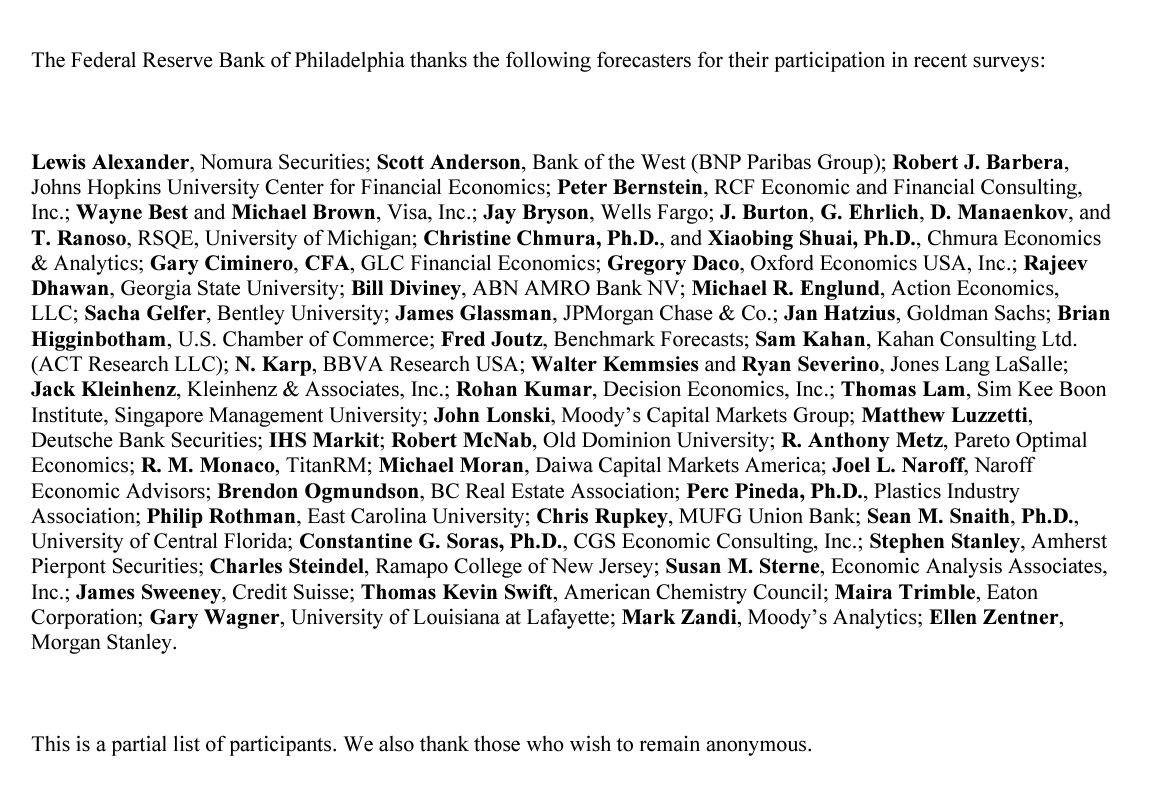
\includegraphics[width=\textwidth]{figures/forecaster_thanks.png}
    \caption{\textbf{Example of forecaster acknowledgments}
    \vspace{5pt}\\
    {\footnotesize The figure shows an example of acknowledgments to forecasters who contributed to recent Federal Reserve Bank of Philadelphia surveys.}
    \vspace{5pt}
    }
    \label{fig:forecaster_thanks}
\end{figure}
\clearpage

%%%%%%%%%%%%%%%%%%%%%%%%%%%

\begin{figure}[h!]
    \centering
    \begin{minipage}{0.48\textwidth}
        \subfloat[Gender]{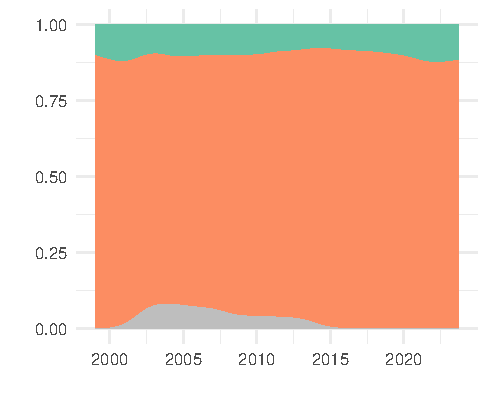
\includegraphics{figures/gender2_over_time.pdf}}\\
        \vskip-1cm
        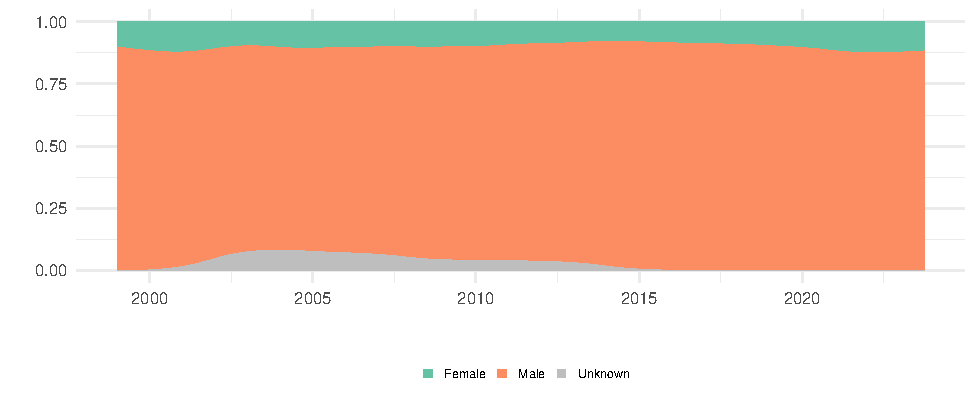
\includegraphics[trim={4.3cm 0 2cm 5.5cm},clip]
        {figures/gender2_over_time_lgd.pdf} 
    \end{minipage}
    \hfill
    \begin{minipage}{0.48\textwidth}
        \subfloat[Graduation Year]{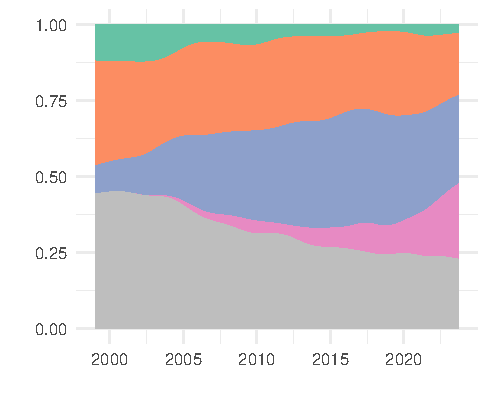
\includegraphics{figures/cohort_over_time.pdf}}\\
        \vskip-1cm
        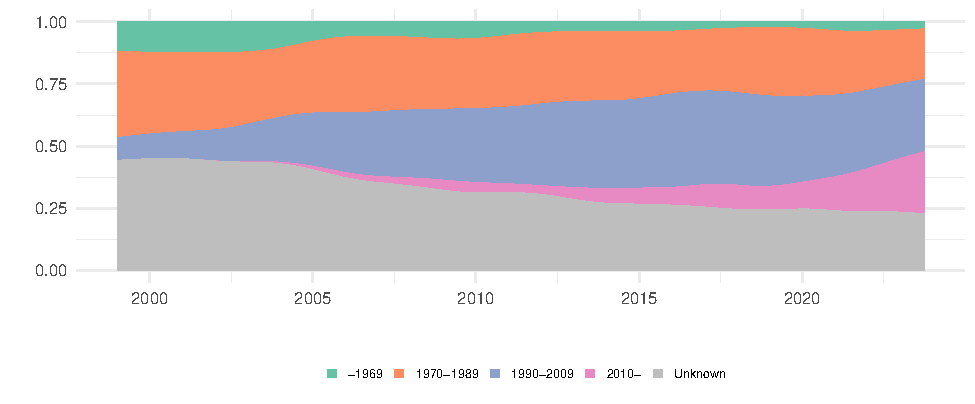
\includegraphics[trim={4.3cm 0 2cm 5.5cm},clip]{figures/cohort_over_time_lgd.pdf} 
    \end{minipage}
    \bigskip
    
    \begin{minipage}{0.48\textwidth}
        \subfloat[Continent of Origin]{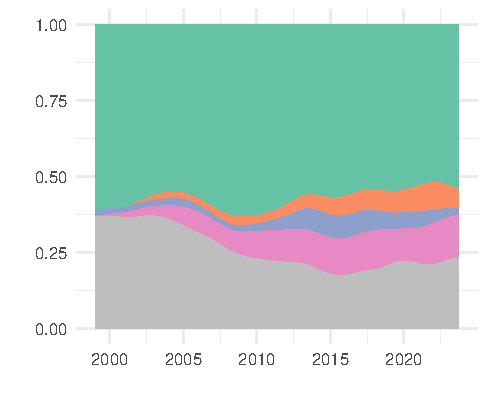
\includegraphics{figures/continent_origin_over_time.pdf}}\\
        \vskip-1cm
        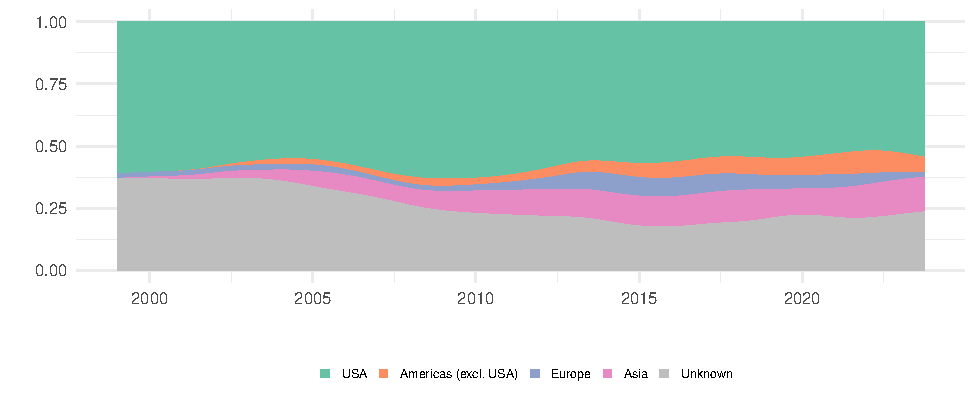
\includegraphics[trim={4.3cm 0 2cm 5.5cm},clip]{figures/continent_origin_over_time_lgd.pdf} 
    \end{minipage}
    \hfill
    \begin{minipage}{0.48\textwidth}
        \subfloat[Public Appearance]{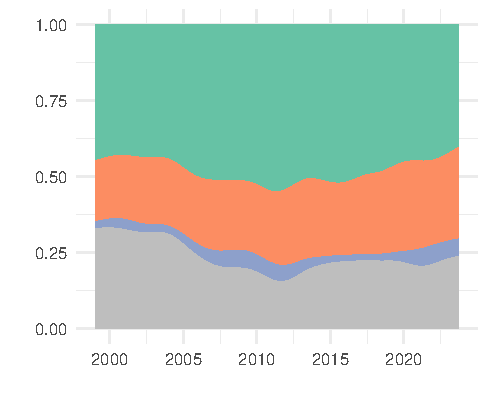
\includegraphics{figures/social_media_status2_over_time.pdf}}\\
        \vskip-1cm
        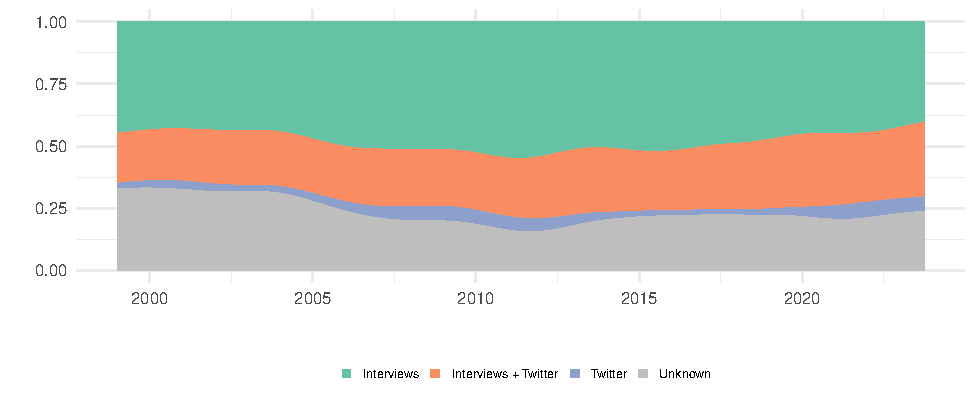
\includegraphics[trim={4.3cm 0 2cm 5.5cm},clip]{figures/social_media_status2_over_time_lgd.pdf} 
    \end{minipage}
    \\\bigskip
    
    \emph{(Figure continues on next page)}
    
    \caption{\textbf{Characteristics of the SPF panel over time}
    \vspace{5pt}\\
    {\footnotesize The figures show the characteristics of the AI SPF panel over time: (a) gender, (b) graduation year, (c) continent of origin, (d) public appearance; on next page: (e) education level, (f) education field, (g) affiliation type, and (h) job title.}
    \vspace{5pt}
    }
    \label{fig:SPF_characteristics_over_time}
\end{figure}
\clearpage

%%%%%%%%%%%%%%%%%%%%%%%%%%%

\begin{figure}[h!]\ContinuedFloat
    \centering
    \begin{minipage}{0.48\textwidth}
        \subfloat[Education level]{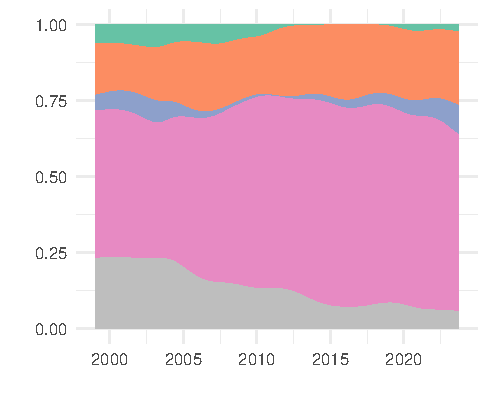
\includegraphics{figures/education_level_over_time.pdf}}\\
        \vskip-1cm
        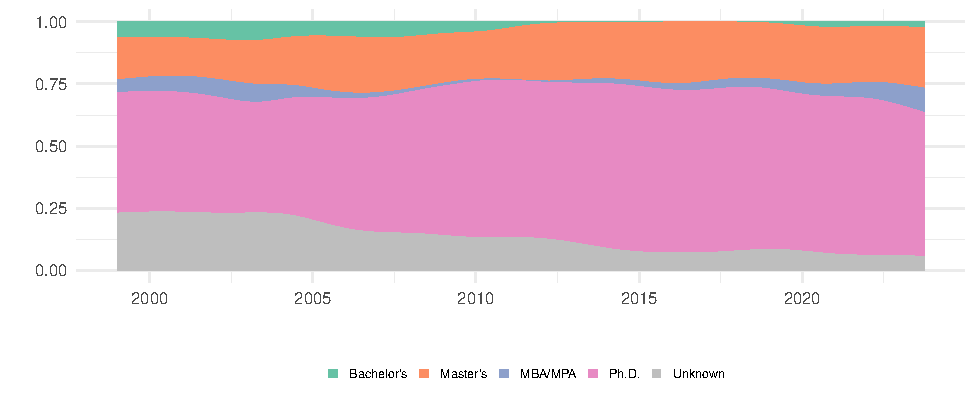
\includegraphics[trim={4.3cm 0 2cm 5.5cm},clip]{figures/education_level_over_time_lgd.pdf} 
    \end{minipage}
    \hfill
    \begin{minipage}{0.48\textwidth}
        \subfloat[Education field]{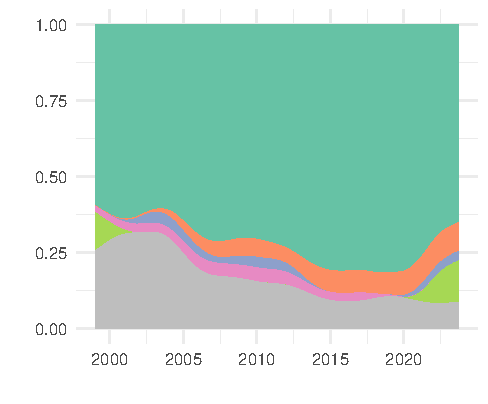
\includegraphics{figures/education_field_over_time.pdf}}\\
        \vskip-1cm
        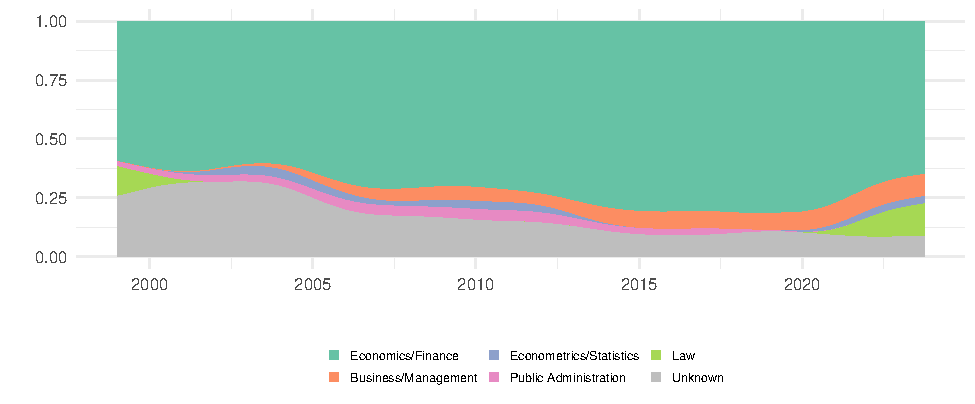
\includegraphics[trim={4.3cm 0 2cm 5.5cm},clip]{figures/education_field_over_time_lgd.pdf} 
    \end{minipage}
    \bigskip
    
    \begin{minipage}{0.48\textwidth}
        \subfloat[Affiliation type]{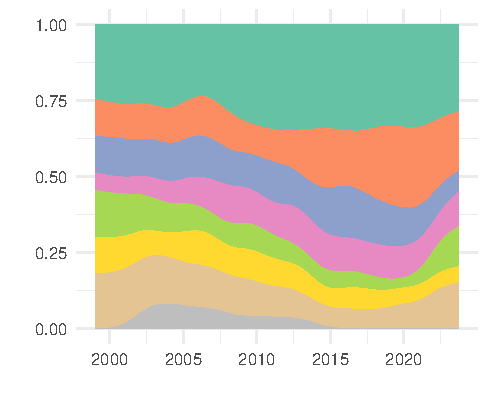
\includegraphics{figures/affiliation_type2_over_time.pdf}}\\
        \vskip-1cm
        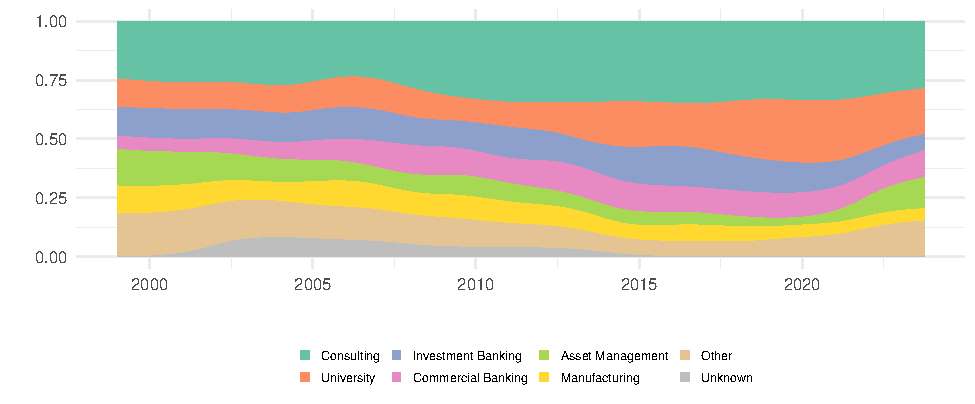
\includegraphics[trim={4.3cm 0 2cm 5.5cm},clip]{figures/affiliation_type2_over_time_lgd.pdf} 
    \end{minipage}
    \hfill
    \begin{minipage}{0.48\textwidth}
        \subfloat[Job title]{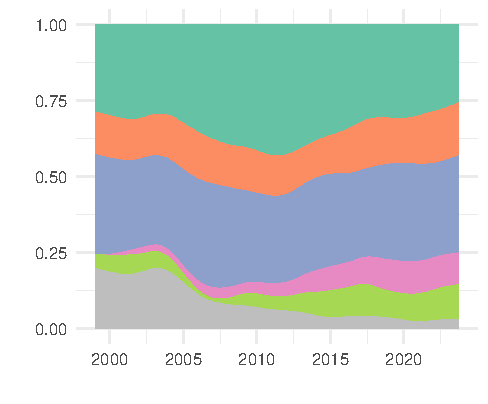
\includegraphics{figures/title2_over_time.pdf}}\\
        \vskip-1cm
        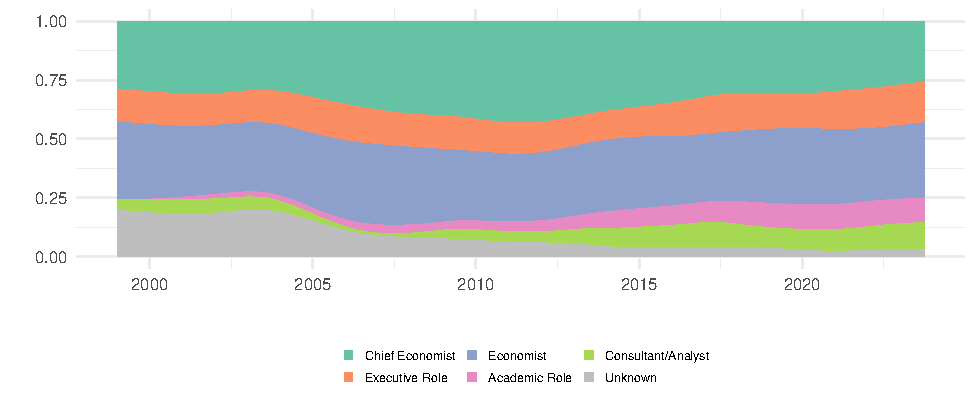
\includegraphics[trim={4.3cm 0 2cm 5.5cm},clip]{figures/title2_over_time_lgd.pdf} 
    \end{minipage}
    
    \caption{\textbf{Characteristics of the AI SPF panel over time} \textit{(continued)}}
    \label{fig:SPF_AI_characteristics}
\end{figure}
\clearpage

%%%%%%%%%%%%%%%%%%%%%%%%%%%

\begin{figure}[htpb!]
    \centering
    \subfloat[CPI inflation rate, one quarter ahead]{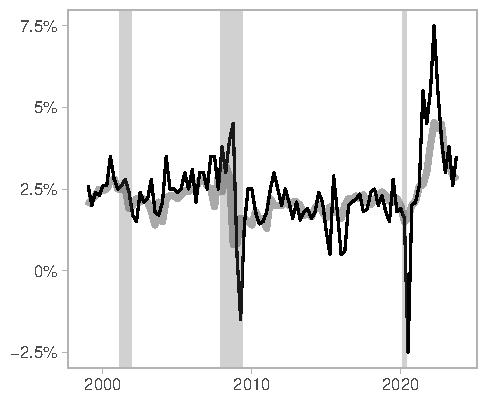
\includegraphics{figures/ts_median_CPI_1.pdf}}
    \subfloat[CPI inflation rate, four quarters ahead]{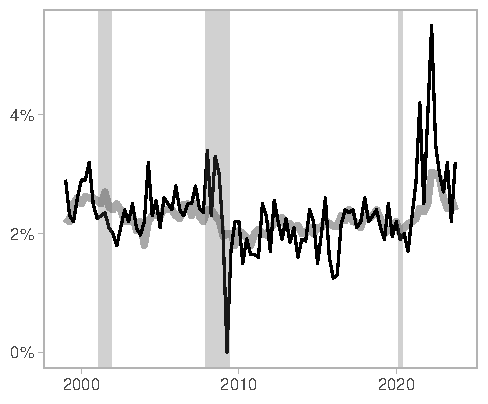
\includegraphics{figures/ts_median_CPI_4.pdf}}\\
    \subfloat[3-month Treasury bill rate, one quarter ahead]{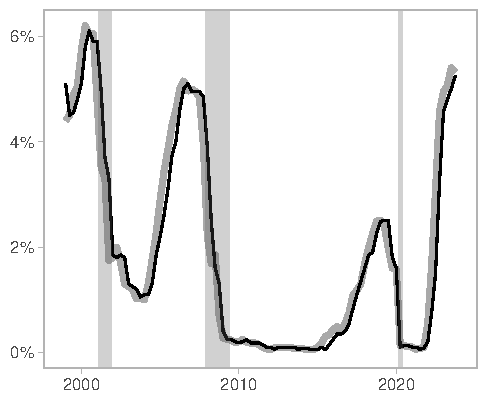
\includegraphics{figures/ts_median_TBILL_1.pdf}}
    \subfloat[3-month Treasury bill rate, four quarters ahead]{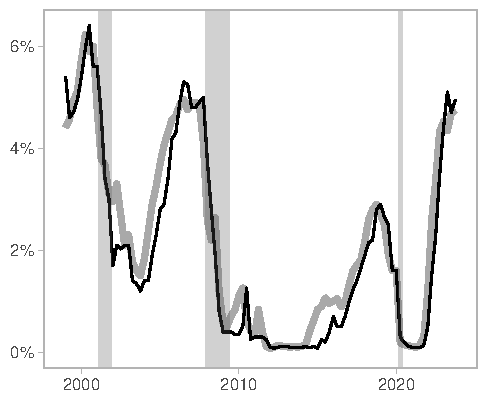
\includegraphics{figures/ts_median_TBILL_4.pdf}}\\
    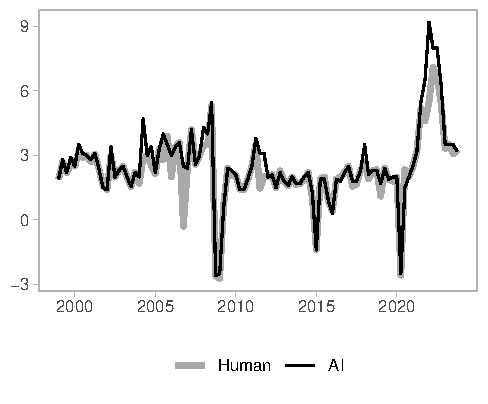
\includegraphics[trim={0 0 0 170pt},clip]{figures/human_ai_lgd.pdf}
    \\
    \emph{(Figure continues on next page)}
    \caption{\textbf{SPF and AI-generated median forecasts}
    \vspace{5pt}\\
    {\footnotesize The figure shows the one- and four-quarter ahead median human and AI-generated SPF forecasts for the (a)-(b) CPI inflation rate, (c)-(d) 3-month Treasury bill rate, (e)-(f) unemployment rate, and (g)-(h) real GDP index. Shaded areas show NBER recession quarters.}
    \vspace{5pt}
    }
    \label{fig:median_forecasts}
\end{figure}
\clearpage
\begin{figure}[h!]\ContinuedFloat
    \centering
    \subfloat[Unemployment rate, one quarter ahead]{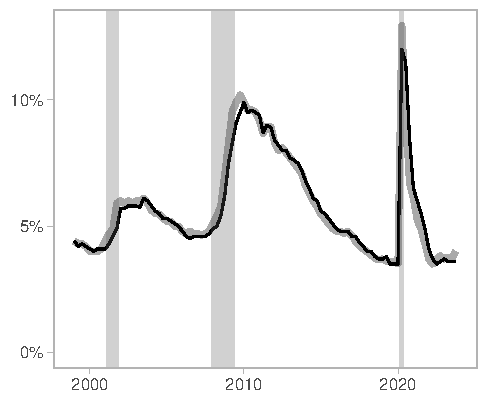
\includegraphics{figures/ts_median_UNEMP_1.pdf}}
    \subfloat[Unemployment rate, four quarters ahead]{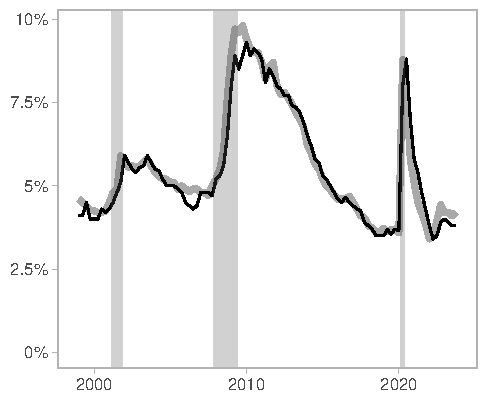
\includegraphics{figures/ts_median_UNEMP_4.pdf}}\\
    \subfloat[Real GDP index, one quarter ahead]{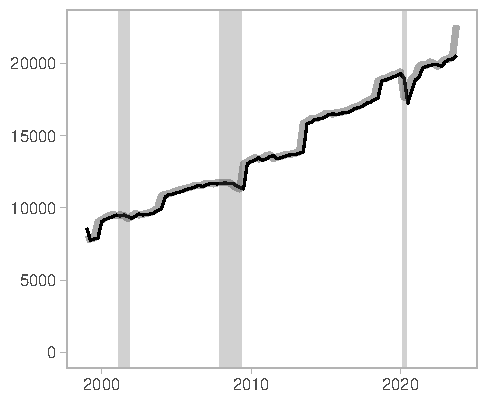
\includegraphics{figures/ts_median_RGDP_1.pdf}}
    \subfloat[Real GDP index, four quarters ahead]{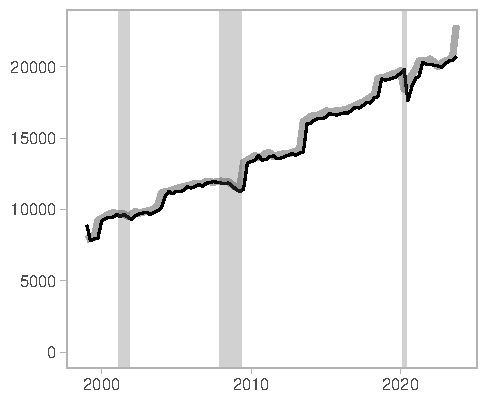
\includegraphics{figures/ts_median_RGDP_4.pdf}}\\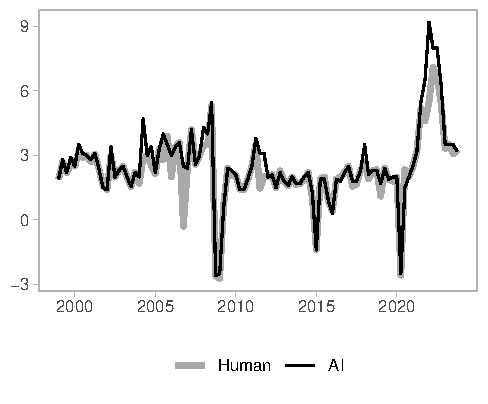
\includegraphics[trim={0 0 0 170pt},clip]{figures/human_ai_lgd.pdf}
    \caption{\textbf{SPF and AI-generated median forecasts} \emph{(continued)}
    \vspace{5pt}
    }
    \label{fig:median_forecasts}
\end{figure}
\clearpage

%%%%%%%%%%%%%%%%%%%%%%%%%%%

\begin{figure}[t]
  \centering
  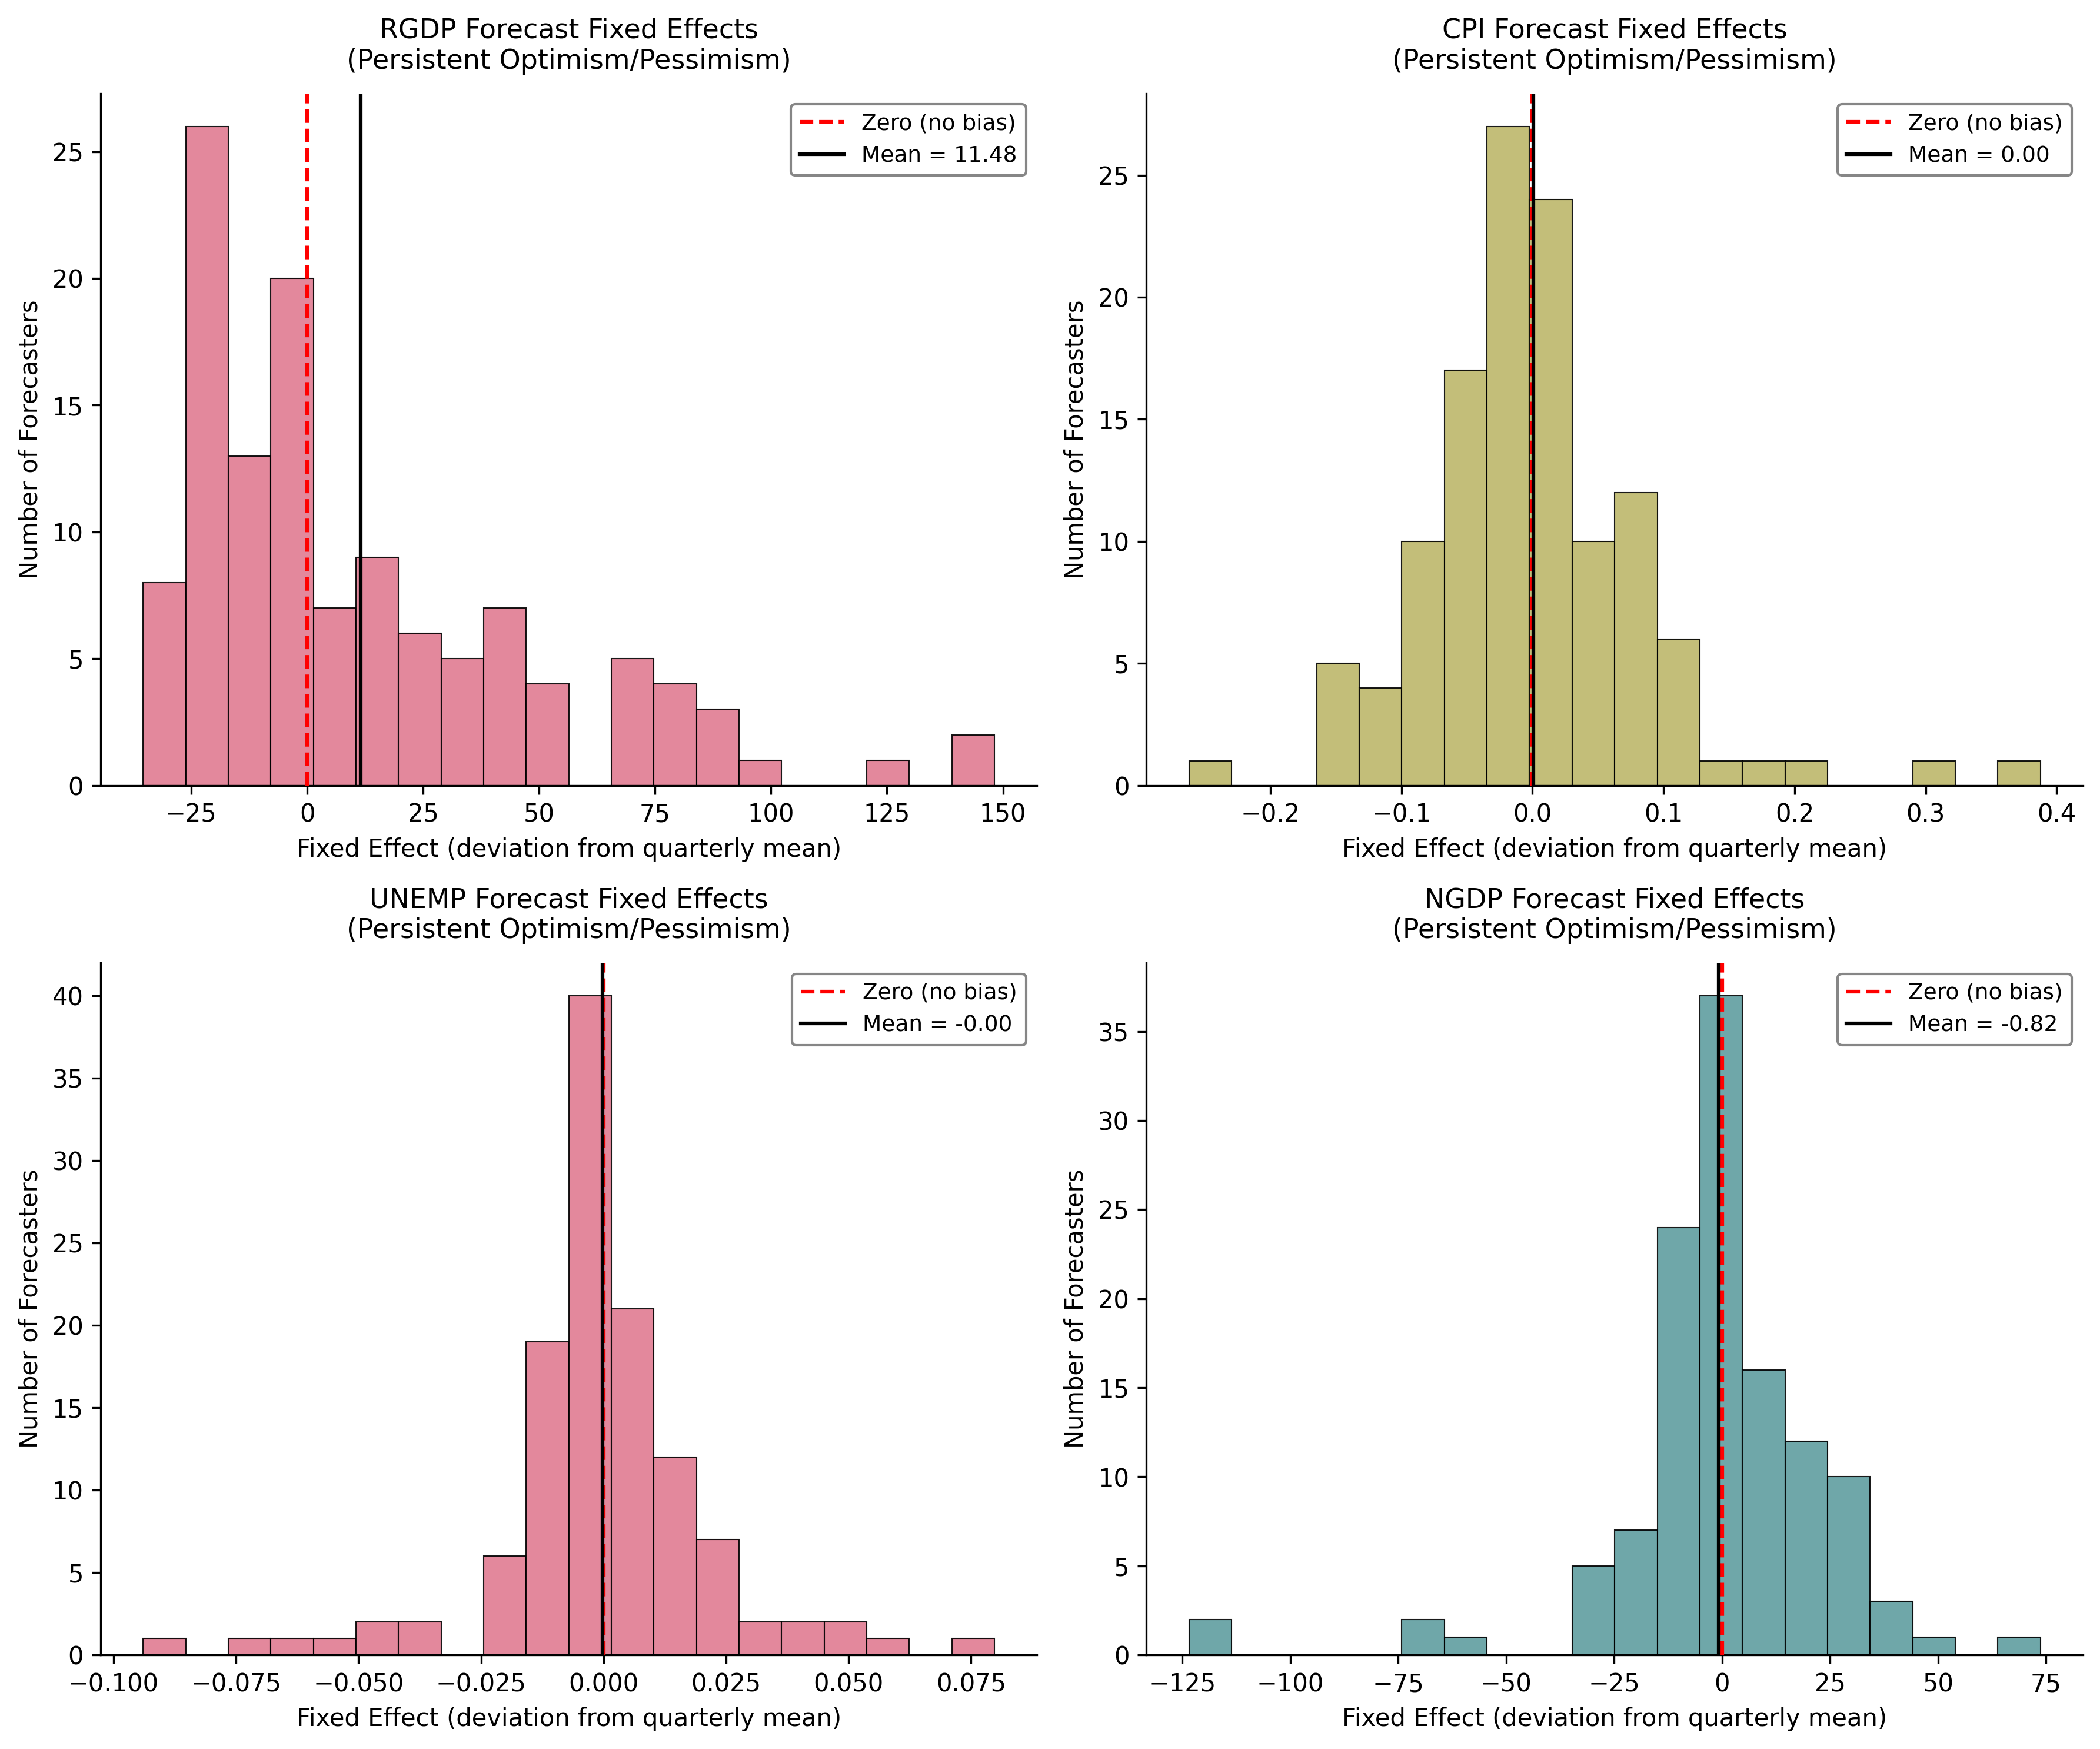
\includegraphics[width=\textwidth]{figures/figure6_fixed_effects_updated.png}
  \caption{Distribution of Forecaster Fixed Effects}
  \label{fig:fixed_effects}
  \vspace{5pt}
  \begin{minipage}{\textwidth}
    \raggedright
    \footnotesize \textit{Notes:} The figure shows the distribution of forecaster-specific fixed effects for four macroeconomic variables. Fixed effects are calculated as the average deviation of each forecaster's prediction from the quarterly cross-sectional mean. Each panel displays a histogram of fixed effects across 194 forecasters, with vertical lines indicating zero (red dashed) and the sample mean (black solid). RGDP and NGDP are measured in billions of 2012 dollars; CPI and UNEMP are measured in percentage points. Forecasters are restricted to those with at least 10 observations across the sample period (1999--2023).
  \end{minipage}
  \vspace{5pt}
\end{figure}

%%%%%%%%%%%%%%%%%%%%%%%%%%%

\begin{figure}[h!]
    \centering
    \subfloat[CPI inflation rate, one quarter ahead]{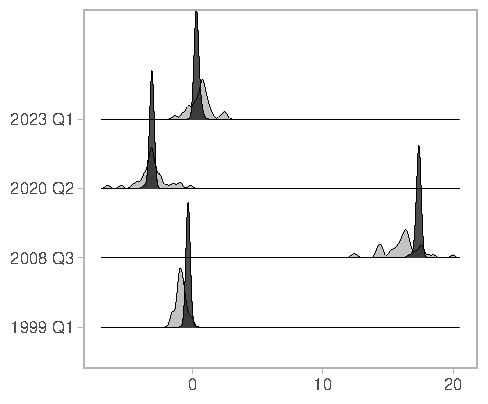
\includegraphics{figures/density_CPI_1.pdf}}
    \subfloat[CPI inflation rate, four quarters ahead]{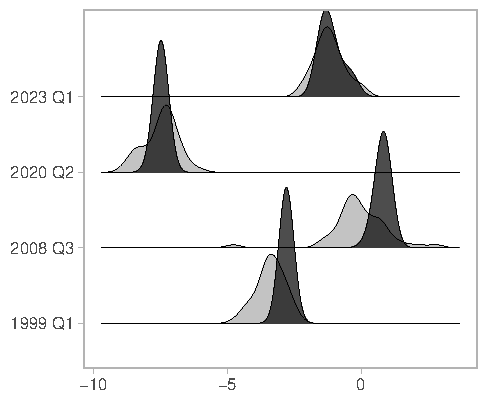
\includegraphics{figures/density_CPI_4.pdf}}\\
    \subfloat[3-month Treasury bill rate, one quarter ahead]{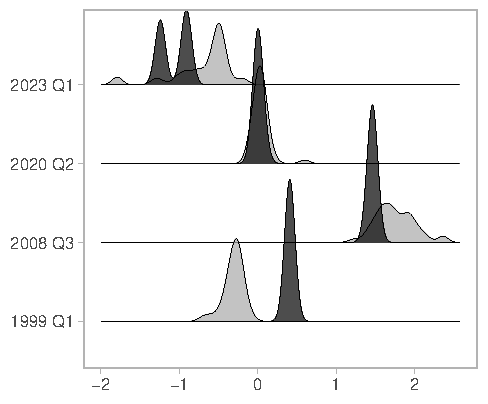
\includegraphics{figures/density_TBILL_1.pdf}}
    \subfloat[3-month Treasury bill rate, four quarters ahead]{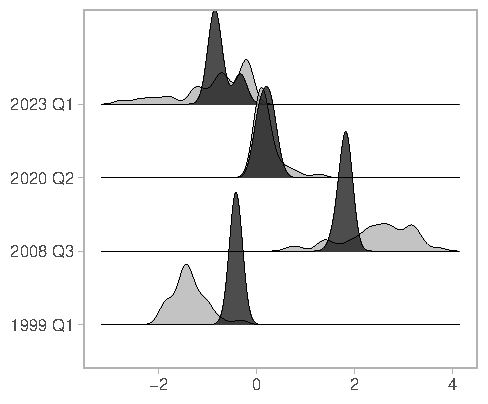
\includegraphics{figures/density_TBILL_4.pdf}}\\
    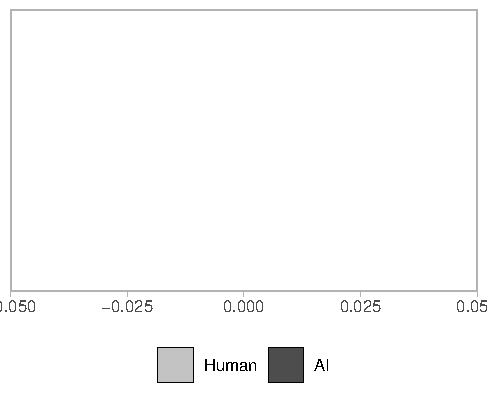
\includegraphics[trim={0 0 0 160pt},clip]{figures/density_lgd.pdf}
    \\
    \emph{(Figure continues on next page)}
    \caption{\textbf{Densities of human and AI-generated SPF individual forecast errors}
    \vspace{5pt}\\
    {\footnotesize The figure shows densities centered around realized variables of human and AI-generated SPF forecasts across individual forecasters for four different quarters. The densities are shown for the following variables and forecasting horizons: (a) CPI inflation rate one quarter ahead, (b) CPI inflation rate four quarters ahead, (c) 3-month Treasury bill rate one quarter ahead, (d) 3-month Treasury bill rate four quarters ahead, (e) unemployment rate one quarter ahead, (f) unemployment rate four quarters ahead, (g) real GDP index one quarter ahead, and (h) real GDP index four quarters ahead.}
    \vspace{5pt}
    }
    \label{fig:density_AI_SPF}
\end{figure}
\clearpage
\begin{figure}[h!]\ContinuedFloat
    \centering
    \subfloat[Unemployment rate, one quarter ahead]{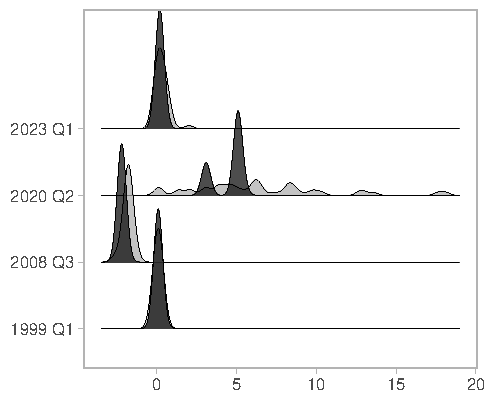
\includegraphics{figures/density_UNEMP_1.pdf}}
    \subfloat[Unemployment rate, four quarters ahead]{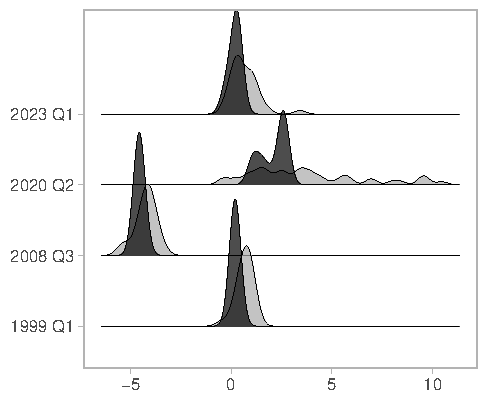
\includegraphics{figures/density_UNEMP_4.pdf}}\\
    \subfloat[Real GDP index, one quarter ahead]{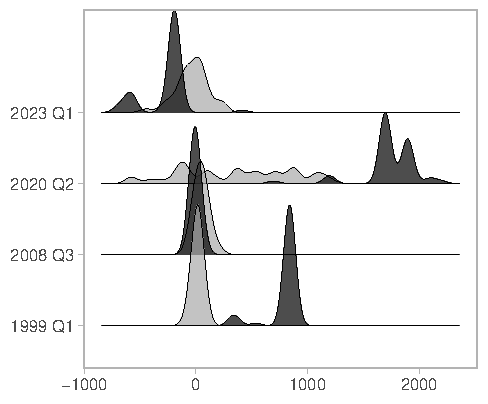
\includegraphics{figures/density_RGDP_1.pdf}}
    \subfloat[Real GDP index, four quarters ahead]{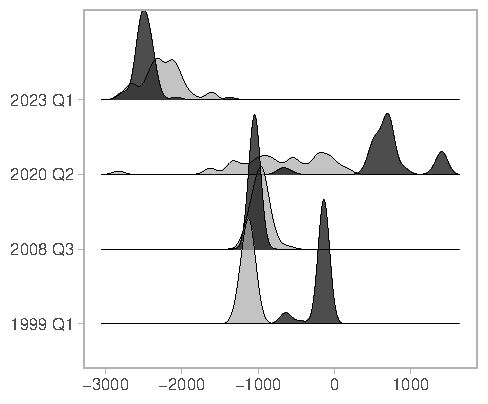
\includegraphics{figures/density_RGDP_4.pdf}}\\
    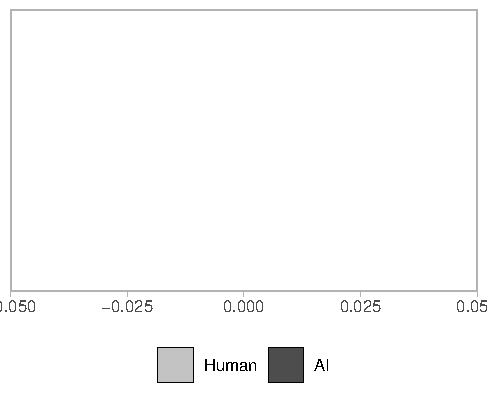
\includegraphics[trim={0 0 0 160pt},clip]{figures/density_lgd.pdf}
    \caption{\textbf{Densities of human and AI-generated SPF individual forecast errors} \emph{(continued)}
    \vspace{5pt}
    }
\end{figure}

\begin{comment}
\begin{figure}
    \centering
    \caption{\textbf{Coefficients from regressing individual forecast errors on characteristics}
    \vspace{5pt}\\
    \footnotesize{The figure shows coefficients from regressing individual AI-generated forecasts on characteristic dummy variables. All coefficients should be interpreted relative to the baseline where the characteristic is unknown. The coefficients are estimated using the sparse-group LASSO approach from \cite{babii2022machine}. Coefficients shaded in darker blue (red) indicate that the characteristics are associated with improved (worsened) forecast accuracy.} 
    }
    \subfloat[Nowcast]{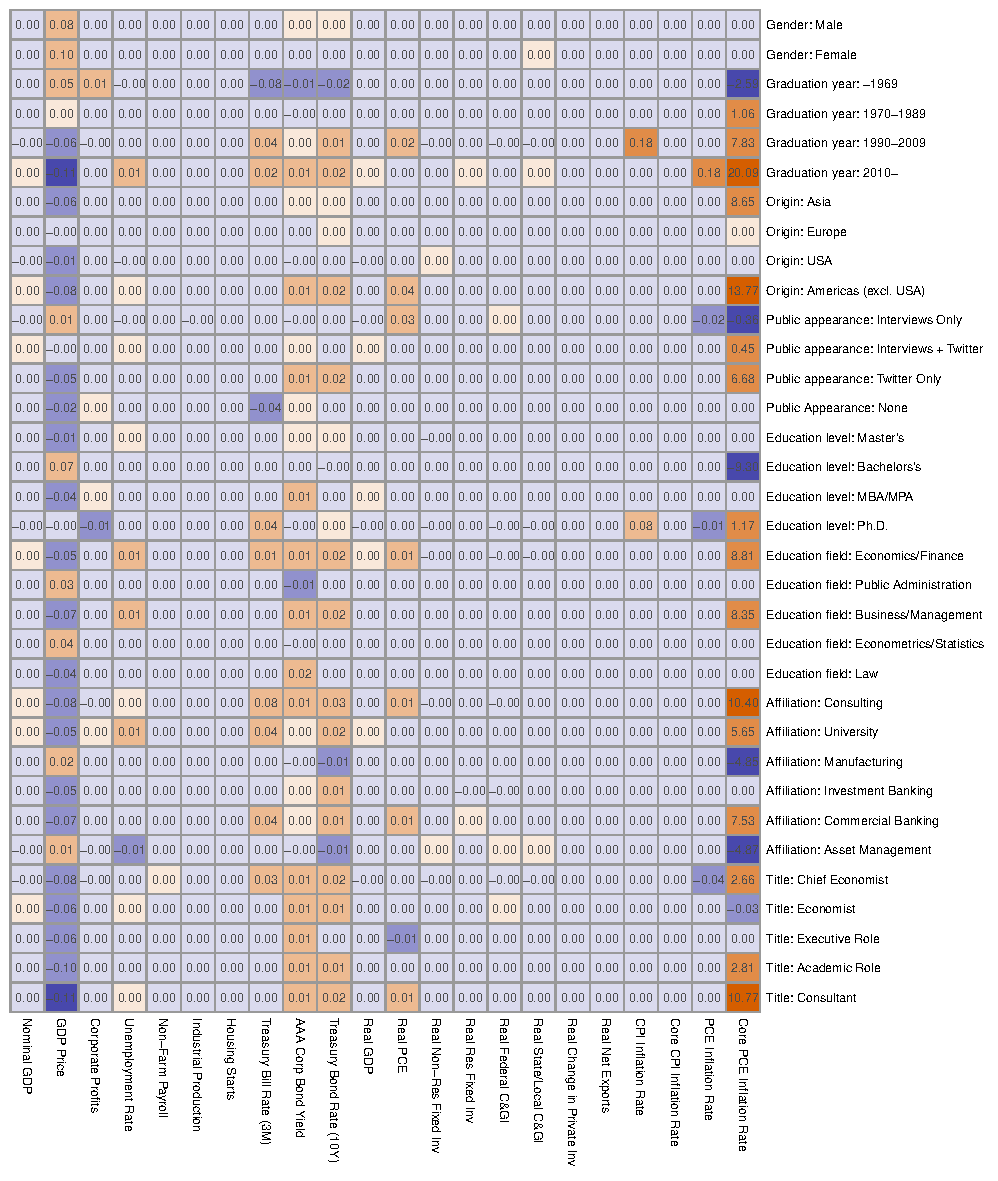
\includegraphics{figures/lasso_characteristics_aic_0.pdf}}
    \\
    \emph{(Figure continues on next page)}
    \label{fig:lasso_characteristics}
\end{figure}
\thispagestyle{empty}
\clearpage

\begin{figure}\ContinuedFloat
    \centering
    \caption{\textbf{Coefficients from regressing individual forecast errors on characteristics} \emph{(continued)}
    }
    \subfloat[Four-quarters ahead forecast]{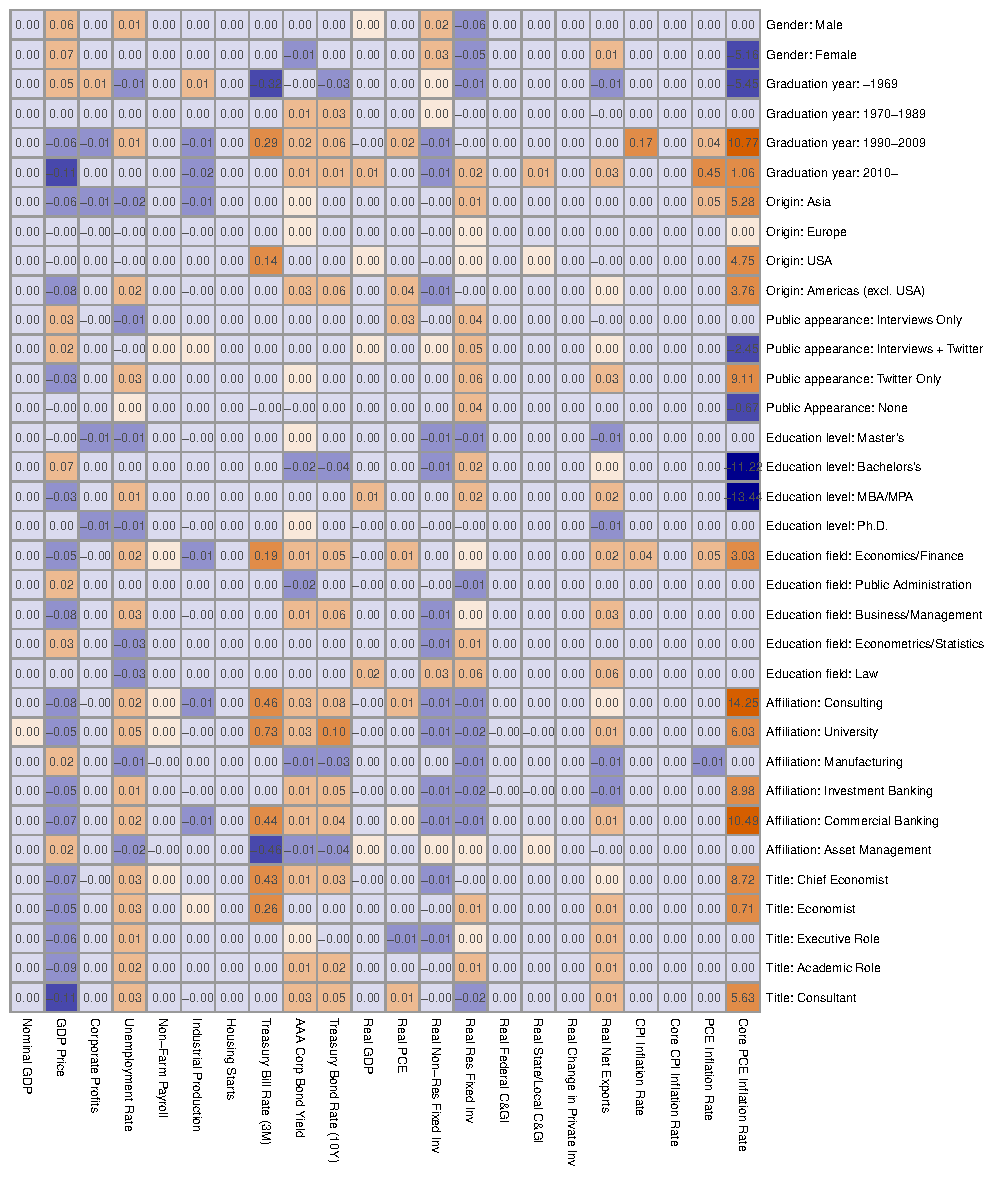
\includegraphics{figures/lasso_characteristics_aic_4.pdf}}
\end{figure}
\clearpage
\end{comment}

\begin{comment}
\begin{figure}[h!]
    \centering
    \subfloat[Nowcast]{\includegraphics{figures/ts_median_UNEMP_0_WSJ.pdf}}\\
    \subfloat[Two quarters ahead]{\includegraphics{figures/ts_median_UNEMP_2_WSJ.pdf}}\\
    \subfloat[Four quarters ahead]{\includegraphics{figures/ts_median_UNEMP_4_WSJ.pdf}}
    \\
    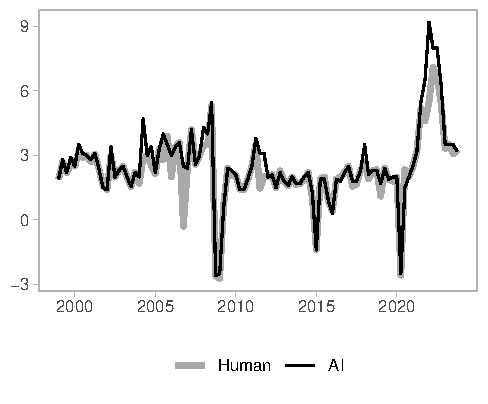
\includegraphics[trim={0 0 0 170pt},clip]{figures/human_ai_lgd.pdf}\\
    \caption{\textbf{WSJ and AI-generated median forecasts}
    \vspace{5pt}\\
    {\footnotesize The figure shows median WSJ forecasts and AI-generated forecasts of the unemployment rate across three forecasting horizons: Nowcast, two quarters ahead, and four quarters ahead. Shaded areas show NBER recession quarters.}
    \vspace{5pt}
    }
    \label{fig:median_forecasts_WSJ}
\end{figure}
\clearpage

\begin{figure}[h!]
    \centering
    \subfloat[Nowcast]{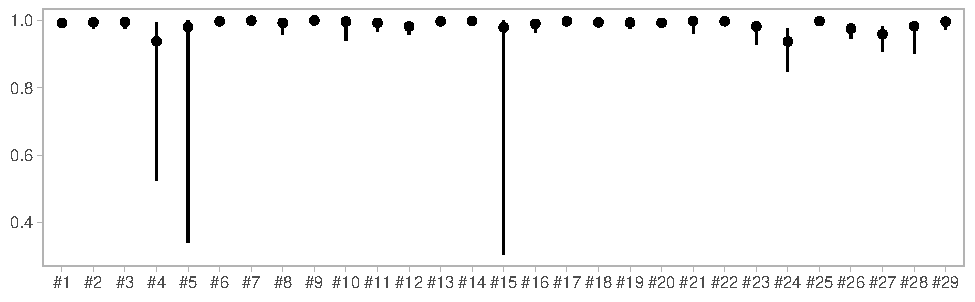
\includegraphics{figures/correlations_0_WSJ.pdf}}\\
    \subfloat[Two quarters ahead]{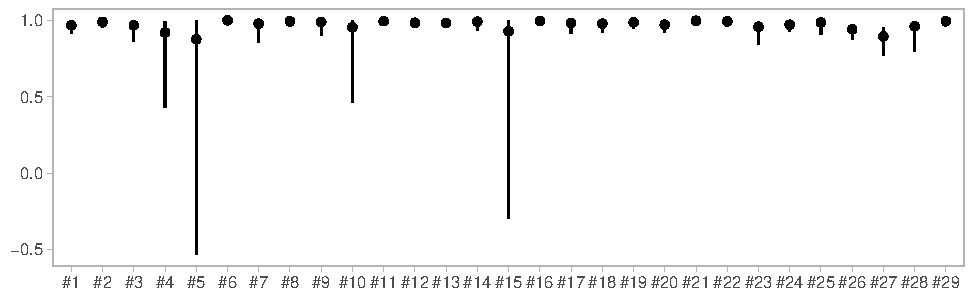
\includegraphics{figures/correlations_2_WSJ.pdf}}\\
    \subfloat[Four quarters ahead]{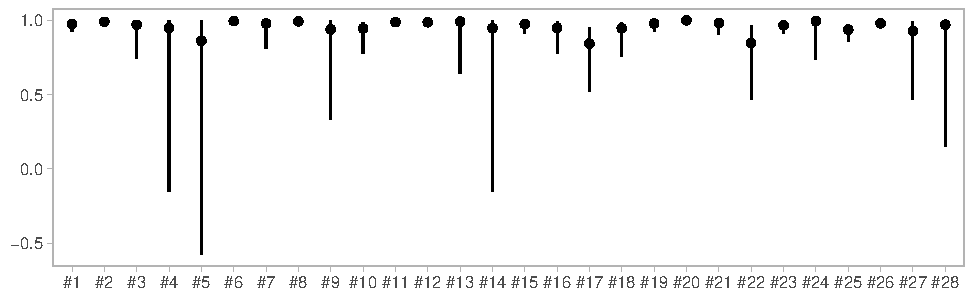
\includegraphics{figures/correlations_4_WSJ.pdf}}
    \\
    \caption{\textbf{Correlations between WSJ and AI-generated forecasts by each individual forecast}
    \vspace{5pt}\\
    {\footnotesize The figure shows the correlation between WSJ forecasts and AI-generated forecasts of the unemployment rate for each individual forecaster (numbered on the primary axis). Results are shown across three forecasting horizons: Nowcast, two quarters ahead, and four quarters ahead. The vertical lines show 95\% confidence intervals.}
    \vspace{5pt}
    }
    \label{fig:correlation_WSJ}
\end{figure}
\clearpage
\end{comment}

\begin{comment}
\begin{figure}[htbp!]
    \centering
    \caption{\textbf{Comparison of average SPF and WSJ forecasts for Unemployment Rate (UR)}}
    \vspace{5pt}\\
    \raggedright
    \footnotesize{\textit{Note:} This figure presents the comparison between the average WSJ and SPF forecasts for the unemployment rate (UR, on y-axis) across three forecast horizons: nowcast (the current quarter, top graph), 2-quarter ahead (middle graph), and 4-quarter ahead (bottom graph).} 
    \vspace{2em}\\
    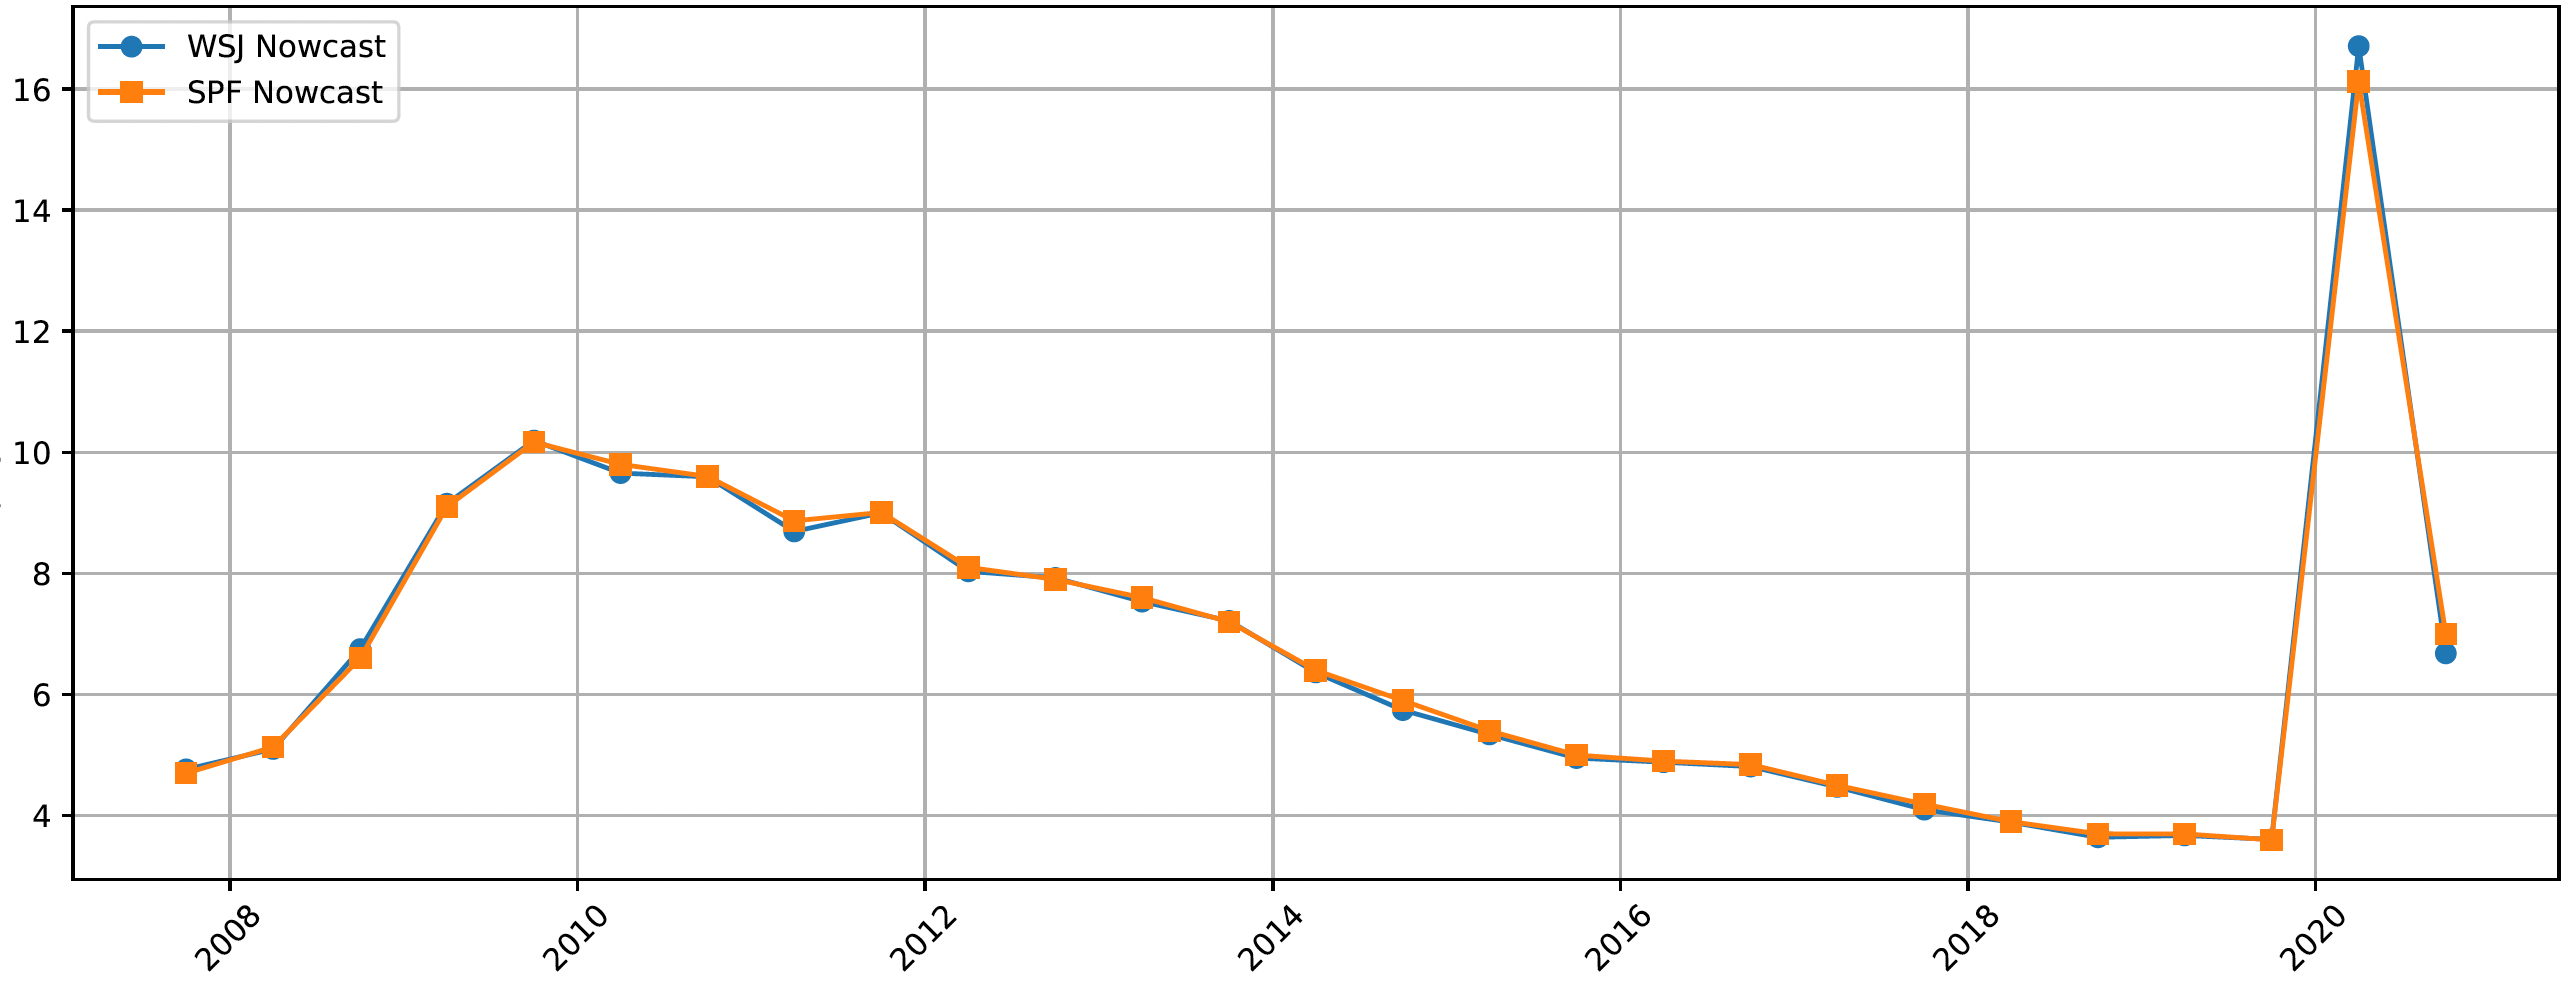
\includegraphics[width=\textwidth]{figures/nowcast_spf_wsj.png} \\[10pt] %
    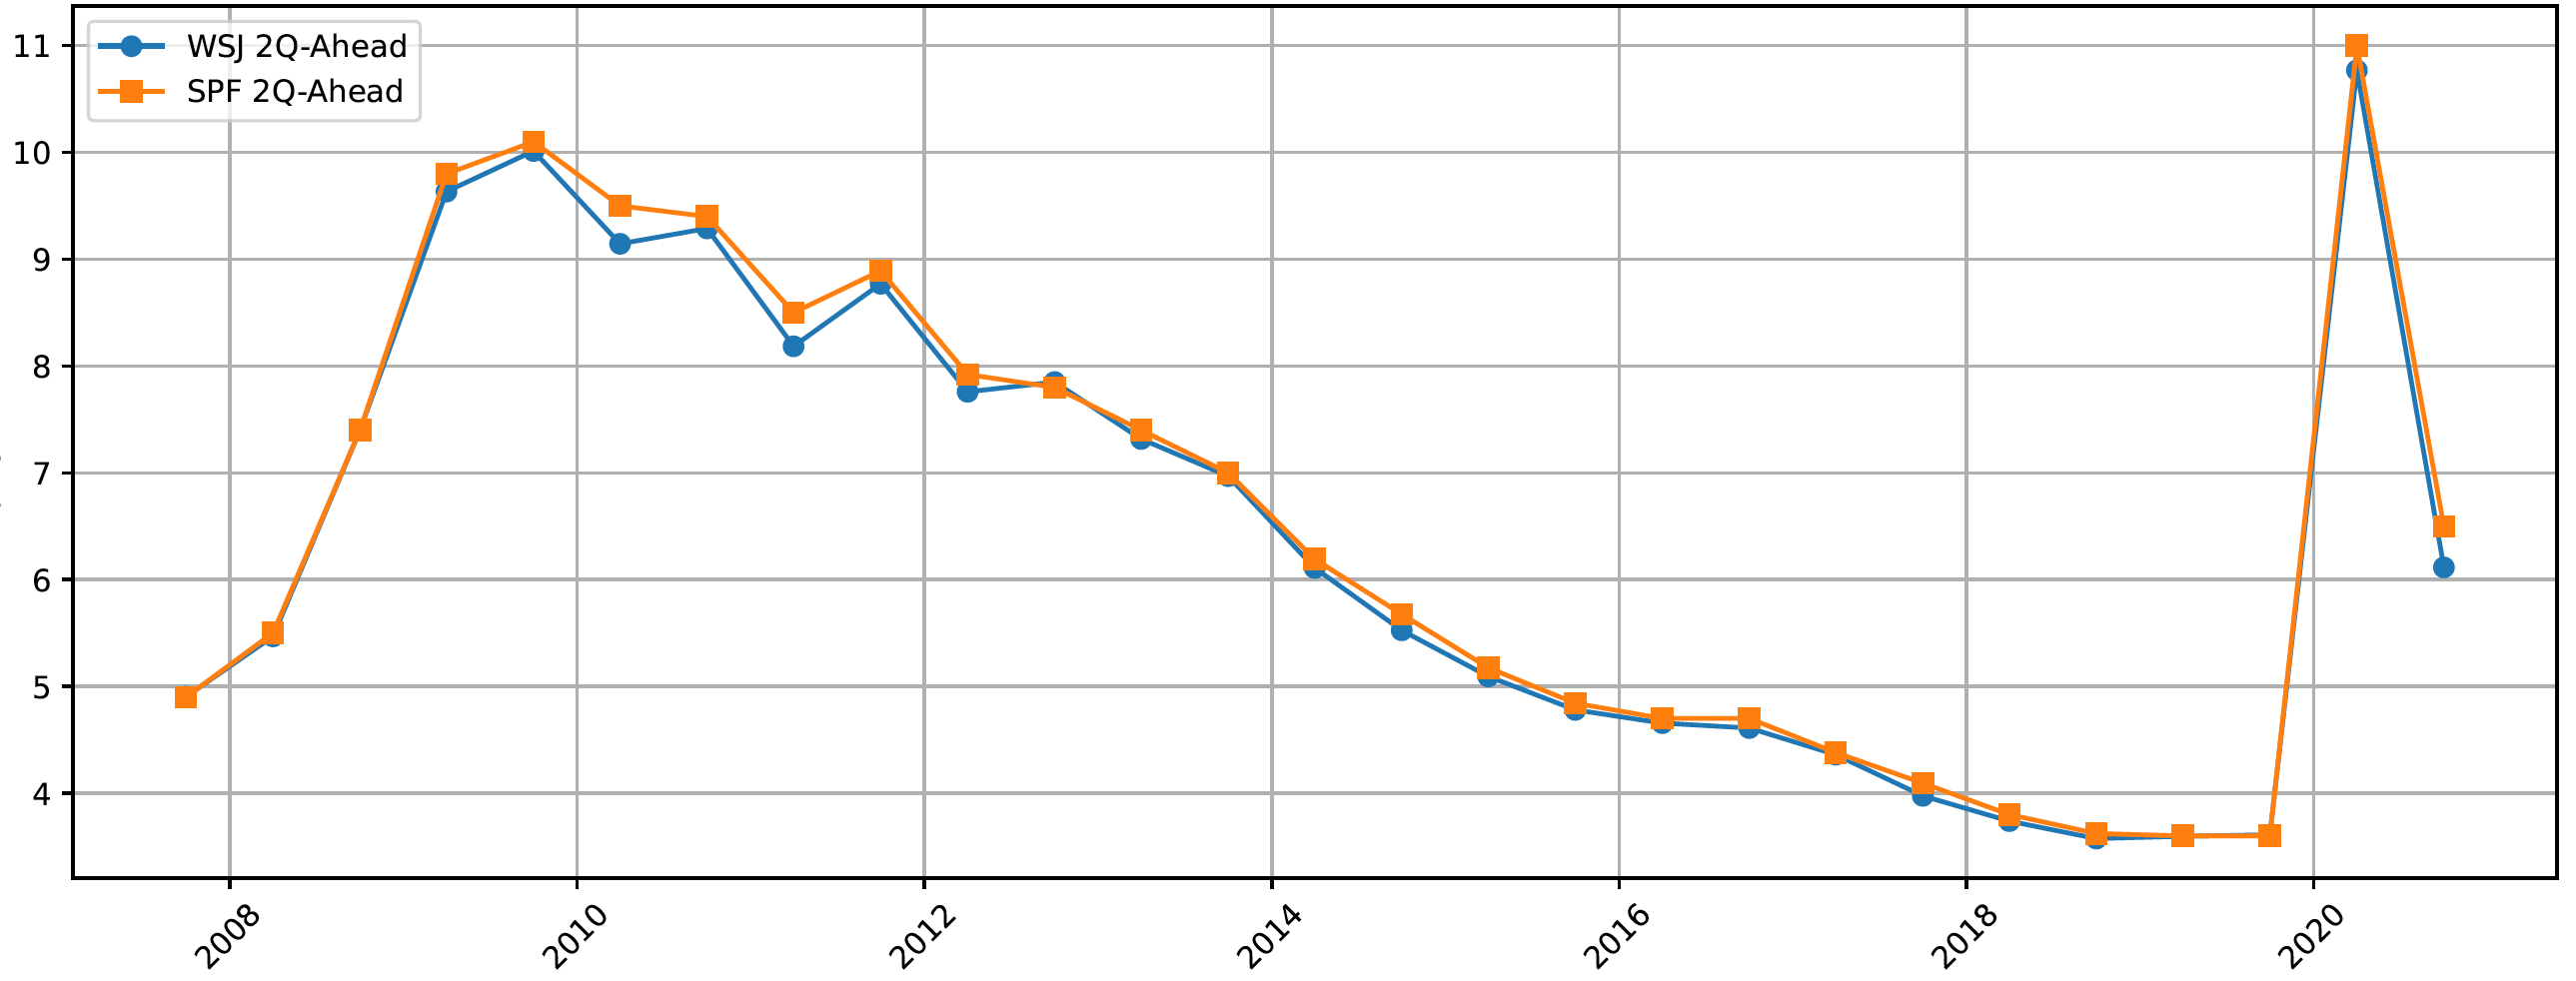
\includegraphics[width=\textwidth]{figures/2q_spf_wsj.png} \\[10pt] 
    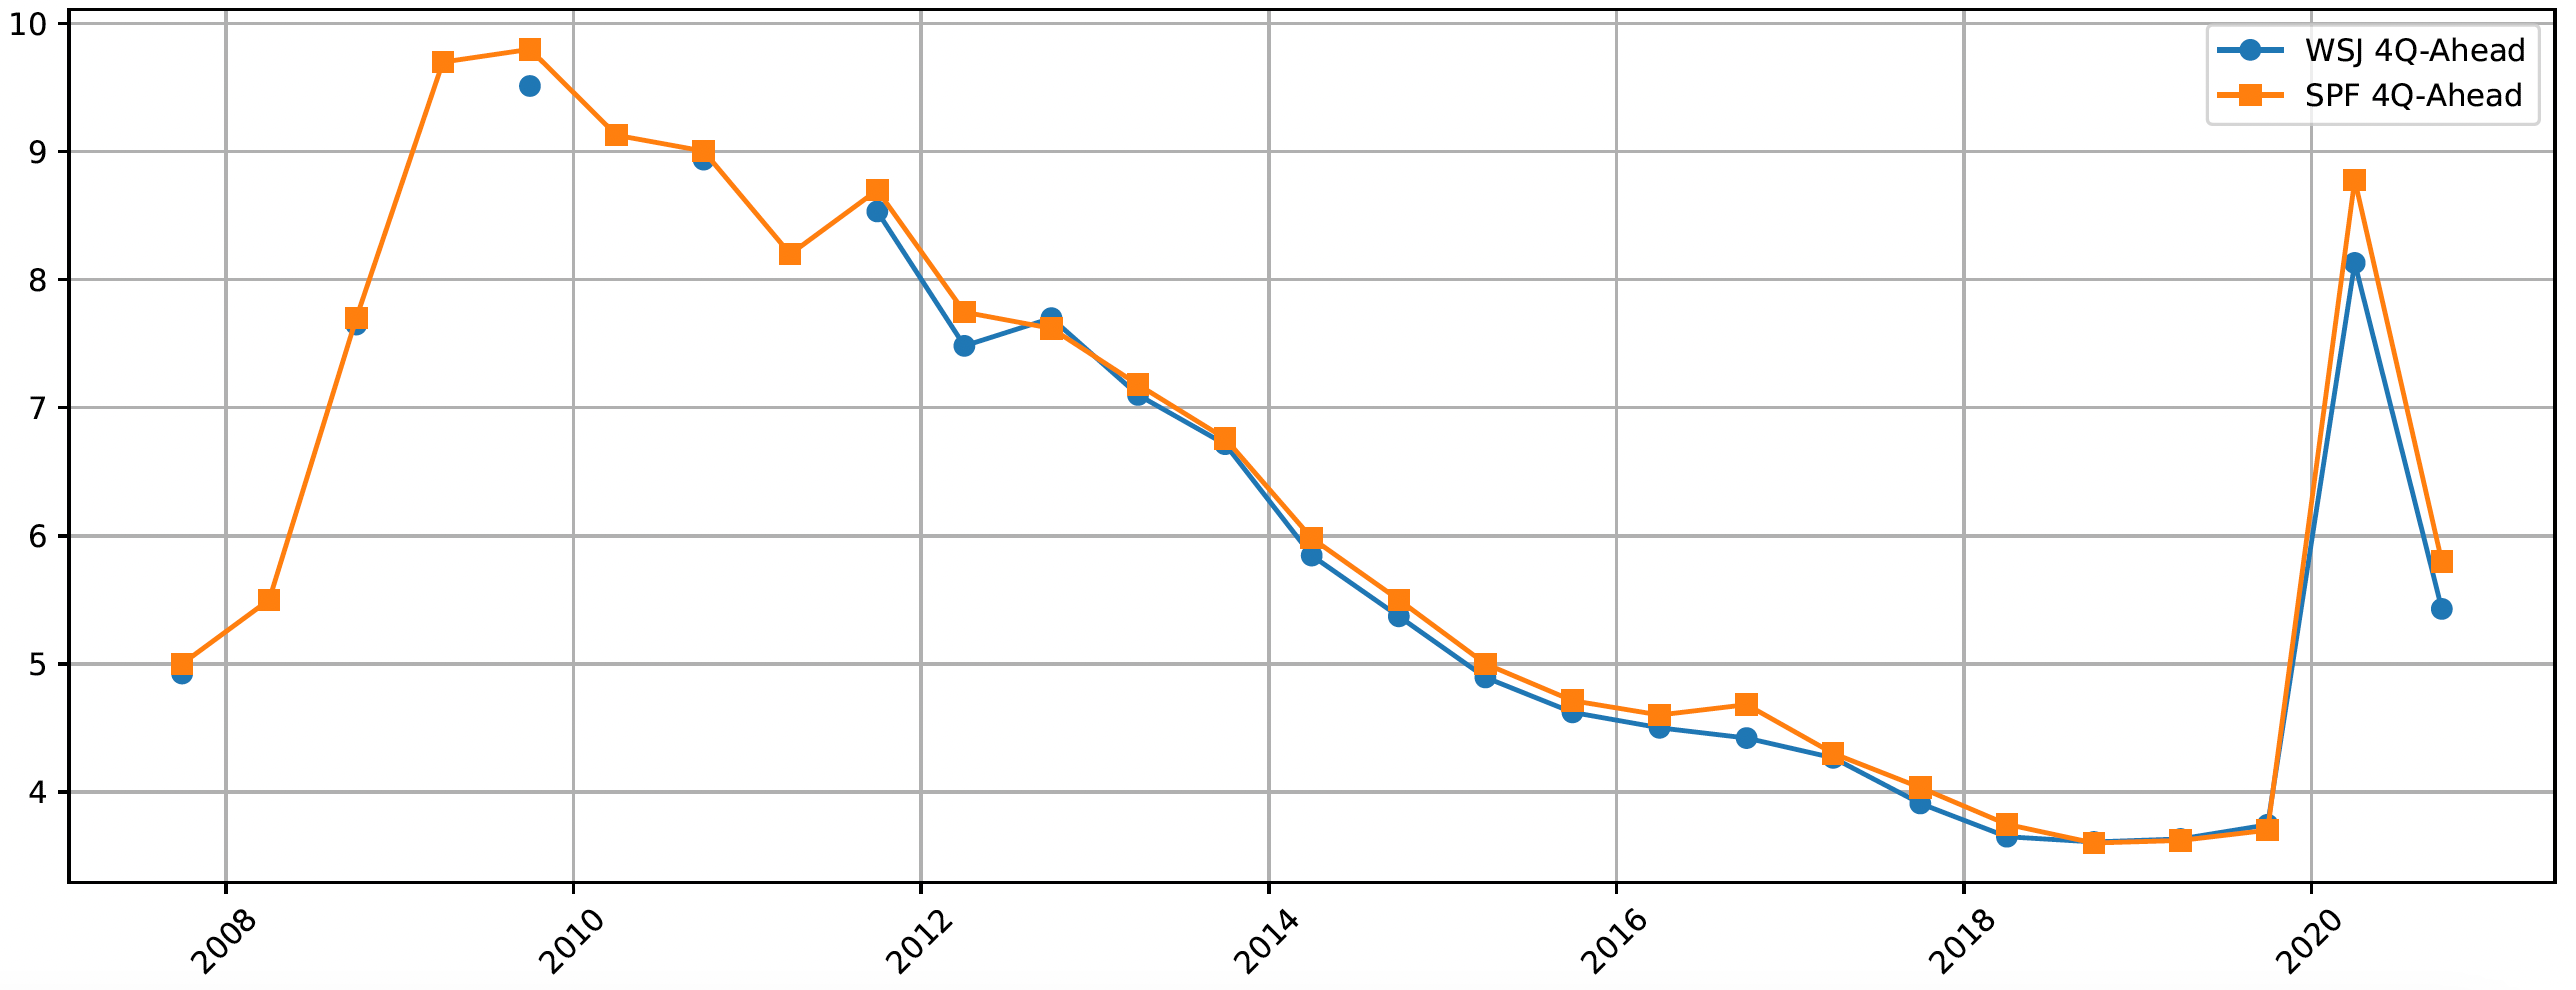
\includegraphics[width=\textwidth]{figures/4q_spf_wsj.png} 
    \label{fig:wsj_spf_comparison}
\end{figure}
\end{comment}

\begin{figure}[htpb!]
    \centering
    \subfloat[CPI inflation rate, one quarter ahead]{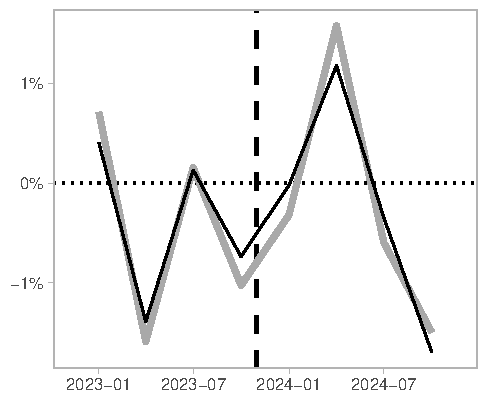
\includegraphics{figures/forecast_error_oos_CPI_1.pdf}}
    \subfloat[3-month Treasury bill rate, one quarter ahead]{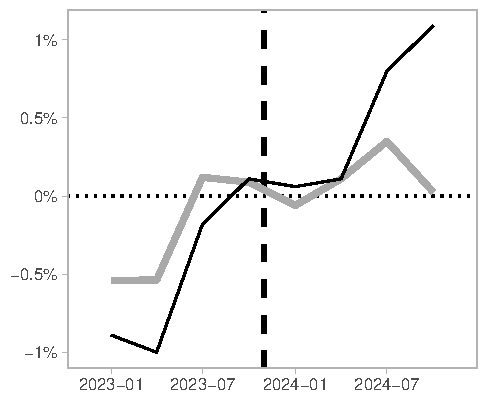
\includegraphics{figures/forecast_error_oos_TBILL_1.pdf}}\\
    \subfloat[Unemployment rate, one quarter ahead]{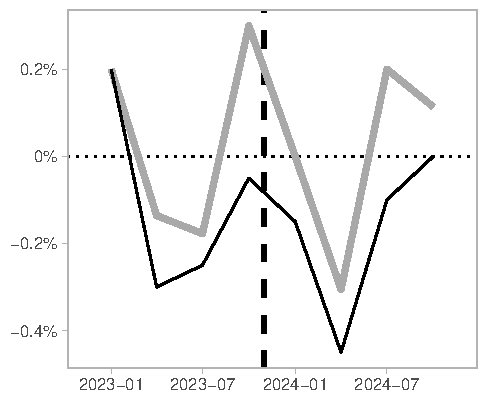
\includegraphics{figures/forecast_error_oos_UNEMP_1.pdf}}
    \subfloat[Real GDP, one quarter ahead]{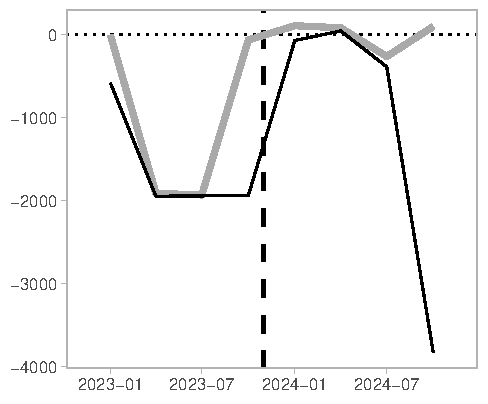
\includegraphics{figures/forecast_error_oos_RGDP_1.pdf}}\\
    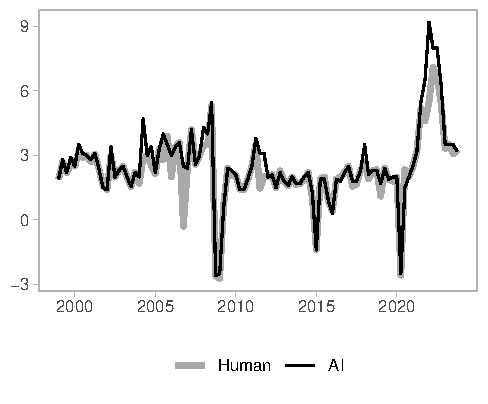
\includegraphics[trim={0 0 0 170pt},clip]{figures/human_ai_lgd.pdf}
    \\
    \caption{\textbf{SPF and AI-generated median forecast errors around the LLM training data cut-off date}
    \vspace{5pt}\\
    {\footnotesize The figure shows the errors of one-quarter human and AI-generated SPF median forecasts for the (a) CPI inflation rate, (b) 3-month Treasury bill rate, (c) unemployment rate, and (d) real GDP index. The dashed line indicates October 2023, the training data cut-off date of the LLM (GPT-4o mini).}
    \vspace{5pt}
    }
    \label{fig:oos_forecast_errors}
\end{figure}

%%%%%%%%%%%%%%%%%%%%%%%%%%%%%%%%%%%%%%%%%%
\begin{comment}
\begin{figure}[t]
  \centering
  \begin{subfigure}{\textwidth}
    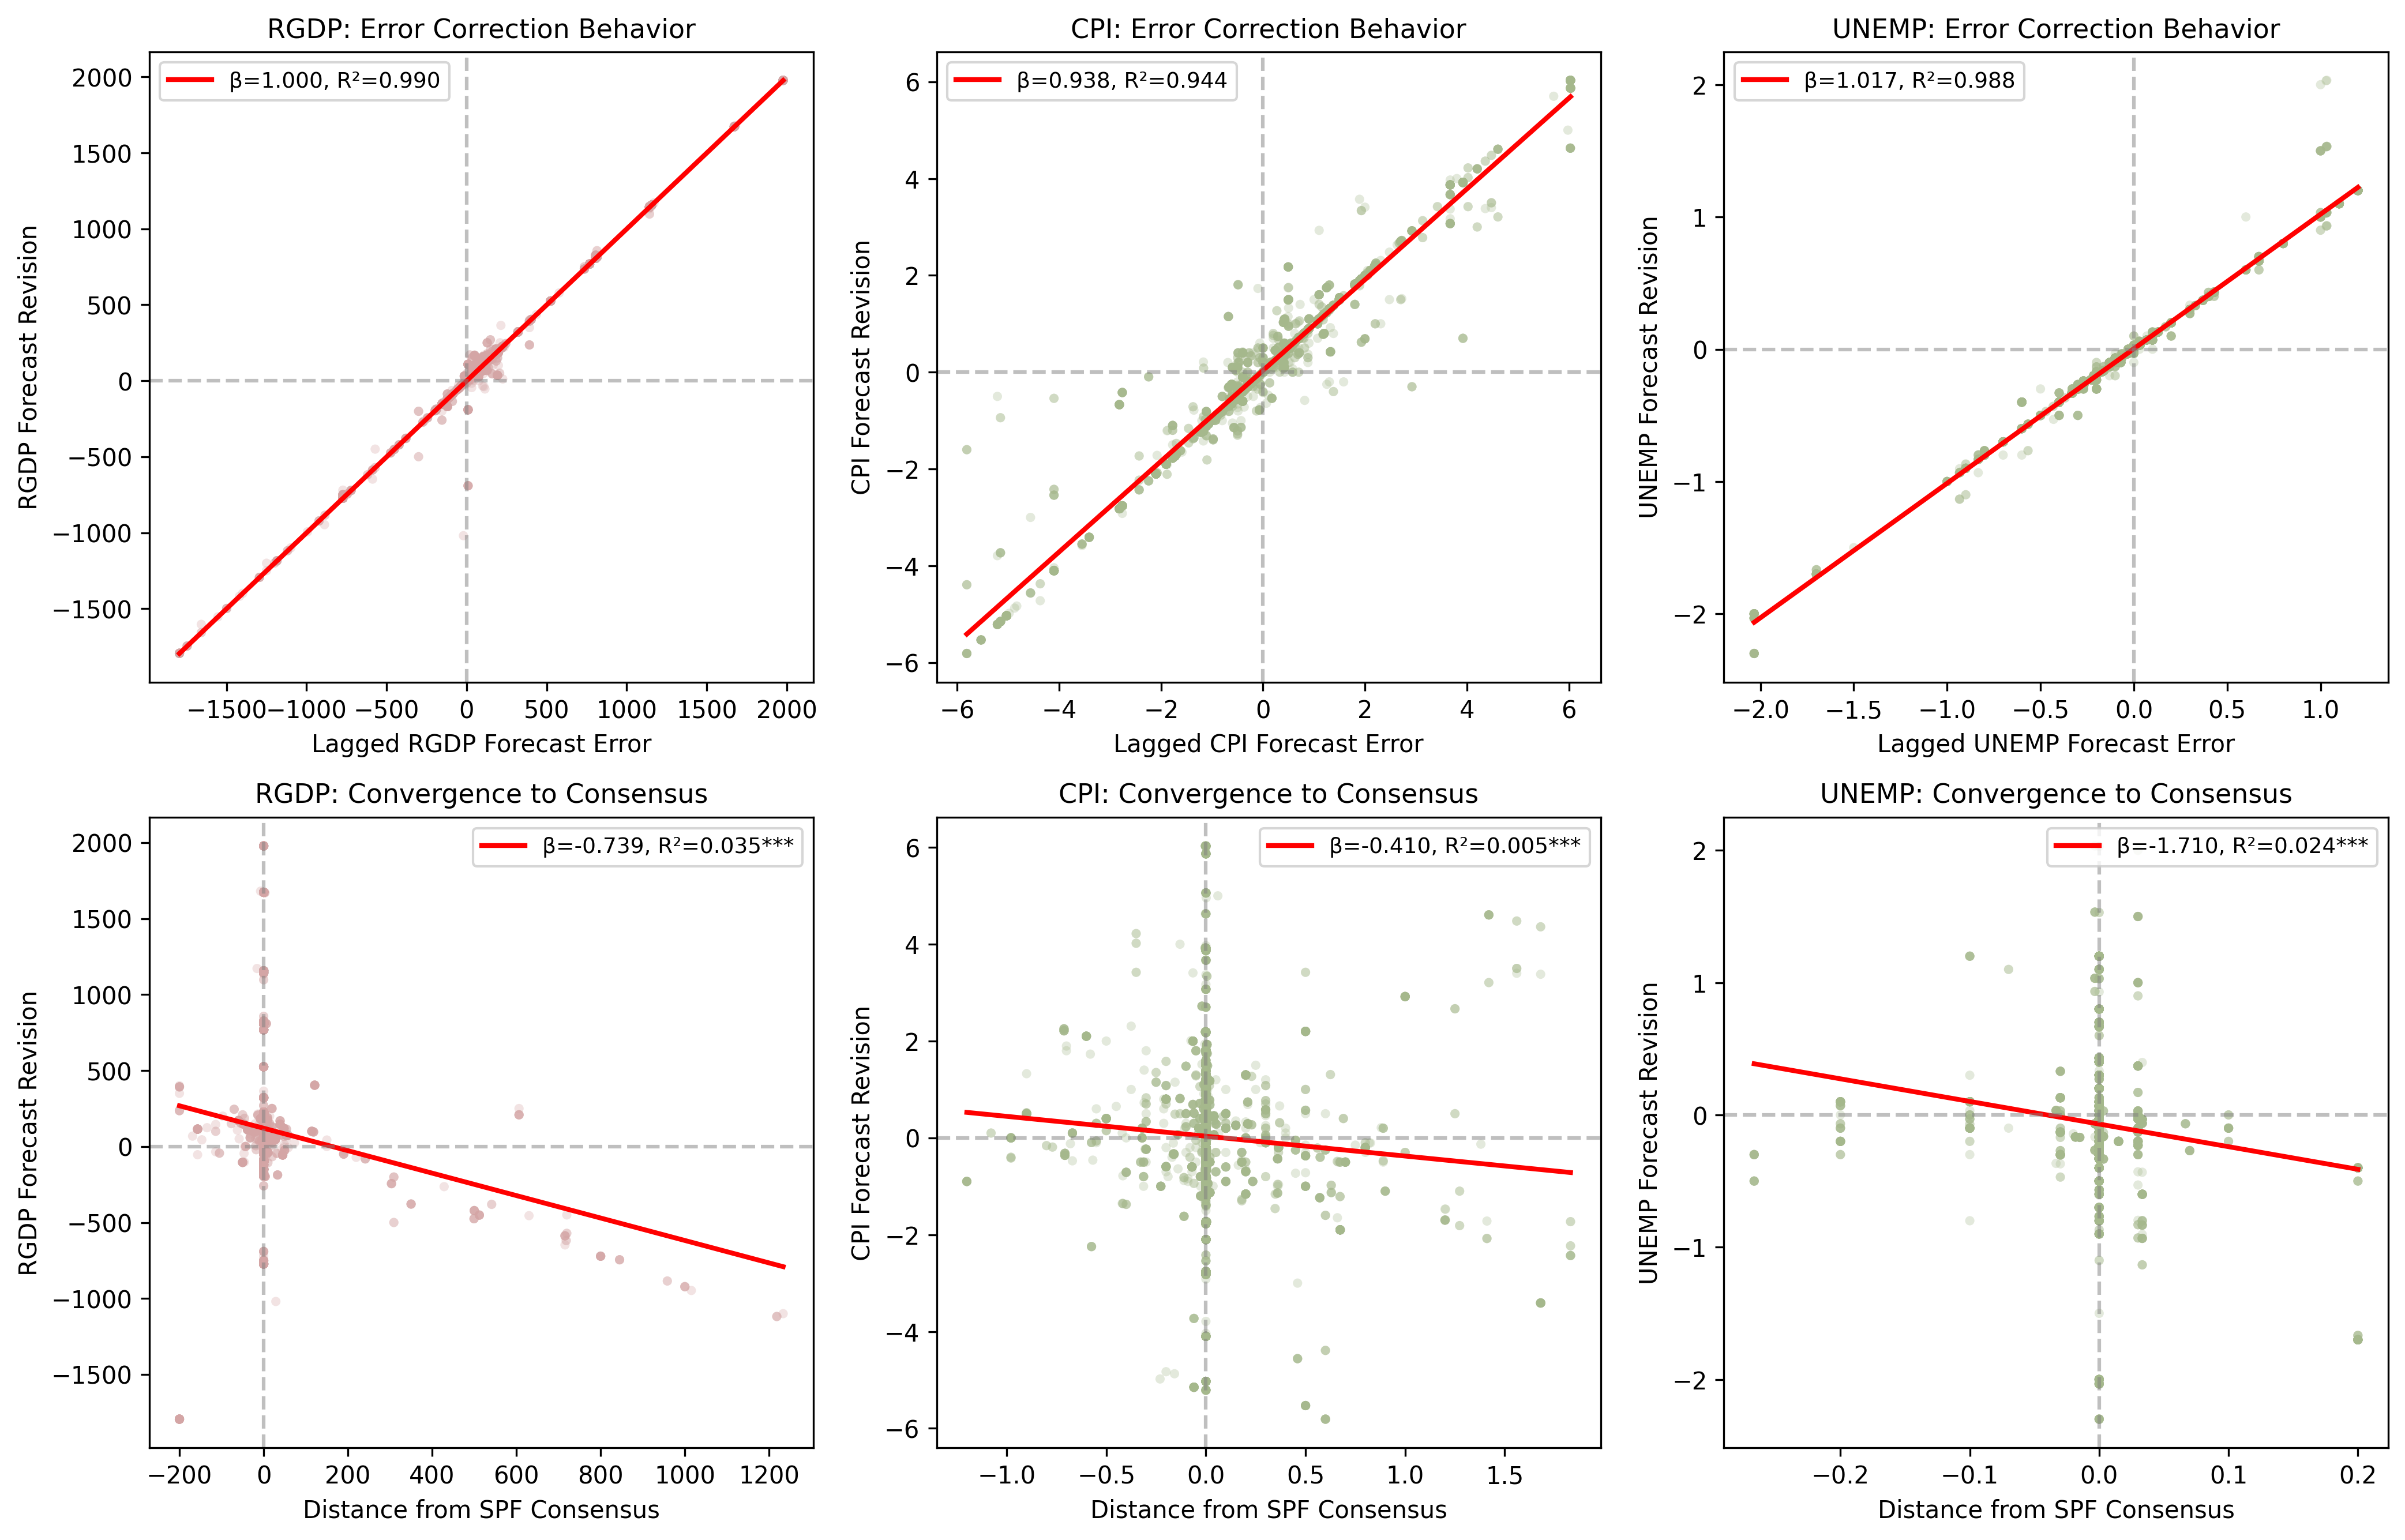
\includegraphics[width=\textwidth]{figures/figure9_revision_dynamics.png}
    \caption{Error Correction Behavior}
  \end{subfigure}
  
  \caption{Forecast Revision Dynamics}
  \label{fig:revisions}
  \vspace{5pt}
  \begin{minipage}{\textwidth}
    \raggedright
    \footnotesize \textit{Notes:} Panel A shows the relationship between forecast revisions (current forecast minus lagged forecast) and lagged forecast errors (lagged forecast minus realized value) for three variables. Each point represents a forecaster-quarter observation. The red lines show linear regression fits. Positive slopes indicate error correction: forecasters adjust future forecasts in response to past mistakes. Panel B shows the relationship between forecast revisions and the forecaster's distance from SPF consensus (lagged forecast minus lagged SPF median). Negative slopes indicate convergence toward consensus. Both panels restrict to consecutive forecast pairs (one quarter apart). Outliers beyond the 1st and 99th percentiles are excluded for visualization clarity.
  \end{minipage}
  \vspace{5pt}
\end{figure}

%%%%%%%%%%%%%%%%%%%%%%%%%%%%%%%%%%%%%%%%%%%%%%%%%%%%%%%%%%%%%%%%

\begin{figure}[t]
  \centering
  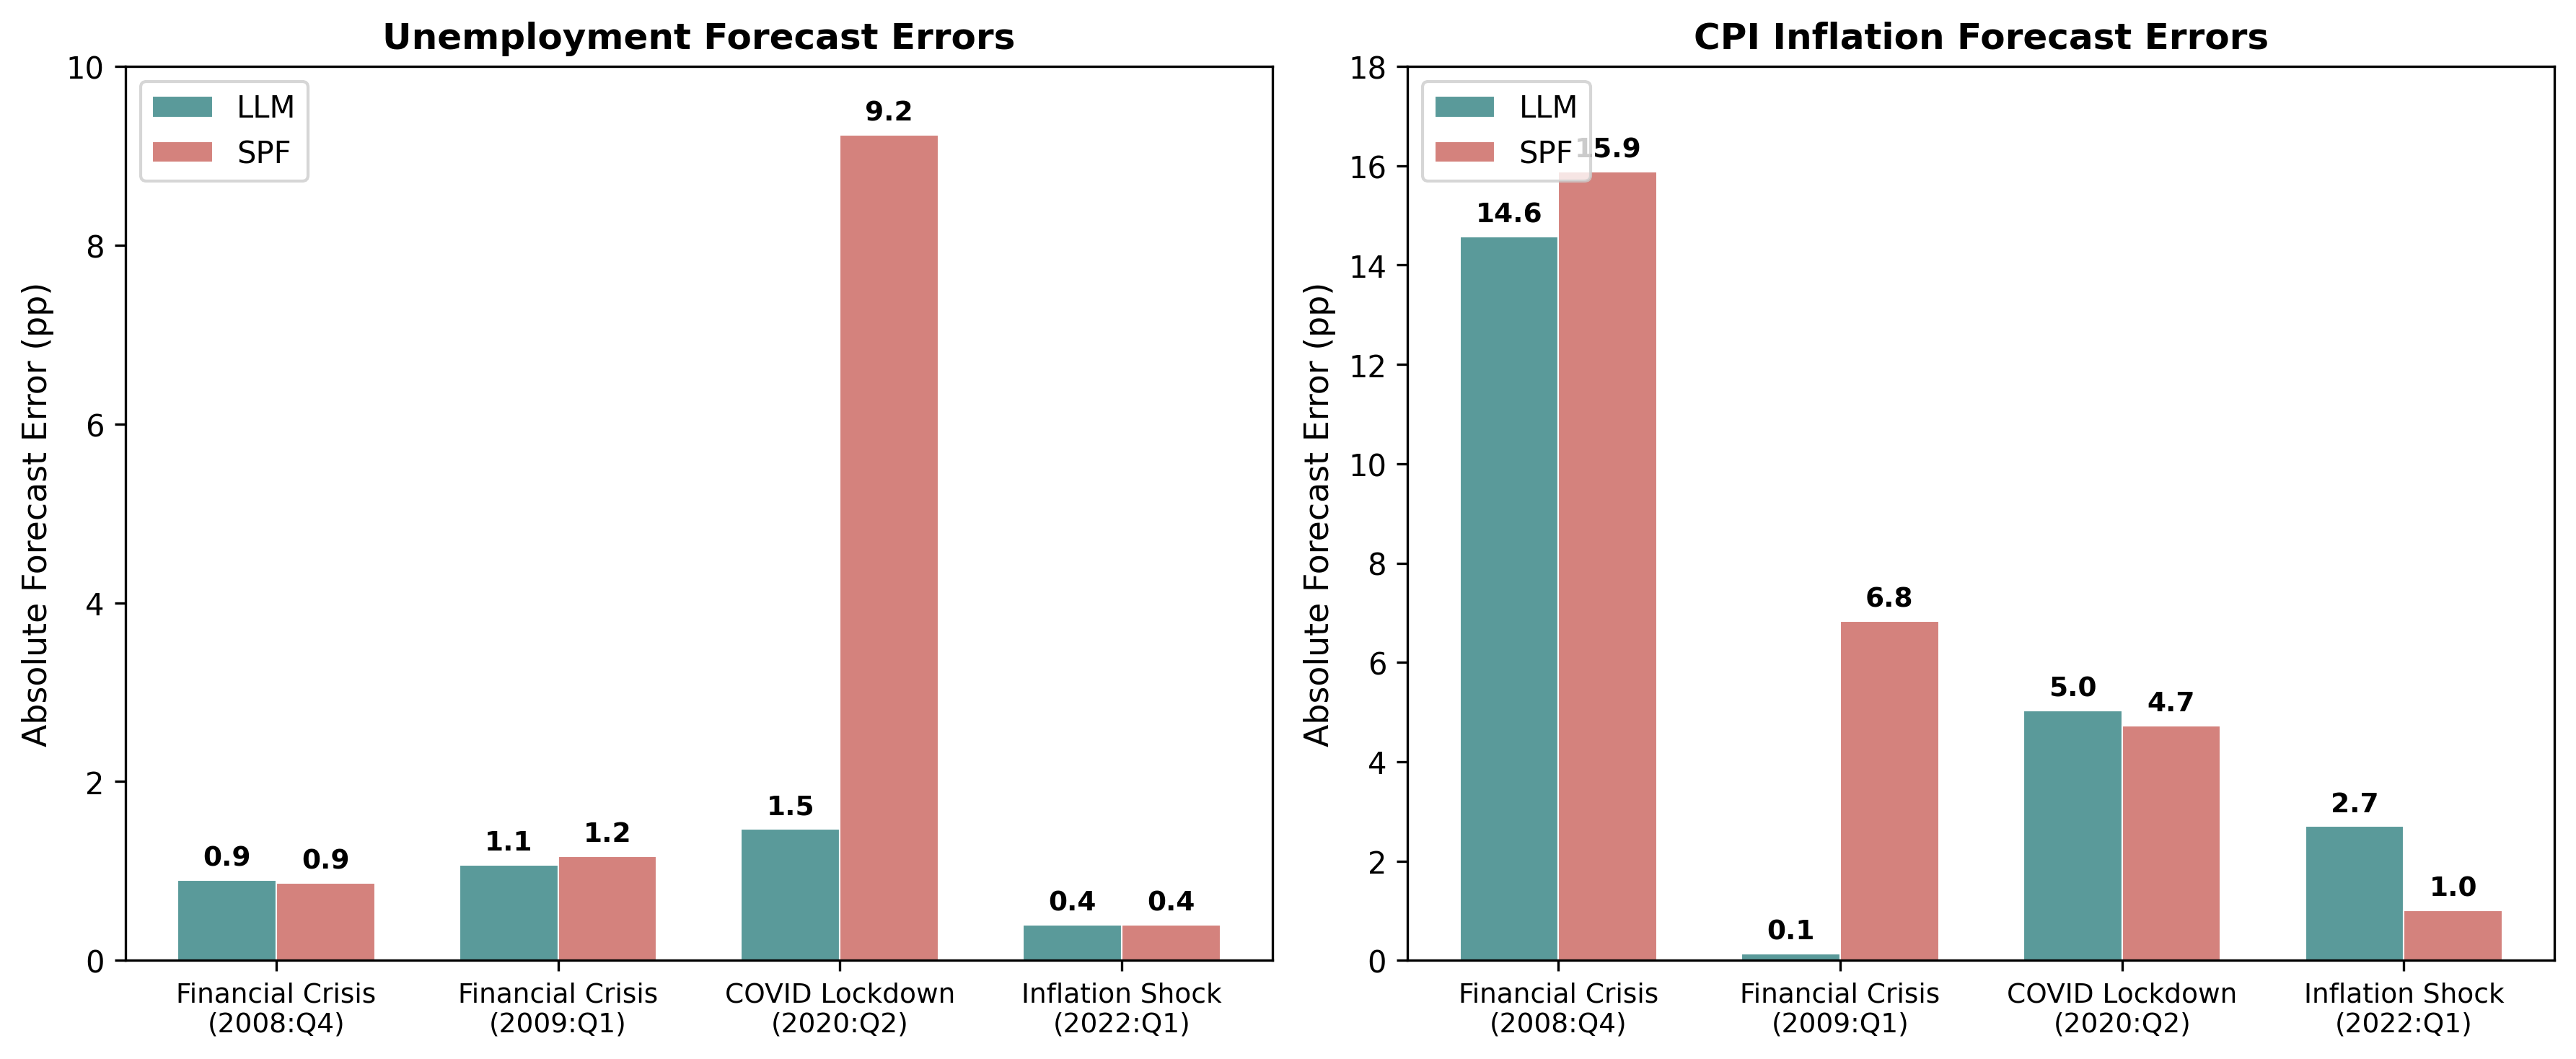
\includegraphics[width=\textwidth]{figures/figure_counterfactual_crisis.png}
  \caption{Forecaster Quality and Consensus Spreads Across Crisis Episodes}
  \label{fig:quality_counterfactual}
  \vspace{7pt}
  \begin{minipage}{\textwidth}
    \raggedright
    \footnotesize \textit{Notes:} The figure compares absolute forecast errors between LLM consensus (teal) and actual SPF consensus (coral) across four major crisis episodes. Left panel shows unemployment forecast errors in percentage points. Right panel shows CPI inflation forecast errors. The most striking result appears in the COVID lockdown quarter (2020:Q2): LLM forecasters predicted 14.5\% unemployment (error: 1.5 pp) while professional SPF forecasters predicted only 3.8\% (error: 9.2 pp); actual unemployment reached 13.0\%. For CPI during the financial crisis trough (2009:Q1), the LLM achieved near-perfect accuracy (error: 0.1 pp) compared to the SPF's substantial overshoot (error: 6.8 pp). These results suggest that LLM-based forecasts may provide valuable signals about the magnitude of unprecedented shocks, particularly for labor market variables.

  \end{minipage}
  \vspace{5pt}
\end{figure}
\end{comment}

%%%%%%%%%%%%%%%%%%%%%%%%%%%%%%%%%%%%%%%%%%%%%%%%%%%%%%%%%%%%%%%%
% TABLES
%%%%%%%%%%%%%%%%%%%%%%%%%%%%%%%%%%%%%%%%%%%%%%%%%%%%%%%%%%%%%%%%

\section*{Tables}
\begin{table}[H]
\centering
\caption{
    \textbf{Forecasting variables}
    \vspace{5pt}\\
    \footnotesize{The table lists the variables for which the SPF panel provides point forecasts and their definitions.}}
\label{tab:spf_variables_definitions}
\footnotesize
\begin{tabular}{p{1.8cm}p{14.2cm}}
\toprule
\textbf{Variable} & \textbf{Definition} \\
\hline
\multicolumn{2}{l}{{Section 1: U.S. Business Indicators}} \\
\hline
NGDP & Nominal Gross Domestic Product (GDP), levels, seasonally adjusted, annual rate, in billions USD. \\
PGDP & Gross Domestic Product (GDP) price index, chain weighted, seasonally adjusted, 2010 base year. \\
CPROF & Level of nominal corporate profits after tax excluding inventory valuation adjustment (IVA) and capital consumption adjustment (CCAdj). Seasonally adjusted, annual rate, in billions USD. \\
UNEMP & Civilian unemployment rate, levels, seasonally adjusted, percentage points. \\
EMP & Nonfarm payroll employment, seasonally adjusted, in thousands of jobs. \\
INDPROD & Industrial production index, seasonally adjusted, index, 2010 base year. \\
HOUSING & Housing starts, seasonally adjusted, annual rate, in millions. \\
TBILL & T-Bill rate, 3-month, levels, percentage points. \\
BOND AAA & AAA corporate bond yield, levels, percentage points.  \\
BOND BAA & BAA corporate bond yield, levels, percentage points.  \\
TBOND & Treasury bond rate, 10-year, levels, percentage points. \\
\hline
\multicolumn{2}{l}{\textbf{Section 2: Real GDP and Its Components}} \\
\hline
RGDP & Real Gross Domestic Product, seasonally adjusted, annual rate, 2010 base year. \\
RCONSUM & Real personal consumption expenditures, seasonally adjusted, annual rate, 2010 base year. \\
RNRESIN & Real nonresidential fixed investment, seasonally adjusted, annual rate, 2010 base year. \\
RRESINV & Real residential fixed investment, seasonally adjusted, annual rate, 2010 base year. \\
RFEDGOV & Real federal government consumption and gross investment, seasonally adjusted, annual rate, 2010 base year. \\
RSLGOV & Real state and local government consumption and gross investment, seasonally adjusted, annual rate, 2010 base year. \\
RCBI & Real change in private inventories, levels, chain-weighted real change in private inventories. Seasonally adjusted, annual rate, 2010 base year. \\
REXPORT & Real net exports of goods and services, levels, chain-weighted real net exports. Seasonally adjusted, annual rate, 2010 base year. \\
\hline
\multicolumn{2}{l}{\textbf{Section 3: CPI and PCE Inflation}} \\
\hline
CPI & Headline CPI inflation rate, seasonally adjusted, annual rate, percentage points. \\
CORECPI & Core CPI inflation rate, seasonally adjusted, annual rate, percentage points. \\
PCE & PCE inflation rate, headline chain-weighted, seasonally adjusted, annual rate, percentage points. \\
COREPCE & Core PCE inflation rate, core chain-weighted PCE inflation rate, seasonally adjusted, annual rate, percentage points. \\
\bottomrule
\end{tabular}
\end{table}
\clearpage

%%%%%%%%%%%%%%%%%%%%%%%%%%%%%%%%%%%%%%%%%%%%%%%%%%%%%%%%%%%%%%%%

\begin{table}[h!]
    \centering
    \footnotesize{
    \input{tables/characteristics_definitions.txt}
    }
    \caption{
    \textbf{Definitions of forecaster characteristics}
    \vspace{5pt}\\
    \footnotesize{The table shows definitions of forecaster characteristics, including inferred gender, affiliation, education, position, and public media engagement. The table is based on publicly available sources and may not fully capture the breadth of forecaster characteristics.}}
    \label{tab:forecaster_characteristics_definitions}
\end{table}
\clearpage

%%%%%%%%%%%%%%%%%%%%%%%%%%%%%%%%%%%%%%%%%%%%%%%%%%%%%%%%%%%%%%%%

\begin{table}[h!]
    \centering
    \footnotesize{
    \input{tables/descriptive_stats.txt}
    }
    \caption{
    \textbf{Descriptive statistics of forecast variables}
    \vspace{5pt}\\
    \footnotesize{The table shows the number of observations (N), mean, standard deviation (SD), skewness, kurtosis, median, minimum, maximum, and first-order autocorrelation coefficient (ACF(1)) of the data for each of the forecast variables.}}
    \label{tab:descriptive_stats}
\end{table}
\clearpage

\begin{comment}
\begin{table}[h!]
    \centering
    \footnotesize{
    \subfloat[One-quarter-ahead horizon]{
    \input{tables/test_moments_ai_against_spf_1.txt}}
    }
    \caption{
    \textbf{Differences in distributions between individual-level human and AI-generated SPF forecasts}
    \vspace{10pt}\\
    \footnotesize{The table shows the differences in distributional moments between individual-level human and AI-generated SPF forecasts for the horizons of (a) one quarter ahead and (b) four quarters ahead. The differences are tested for statistical significance using randomized tests based on 10,000 random draws. Significance levels: $^{\star}$ p-value$\leq$0.10, $^{\star\star}$ p-value$\leq$0.05, $^{\star\star\star}$ p-value$\leq$0.01.}
    \vspace{5pt}\\}
    \label{tab:distributional_tests_ai_spf}
    \emph{(Table continues on next page)}
\end{table}
\clearpage

\begin{table}[h!]\ContinuedFloat
    \centering
    \footnotesize{
    \subfloat[Four-quarter-ahead horizon]{\input{tables/test_moments_ai_against_spf_4.txt}}
    }
    \caption{
    \textbf{Differences in distributions between individual-level human and AI-generated SPF forecasts} \emph{(continued)}
    \vspace{5pt}\\}
    \label{tab:distributional_tests_ai_spf}
\end{table}
\clearpage
\end{comment}

%%%%%%%%%%%%%%%%%%%%%%%%%%%%%%%%%%%%%%%%%%%%%%%%%%%%%%%%%%%%%%%%

\begin{table}[h!]
    \centering
    \footnotesize{
    \input{tables/forecast_accuracy_ai_spf.txt}
    }
    \caption{
    \textbf{Forecast accuracy of human and AI-generated SPF forecasts}
    \vspace{5pt}\\
    \footnotesize{The table shows forecast accuracy reported as mean absolute errors computed as the average of absolute differences between realized values and median human and AI-generated SPF forecasts across survey quarters. Accuracy is reported for different forecast horizons, with 0, 1 and 4 denoting nowcast, one quarter and four quarters ahead, respectively. For each forecasting horizon, the table boldfaces the lowest MAE value between the AI and human surveys. The P-val column reports p-values and significance levels for randomized tests of the statistical significance of the difference between AI and human MAEs. The tests are based on 10,000 random draws. Significance levels: $^{\star}$ p-value$\leq$0.10, $^{\star\star}$ p-value$\leq$0.05, $^{\star\star\star}$ p-value$\leq$0.01.
}}
    \label{tab:forecastaccuracy_AI_SPF}
\end{table}
\clearpage

%%%%%%%%%%%%%%%%%%%%%%%%%%%%%%%%%%%%%%%%%%%%%%%%%%%%%%%%%%%%%%%%

\begin{table}[h!]
    \centering
    \footnotesize{
    \input{tables/forecast_accuracy_num_quarters_ai_spf.txt}
    }
    \caption{
    \textbf{Percentage survey quarters where AI is more accurate than the human SPF}
    \vspace{5pt}\\
    \footnotesize{The table shows forecast accuracy in terms of the percentage of survey quarters where the AI-generated SPF has lower forecast errors than the human SPF (Pct). Forecast errors are computed as the differences between realized values and median human and AI-generated SPF forecasts. Values are reported for different forecast horizons, with 0, 1 and 4 denoting nowcast, one quarter and four quarters ahead, respectively. The table boldfaces values above 50\%. The P-val column reports p-values and significance levels for randomized tests of the percentages being equal to 50\%. The tests are based on 10,000 random draws. Significance levels: $^{\star}$ p-value$\leq$0.10, $^{\star\star}$ p-value$\leq$0.05, $^{\star\star\star}$ p-value$\leq$0.01.
}}
    \label{tab:forecastaccuracy_AI_SPF_numquarters}
\end{table}
\clearpage

%%%%%%%%%%%%%%%%%%%%%%%%%%%%%%%%%%%%%%%%%%%%%%%%%%%%%%%%%%%%%%%%

\begin{table}[h!]
    \centering
    \footnotesize{
    \input{tables/forecast_accuracy_best_forecasters.txt}
    }
    \caption{
    \textbf{Forecast accuracy of best human and AI SPF forecasters}
    \vspace{10pt}\\
    \footnotesize{The table shows forecast accuracy reported as mean absolute errors computed as the average of absolute differences between realized values and the best human and AI-generated SPF forecasts across survey quarters. The best forecast is computed from the forecaster that achieves lowest average error across survey quarters. These best forecasters are identified separately for each variable and horizon. Accuracy is reported for different forecast horizons, with 0, 1 and 4 denoting nowcast, one quarter and four quarters ahead, respectively. For each forecasting horizon, the table boldfaces the lowest MAE value between the AI and human surveys. The P-val column reports p-values and significance levels for randomized tests of the statistical significance of the difference between AI and human MAEs. The tests are based on 10,000 random draws. Significance levels: $^{\star}$ p-value$\leq$0.10, $^{\star\star}$ p-value$\leq$0.05, $^{\star\star\star}$ p-value$\leq$0.01.
}}
    \label{tab:forecastaccacy_AI_SPF_best}
\end{table}
\clearpage

%%%%%%%%%%%%%%%%%%%%%%%%%%%%%%%%%%%%%%%%%%%%%%%%%%%%%%%%%%%%%%%%

\begin{comment}
\begin{table}[h!]
    \centering
    \footnotesize{
    \input{tables/accuracy_ai_against_spf_sector.txt}
    }
    \caption{
    \textbf{Forecast accuracy of human and AI SPF forecasters working in the financial sector}
    \vspace{10pt}\\
    \footnotesize{The table shows forecast accuracy reported as mean absolute errors computed as the average of absolute differences between realized values and the human and AI-generated SPF forecasts across survey quarters using only forecasters affiliated with financial firms.  Accuracy is reported for different forecast horizons, with 0, 1 and 2 denoting nowcast, one quarter and four quarters ahead, respectively. For each forecasting horizon, the table boldfaces the lowest MAE value between the AI and human surveys. The P-val column reports p-values and significance levels for randomized tests of the statistical significance of the difference between AI and human MAEs. The tests are based on 10,000 random draws. Significance levels: $^{\star}$ p-value$\leq$0.10, $^{\star\star}$ p-value$\leq$0.05, $^{\star\star\star}$ p-value$\leq$0.01.
}}
    \label{tab:forecastaccacy_AI_SPF_financial}
\end{table}
\clearpage
\end{comment}

%%%%%%%%%%%%%%%%%%%%%%%%%%%%%%%%%%%%%%%%%%%%%%%%%%%%%%%%%%%%%%%%

\begin{table}[h!]
\centering
\footnotesize
\begin{tabular}{lccccc}
\toprule
\textbf{Variable} & $\boldsymbol{\sigma_{h+1}}$ & $\boldsymbol{\sigma_{h+4}}$ & \textbf{Ratio} & \textbf{t-stat} & \textbf{N} \\
\midrule
\multicolumn{9}{l}{\textit{Panel A: Human}} \\[3pt]
CPI & 0.972 & 0.701 & 0.72 & $-6.82^{***}$ & 100 \\
UNEMP & 0.155 & 0.356 & 2.29 & $20.98^{***}$ & 100 \\
RGDP & 40.16 & 99.90 & 2.49 & $14.54^{***}$ & 100 \\
TBILL & 0.126 & 0.363 & 2.88 & $18.11^{***}$ & 100 \\
\midrule
\multicolumn{9}{l}{\textit{Panel B: AI}} \\[3pt]
CPI & 0.266 & 0.253 & 0.95 & $-0.64$ & 94 \\
UNEMP & 0.075 & 0.115 & 1.53 & $4.88^{***}$ & 72 \\
RGDP & 122.3 & 171.0 & 1.40 & $9.14^{***}$ & 91 \\
TBILL & 0.069 & 0.116 & 1.68 & $6.28^{***}$ & 73 \\
\bottomrule
\end{tabular}
\caption{\textbf{Cross-Sectional Disagreement by Forecast Horizon}\\
\vspace{10pt}\\
\footnotesize{Mean cross-sectional standard deviation at short (h+1) and long (h+4) horizons. Ratio = $\sigma_{h+4}/\sigma_{h+1}$. Positive t-statistics indicate greater disagreement at longer horizons. Paired t-tests (two-sided). Sample: 1999--2023. $^{***}p<0.01$.}}
\label{tab:horizon_dispersion}
\end{table}

%%%%%%%%%%%%%%%%%%%%%%%%%%%%%%%%%%%%%%%%%%%%%%%%%%%%%%%%%%%%%%%%

\begin{comment}
%%%% Forecaster Heterogeneity
\begin{table}[t]
  \centering
  \caption{Demographic Predictors of Forecast Heterogeneity}
  \label{tab:demographics}
  \begin{tabular}{lcccc}
  \toprule
  & \multicolumn{4}{c}{Fixed Effect (Deviation from Consensus)} \\
  \cmidrule{2-5}
  & RGDP & PGDP & CPI & UNEMP \\
  \midrule
  \multicolumn{5}{l}{\textit{Panel A: Affiliation Type}} \\
  Banking & 0.768 & $0.018^{***}$ & 0.002 & $-0.001$ \\
  & (9.82) & (0.006) & (0.088) & (0.007) \\
  Academia & $-0.116$ & $-0.017^{***}$ & 0.003 & 0.002 \\
  & (10.45) & (0.006) & (0.092) & (0.009) \\
  \midrule
  \multicolumn{5}{l}{\textit{Panel B: Education}} \\
  Ph.D. & $-0.595^{**}$ & $-0.003^{**}$ & 0.002 & $-0.001$ \\
  & (0.275) & (0.001) & (0.011) & (0.001) \\
  No Ph.D. & $4.842^{**}$ & $0.021^{**}$ & 0.003 & $-0.001$ \\
  & (1.313) & (0.008) & (0.016) & (0.001) \\
  \midrule
  Observations & 121 & 121 & 121 & 121 \\
  Significant effects & 1 & 2 & 0 & 0 \\
  \bottomrule
  \end{tabular}
  \begin{tablenotes}
   {\footnotesize
  The table reports mean fixed effects by forecaster characteristics. Fixed effects are calculated as the time-series average of each forecaster's deviation from quarterly consensus. Panel A compares banking forecasters (commercial and investment banks) to academic forecasters (universities, research institutions, think tanks). Panel B compares forecasters with and without doctoral degrees. Standard errors in parentheses. Sample restricted to forecasters with at least 10 observations. RGDP and PGDP measured in billions (2012\$) and index points, respectively; CPI and UNEMP measured in percentage points. Three significant demographic effects emerge: banking forecasters predict higher GDP price levels than academics; Ph.D. holders forecast lower real GDP growth and lower price levels than non-Ph.D. forecasters. $^{*}p<0.10$, $^{**}p<0.05$, $^{***}p<0.01$.}
  \end{tablenotes}
\end{table}
\end{comment}
\clearpage

%%%%%%%%%%%%%%%%%%%%%%%%%%%%%%%%%%%%%%%%%%%%%%%%%%%%%%%%%%%%%%%%

\thispagestyle{empty}
\begin{table}[h!]
    \centering
    \footnotesize{
    \input{tables/forecast_accuracy_generic.txt}
    }
    \caption{
    \textbf{Relative accuracy of AI forecasts with fewer prompt inputs}
    \vspace{10pt}\\
    \footnotesize{The table shows the accuracy of AI forecasts generated by prompts that provide less information relative to the accuracy of baseline AI forecasts (ratio). Forecast accuracy is computed as mean absolute errors, i.e., the average of absolute differences between realized values and the median human or AI-generated SPF forecasts across survey quarters. The ``Generic'' forecast uses a prompt that does not provide forecaster characteristics, but does provide real-time data and past median SPF forecasts. The ``Generic, w/o real-time data'' excludes both forecaster characteristics and real-time data from the prompt. ``Generic, w/o real-time data, w/o past SPF data'' excludes all data from the prompt including forecaster characteristics, real-time data, and past median SPF forecasts. Finally ``Recall'' prompts the model to recall values from the training data rather than forecasting values. Values exceeding one (boldfaced) indicate less accuracy compared with the baseline AI forecaster seeded with forecaster characteristics, real-time data, and past median SPF forecasts. Randomized tests evaluate whether values are significantly different from one. The tests are based on 10,000 random draws. Significance levels: $^{\star}$ p-value$\leq$0.10, $^{\star\star}$ p-value$\leq$0.05, $^{\star\star\star}$ p-value$\leq$0.01.
    }}
    \label{tab:MAEs_forecastaccuracy_generic}
\end{table}

%%%%%%%%%%%%%%%%%%%%%%%%%%%%%%%%%%%%%%%%%%%%%%%%%%%%%%%%%%%%%%%%

\begin{table}[h!]
    \centering
    \footnotesize{
    	\begin{tabular}{p{5cm}C{1.5cm}L{4.5cm}C{1.5cm}C{1.5cm}}
		\toprule
		Event & Event Date & Relevant Variables & \multicolumn{2}{c}{Average Z-Score} \\
        \cmidrule{4-5}
        &&& Relevant Variables & All Variables \\
		\hline
		9/11 Attacks & 2001-09-11 (27 days) & RGDP, UNEMP, CPI, TBILL, TBOND & 0.28 & 0.01 \\
		Lehman Brothers Collapse & 2008-09-15 (39 days) & RGDP, UNEMP, CPI, TBILL, TBOND, HOUSING & 1.49 & 0.49 \\
		Flash Crash & 2010-05-06 (-5 days) & RGDP, CPI & 0.00 & -0.12 \\
		S\&P Downgrade of U.S. Debt & 2011-08-05 (-3 days) & TBILL, TBOND, RGDP & 0.26 & -0.06 \\
		COVID-19 Pandemic Declaration & 2020-03-11 (29 days) & RGDP, UNEMP, CPI, HOUSING, INDPROD & 1.19 & 0.77 \\
		Russia-Ukraine War & 2022-02-24 (17 days) & RGDP, CPI, TBILL, TBOND & 0.72 & 0.29 \\
		Silicon Valley Bank Collapse & 2023-03-10 (31 days) & RGDP, UNEMP, TBILL, TBOND & -0.20 & -0.09 \\
		\bottomrule
	   \end{tabular}
    }
    \caption{
    \textbf{AI Forecast Performance During Unexpected Events}
    \vspace{10pt}\\
    \footnotesize{The table shows the performance of AI forecasters during seven unexpected events occurring immediately before or after the deadline of the SPF survey (days after survey deadline denoted in parenthesis after the event date). The table reports average Z-scores, measuring the difference between the event-period forecast error and the mean forecast error across the full sample, divided by the standard deviation of the full-sample forecast error. Z-scores near zero indicate typical forecast difficulty, while highly negative values (e.g., <-1) would indicate suspiciously accurate predictions suggesting look-ahead bias. The Z-scores are averaged across the relevant variables for each event and across all variables.
    }}
    \label{tab:unexpected_events}
\end{table}

%%%%%%%%%%%%%%%%%%%%%%%%%%%%%%%%%%%%%%%%%%%%%%%%%%%%%%%%%%%%%%%%
\clearpage
\begin{table}[]
    \centering
    \caption{\textbf{AI Forecast Error Regressions on Knowledge Cut-Off Dummy Variable}
    \vspace{10pt}\\
    {\footnotesize 
    The table reports OLS regressions of absolute forecast errors of AI forecasters at the one-quarter ahead horizon on a dummy variable, $I_{t>\text{Oct 2023}}$, that takes value one after the LLM knowledge cut-off date (October 2023). $^{***}p<0.001$, $^{**}p<0.01$, $^{*}p<0.05$. Standard errors in parentheses.}
    }
    \label{tab:cutoff_regressions}
    \footnotesize
    \begin{tabular}{lcccc}
    \toprule
    & RGDP & UNEMP & CPI & TBILL \\
    \hline
    Intercept & 366.06*** & 0.714*** & 2.135*** & 0.652*** \\
    & (65.43) & (0.141) & (0.210) & (0.076) \\
    $I_{t>\text{Oct 2023}}$ & 715.56* & $-$0.539 & $-$1.323 & $-$0.137 \\
    & (340.01) & (0.732) & (1.091) & (0.397) \\
    \hline
    Observations & 108 & 108 & 108 & 108 \\
    $R^2$ & 0.040 & 0.005 & 0.014 & 0.001 \\
    \bottomrule
    \end{tabular}
\end{table}

%%%%%%%%%%%%%%%%%%%%%%%%%%%%%%%%%%%%%%%%%%%%%%%%%%%%%%%%%%%%%%%%

\begin{table}[t]
\centering
\caption{\textbf{Forecast Revision Regressions: Human vs AI}
\vspace{10pt}\\
{\footnotesize 
The table reports OLS regressions of forecast revisions on lagged forecast errors (Error Correction) and distance from SPF consensus (Consensus Tracking). Revision$_{it}$ is the change in forecaster $i$'s nowcast from $t-1$ to $t$. SPF regressions use individual forecaster microdata from the Philadelphia Fed (1999--2023). Robust standard errors in parentheses. $^{***}p<0.01$.}
}
\label{tab:revision_regressions}
\footnotesize
\begin{tabular}{lcccccccc}
\toprule
& \multicolumn{4}{c}{\textbf{Error Correction}} & \multicolumn{4}{c}{\textbf{Consensus Tracking}} \\
\cmidrule(lr){2-5} \cmidrule(lr){6-9}
& RGDP & CPI & UNEMP & TBILL & RGDP & CPI & UNEMP & TBILL \\
\midrule
\multicolumn{9}{l}{\textit{Panel A: Human}} \\[3pt]
Lagged Error$_{i,t-1}$ & $0.981^{***}$ & $0.881^{***}$ & $0.956^{***}$ & $0.975^{***}$ & & & & \\
 & (0.008) & (0.016) & (0.007) & (0.008) & & & & \\[3pt]
Distance from Consensus$_{i,t-1}$ & & & & & $-0.612^{***}$ & $-0.690^{***}$ & $-0.868^{***}$ & $-0.296^{***}$ \\
 & & & & & (0.134) & (0.035) & (0.064) & (0.102) \\[3pt]
Observations & 3,437 & 3,452 & 3,615 & 3,309 & 3,437 & 3,452 & 3,615 & 3,309 \\
$R^2$ & 0.941 & 0.636 & 0.911 & 0.922 & 0.015 & 0.140 & 0.072 & 0.004 \\
\midrule
\multicolumn{9}{l}{\textit{Panel B: AI}} \\[3pt]
Lagged Error$_{i,t-1}$ & $0.610^{***}$ & $0.443^{***}$ & $0.647^{***}$ & $0.594^{***}$ & & & & \\
 & (0.028) & (0.018) & (0.008) & (0.008) & & & & \\[3pt]
Distance from Consensus$_{i,t-1}$ & & & & & $-1.016^{***}$ & $-0.693^{***}$ & $-0.510^{***}$ & $-1.143^{***}$ \\
 & & & & & (0.004) & (0.017) & (0.049) & (0.011) \\[3pt]
Observations & 5,188 & 5,188 & 5,188 & 5,188 & 5,188 & 5,188 & 5,188 & 5,188 \\
$R^2$ & 0.568 & 0.354 & 0.946 & 0.827 & 0.776 & 0.551 & 0.086 & 0.716 \\
\bottomrule
\end{tabular}
\end{table}
\clearpage

%%%%%%%%%%%%%%%%%%%%%%%%%%%%%%%%%%%%%%%%%%%%%%%%%%%%%%%%%%%%%%%%

\begin{comment}
\begin{table}[t]
\centering
\caption{\textbf{Counterfactual: Human vs AI Consensus During Major Economic Crises}
\vspace{10pt}\\
{\footnotesize 
The table compares LLM consensus forecasts (median of simulated panel) to actual SPF consensus (median of professional forecasters) during major economic crises. Bold values indicate lower absolute forecast error. The COVID lockdown result is striking: LLM forecasters predicted 14.5\% unemployment while professional forecasters predicted only 3.8\%; actual unemployment reached 13.0\%.}
}
\label{tab:counterfactual_crisis}
\footnotesize
\begin{tabular}{lcccccc}
\toprule
& \multicolumn{3}{c}{Unemployment (\%)} & \multicolumn{3}{c}{CPI Inflation (\%)} \\
\cmidrule(lr){2-4} \cmidrule(lr){5-7}
Crisis & Actual & AI & Human & Actual & AI & Human \\
\midrule
Financial Crisis (2008:Q4) & 6.9 & 6.0 & 6.0 & $-9.2$ & 5.4 & 6.7 \\
Financial Crisis (2009:Q1) & 8.1 & 7.0 & 6.9 & $-2.4$ & $-2.5$ & $-9.2$ \\
COVID Lockdown (2020:Q2) & 13.0 & 14.5 & 3.8 & $-3.5$ & 1.5 & 1.2 \\
Inflation Shock (2022:Q1) & 3.8 & 4.2 & 4.2 & 9.2 & 6.5 & 8.2 \\
\midrule
\multicolumn{7}{l}{\textit{Absolute Forecast Error (pp)}} \\
Financial Crisis (2008:Q4) & --- & 0.9 & 0.9 & --- & \textbf{14.6} & 15.9 \\
Financial Crisis (2009:Q1) & --- & \textbf{1.1} & 1.2 & --- & \textbf{0.1} & 6.8 \\
COVID Lockdown (2020:Q2) & --- & \textbf{1.5} & 9.2 & --- & 5.0 & \textbf{4.7} \\
Inflation Shock (2022:Q1) & --- & 0.4 & 0.4 & --- & 2.7 & \textbf{1.0} \\
\bottomrule
\end{tabular}
\end{table}
\clearpage
\end{comment}

%%%%%%%%%%%%%%%%%%%%%%%%%%%%%%%%%%%%%%%%%%%%%%%%%%%%%%%%%%%%%%%%

\begin{table}[!htbp]
\centering
\footnotesize
\begin{tabular}{lrccccccc}
\toprule
& & \multicolumn{4}{c}{\textbf{Detailed Categories}} & & \multicolumn{2}{c}{\textbf{ECB Aggregation}} \\
\cmidrule(lr){3-6} \cmidrule(lr){8-9}
\textbf{Period} & \textbf{N} & Mechanical & Policy & Model & Event & & Model-Based & Judgment-Based \\
\midrule
Normal & 4,626 & 98.6\% & 55.2\% & 86.7\% & 19.7\% & & 99.6\% & 63.3\% \\
Financial Crisis & 346 & 84.7\% & 34.4\% & 37.6\% & 82.4\% & & 88.4\% & 87.6\% \\
COVID-19 & 204 & 72.1\% & 59.8\% & 26.5\% & 77.0\% & & 72.5\% & 79.9\% \\
Inflation Shock & 212 & 85.4\% & 87.3\% & 97.2\% & 30.2\% & & 98.1\% & 87.7\% \\
\bottomrule
\end{tabular}
\caption{\textbf{Reasoning Categories by Economic Period}\\
\vspace{5pt}\\
\footnotesize{Percentage of forecaster responses containing each reasoning type. Categories are non-exclusive. \textit{Detailed categories}: Mechanical (trends, historical patterns, mean-reversion); Policy (Fed actions, fiscal/monetary policy); Model (economic theory such as Phillips curve, Okun's law); Event (specific shocks or crises). \textit{ECB aggregation}: Following ECB methodology, Model-Based combines Mechanical $\cup$ Model; Judgment-Based combines Policy $\cup$ Event. All differences between crisis and normal periods are statistically significant ($p < 0.001$).}}
\label{tab:reasoning_categories}
\end{table}
\clearpage

%%%%%%%%%%%%%%%%%%%%%%%%%%%%%%%%%%%%%%%%%%%%%%%%%%%%%%%%%%%%%%%%
% PROMPTS
%%%%%%%%%%%%%%%%%%%%%%%%%%%%%%%%%%%%%%%%%%%%%%%%%%%%%%%%%%%%%%%%
\section*{Prompts}
\setcounter{figure}{0}
\renewcommand{\figurename}{Prompt}

\begin{figure}[h!]
    \centering
    \caption{\textbf{Baseline Prompt}}
    \label{prmpt:baseline} 
    \begin{tcolorbox}[colback=gray!10, colframe=gray!10, width=\textwidth]
    \scriptsize
    \begin{Verbatim}[commandchars=\\\{\}]
    
    You are a participant on a panel of Survey of Professional Forecasters. 
    Your name is [\textcolor{blue}{name}], you graduated from [\textcolor{blue}{alma mater}] with a [\textcolor{blue}{education}] around [\textcolor{blue}{graduation year}]. 
    Today, you work as [\textcolor{blue}{title}] at [\textcolor{blue}{affiliation}]. It's [\textcolor{blue}{affiliation type}] organization.
    Your organization is based in [\textcolor{blue}{company_location}]. You are originally from [\textcolor{blue}{country_origin}]. 
    [\textcolor{blue}{social media status}].
                
    We are in [\textcolor{blue}{date_q}]. You are about to fill out the forecast form for [\textcolor{blue}{date_q}]. Using only the 
    information available to you as of [\textcolor{blue}{release_date}], please provide your best numeric forecasts for 
    the following variables: [\textcolor{blue}{variable_definitions}]. 
    Do this for the following quarters: t (current quarter), t+1, t+2, t+3, t+4, and annual forecasts 
    for this and next year (annual averages).
    
    You have the most recent real-time data on key macroeconomics variables available to you 
    (from [\textcolor{blue}{prev_quarter}]): [\textcolor{blue}{real_time_data}]. 
    
    The forecasts made by the SPF panel during the previous quarter ([\textcolor{blue}{prev_quarter}]) were as follows 
    (for t, t+1, t+2, t+3, t+4; where t is the current quarter): [\textcolor{blue}{variable_forecasts_text}].
    
    Do not incorporate any data that was not available to you beyond the current date. 
    Do consider all relevant information on the broad economic conditions and current Federal Reserve 
    actions (up to, but not beyond [\textcolor{blue}{release_date}]). 
    Use available information, and your professional judgement and experience. 
    Your forecast is anonymous.
    
    For each variable, provide the forecasts as a sequence of numerical values in the following format:
    [\textcolor{blue}{variable_name}]: t, t+1, t+2, t+3, t+4, this year's avg, next year's avg
    
    Please only provide your forecasts in this format.

    \end{Verbatim}
    \end{tcolorbox}
\end{figure}
\clearpage

\begin{comment}
Please provide the reasoning behind your forecast. Please limit your response to 1-2 sentences.

Please provide a brief explanation for your forecast in 1-2 sentences.

To what extent are your point forecasts model or judgment-based? (By 'model' we mean any mathematical representation of relationships between economic variables; by "judgment" we mean experience and intuition.)

Please select one of the following options:
1. Essentially judgement-based
2. Model-based with judgemental adjustments
3. Essentially model-based

Please respond with the number (1, 2, or 3) and optionally a brief comment.
\end{comment}

\begin{figure}[h!]
    \centering
    \caption{\textbf{Prompt for a generic forecaster}
    \vspace{5pt}\\
    \footnotesize{This prompt is used to generate AI forecasts for a generic forecaster, i.e., without including forecaster characteristics. The input variables are highlighted in brackets and blue text and consist of real-time data, previous forecasts, survey dates, and forecasting variable names.} 
    \vspace{5pt}
    }
    \label{prmpt:generic_forecaster} 

\begin{tcolorbox}[colback=gray!10, colframe=gray!10, width=\textwidth]
\scriptsize
\begin{Verbatim}[commandchars=\\\{\}]

You are a professional economic forecaster participating in the Survey of Professional Forecasters. 
You have expertise in macroeconomic analysis and forecasting. Use your professional judgment and the 
data provided to make your forecasts.
            
We are in [\textcolor{blue}{date_q}]. You are about to fill out the forecast form for [\textcolor{blue}{date_q}]. Using only the 
information available to you as of [\textcolor{blue}{release_date}], please provide your best numeric forecasts for: 
[\textcolor{blue}{variable_definitions}]. 

For quarters: t (current), t+1, t+2, t+3, t+4, and annual averages for this year and next year. 

Real-time data available (from [\textcolor{blue}{prev_quarter}]): [\textcolor{blue}{real_time_data}]. 

Previous SPF panel forecasts ([\textcolor{blue}{prev_quarter}], for t, t+1, t+2, t+3, t+4): [\textcolor{blue}{variable_forecasts_text}]. 

Do not incorporate any data beyond [\textcolor{blue}{release_date}]. Consider all relevant economic conditions and 
Federal Reserve actions up to [\textcolor{blue}{release_date}]. 

Format your response as: [\textcolor{blue}{variable_name}]: t, t+1, t+2, t+3, t+4, this year's avg, next year's avg

Provide only numerical values.
\end{Verbatim}
\end{tcolorbox}
\end{figure}
\clearpage


\begin{figure}[h!]
    \centering
    \caption{\textbf{Prompt for a generic forecaster and no real-time data}
    \vspace{5pt}\\
    \footnotesize{This prompt is used to generate AI forecasts for a generic forecaster, i.e., without including forecaster characteristics. The input variables are highlighted in brackets and blue text and consist of previous forecasts, survey dates, and forecasting variable names.} 
    \vspace{5pt}
    }

    \label{prmpt:generic_forecaster_norealtime} 

    \begin{tcolorbox}[colback=gray!10, colframe=gray!10, width=\textwidth]
\scriptsize
\begin{Verbatim}[commandchars=\\\{\}]

You are a professional economic forecaster participating in the Survey of Professional Forecasters. 
You have expertise in macroeconomic analysis and forecasting. Use your professional judgment and the 
data provided to make your forecasts.

We are in [\textcolor{blue}{date_q}]. You are about to fill out the forecast form for [\textcolor{blue}{date_q}]. Using only the 
information available to you as of [\textcolor{blue}{release_date}], please provide your best numeric forecasts for: 
[\textcolor{blue}{variable_definitions}]. 

For quarters: t (current), t+1, t+2, t+3, t+4, and annual averages for this year and next year. 

Previous SPF panel forecasts ([\textcolor{blue}{prev_quarter}]): [\textcolor{blue}{var_forecasts_text}]. 

Do not incorporate any data beyond [\textcolor{blue}{release_date}]. Consider all relevant economic conditions and 
Federal Reserve actions up to [\textcolor{blue}{release_date}]. 

Format your response as: [\textcolor{blue}{variable_name}]: t, t+1, t+2, t+3, t+4, this year's avg, next year's avg

Provide only numbers.
\end{Verbatim}
\end{tcolorbox}
\end{figure}
\clearpage



\begin{figure}[h!]
    \centering
    \caption{\textbf{Prompt for a generic forecaster and no data}
    \vspace{5pt}\\
    \footnotesize{This prompt is used to generate AI forecasts for a generic forecaster, i.e., without including forecaster characteristics or any data on economic variables. The input variables are highlighted in brackets and blue text and consist of only survey dates, and forecasting variable names.} 
    \vspace{5pt}
    }

    \label{prmpt:generic_forecaster_nodata} 

\begin{tcolorbox}[colback=gray!10, colframe=gray!10, width=\textwidth]
\scriptsize
\begin{Verbatim}[commandchars=\\\{\}]

You are a professional economic forecaster participating in the Survey of Professional Forecasters. 
You have expertise in macroeconomic analysis and forecasting. Use your professional judgment and the
data provided to make your forecasts.

We are in [\textcolor{blue}{date_q}]. You are about to fill out the forecast form for [\textcolor{blue}{date_q}]. Using only the 
information available to you as of [\textcolor{blue}{release_date}], please provide your best numeric forecasts for: 
[\textcolor{blue}{variable_definitions}]. 

For quarters: t (current), t+1, t+2, t+3, t+4, and annual averages for this year and next year. 

Do not incorporate any data beyond [\textcolor{blue}{release_date}]. Consider all relevant economic conditions and 
Federal Reserve actions up to [\textcolor{blue}{release_date}]. 

Format your response as: [\textcolor{blue}{variable_name}]: t, t+1, t+2, t+3, t+4, this year's avg, next year's avg.

Provide only numbers.
\end{Verbatim}
\end{tcolorbox}
\end{figure}

\begin{figure}[h!]
    \centering
    \caption{\textbf{Prompt for recall task}
    \vspace{5pt}\\
    \footnotesize{This prompt is used to have the model recall specific values of economic variables.} 
    \vspace{5pt}
    }

    \label{prmpt:recall} 

    \begin{tcolorbox}[colback=gray!10, colframe=gray!10, width=\textwidth]
\scriptsize
\begin{Verbatim}[commandchars=\\\{\}]

You are a professional forecaster participating in the Survey of Professional Forecasters (SPF).

Please provide your best guess for the requested variables.
            
We are in [\textcolor{blue}{date_q}]. What is the value for the following variables: [\textcolor{blue}{variable_data}] 
for this quarter: [\textcolor{blue}{date_q}]

\end{Verbatim}
\end{tcolorbox}
\end{figure}
\clearpage

%[Add Supplemental Matricals page]
%%%%%%%%%%%%%%%%%%%%%%%%%%%%%%%%%%%%%%%%%%%%%%%%%%%%%%%%%%%%%%%%
% APPENDICES
%%%%%%%%%%%%%%%%%%%%%%%%%%%%%%%%%%%%%%%%%%%%%%%%%%


\newpage\clearpage
\appendix
\renewcommand{\headrulewidth}{0pt}
\renewcommand{\footrulewidth}{0pt}
\lhead{}
\setcounter{figure}{0}
\renewcommand{\figurename}{Figure}
\renewcommand{\theequation}{\Alph{section}.\arabic{equation}}
\renewcommand*\thetable{\Alph{section}.\arabic{table}}
\renewcommand*\thefigure{\Alph{section}.\arabic{figure}}
\renewcommand{\thepage}{A\arabic{page}} 
\setcounter{page}{1}
%\setcounter{footnote}{0}
\fancyhead{}
\pagestyle{fancy}
%\fancyfoot[C]{{\footnotesize \textbf{--\,A \thepage\,--}}}


\begin{center}
        \vspace*{4cm}\Large{\textbf{Online Appendix for\\[2ex]
        ``Simulating the Survey of Professional Forecasters'' }}\vspace{.81cm}

        \large{\textit{} }

%\vspace{2cm}\textbf{Abstract}\vspace{.051cm}
\end{center}
\doublespacing{\textit{This Internet Appendix provides additional material on the data, methodology, and some robustness exercises related to the main text. }}

\newpage\clearpage

\section{Descriptive Figures}

\begin{figure}[h!]
    \centering
    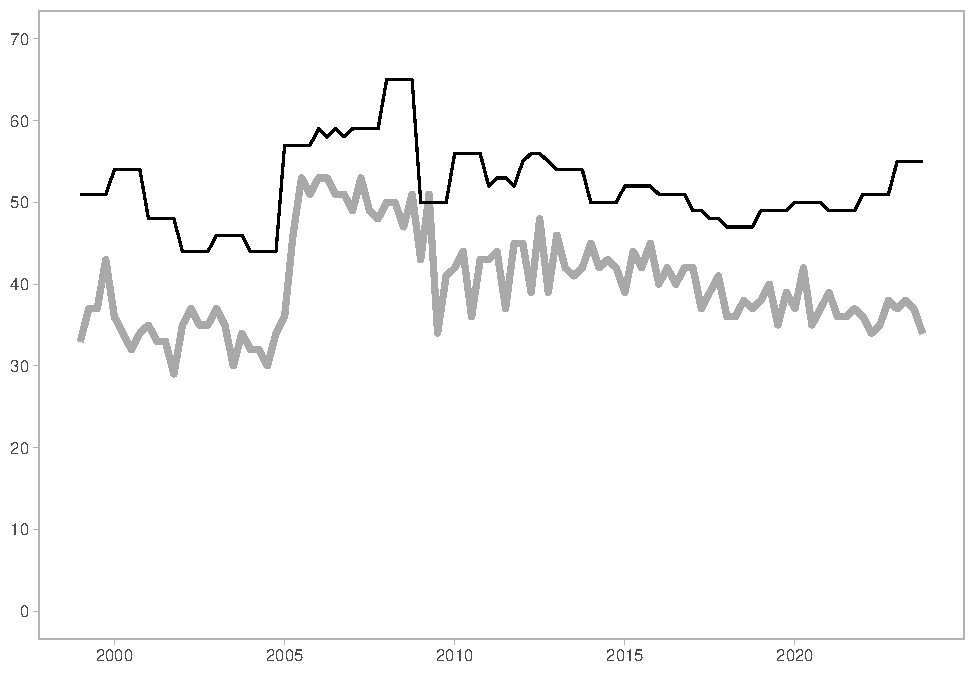
\includegraphics{figures/num_forecasters_over_time.pdf}\\
    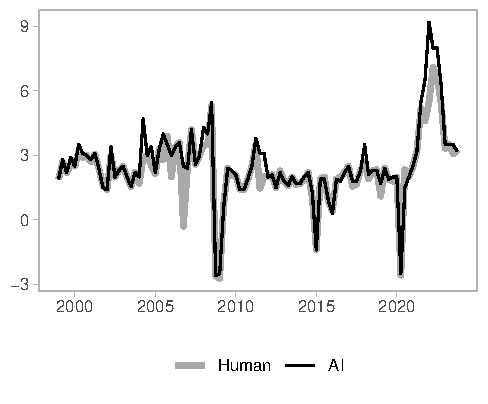
\includegraphics[trim={0 0 0 5.5cm},clip]{figures/human_ai_lgd.pdf}
    \caption{\textbf{Number of forecasters in the SPF panel over time}
    \vspace{5pt}\\
    {\footnotesize The figure shows the number of human and AI forecasters in the SPF panel over time. The number of human forecasters is averaged across variables and forecasting horizons.}
    \vspace{5pt}
    }
    \label{fig:number_forecasters_over_time}
\end{figure}
\clearpage

\begin{figure}[h!]
    \centering
    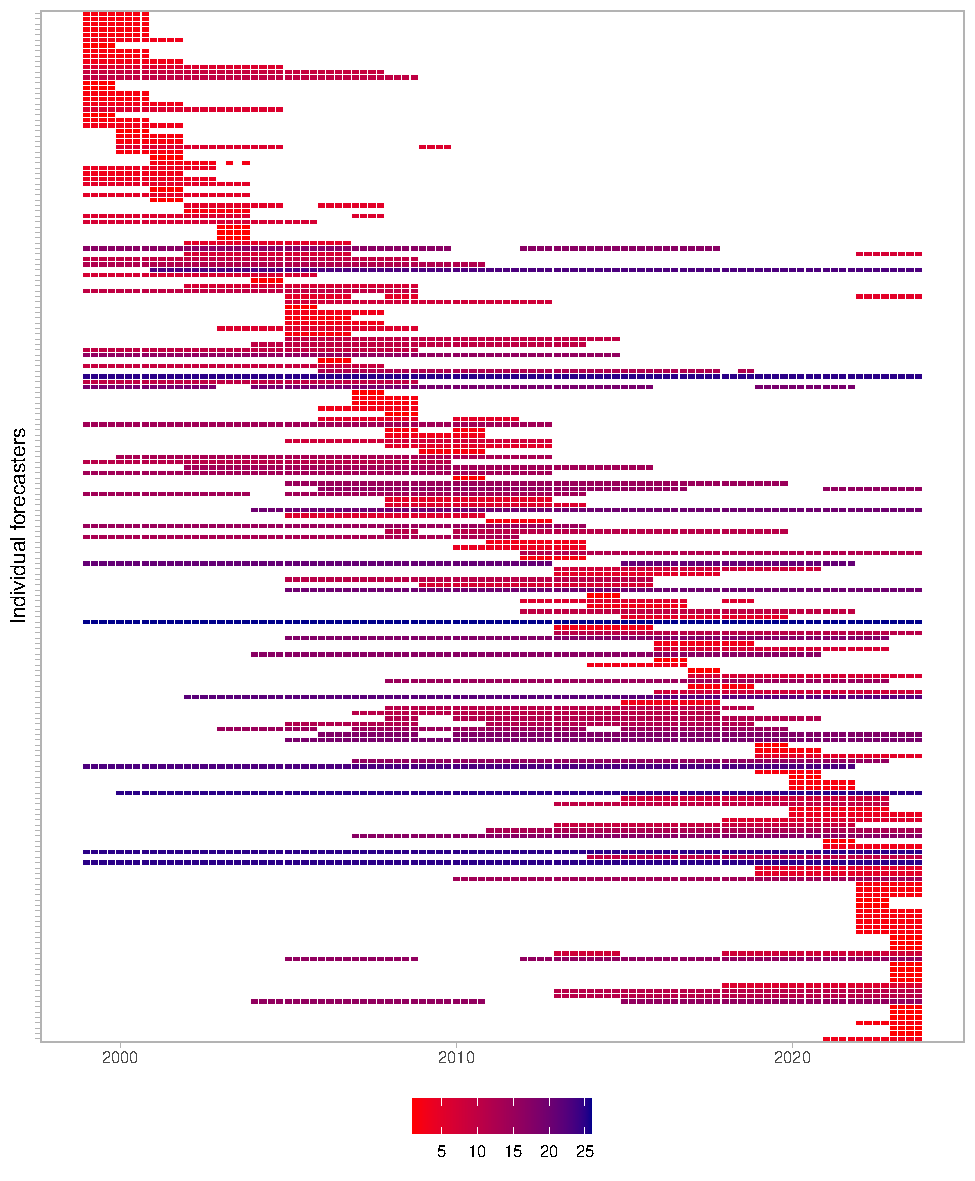
\includegraphics{figures/participation_over_time.pdf}
    \caption{\textbf{Duration of participation of each forecaster individual forecaster in the SPF panel over time}
    \vspace{5pt}\\
    {\footnotesize The figure tracks the duration of individual forecasters' participation in the SPF panel, ranging from a few years to over 25 years. It shows a mix of long-term participants and those with much  shorter tenures.}
    \vspace{5pt}
    }
    \label{fig:participation_over_time}
\end{figure}
\clearpage

\section{Out of Sample Results}\label{app:outofsample}

Tables \ref{tab:MAEs_forecastaccuracy_oos} and \ref{tab:MAEs_forecastaccuracy_oos_best} report MAEs for median and best forecasts, respectively, for the nowcasts and one- and two-quarter-ahead forecasts. At the time of writing, we cannot evaluate the performance of four-quarter forecasts due to lack of realized data values. The results are mixed: the median human forecasts often outperform AI, but the AI survey has generally lower forecasting errors when considering only the best AI and human forecasters. Overall, AI forecasters continue to perform well. We note that these conclusions are based on just a few quarters of observations, and it is therefore difficult to establish statistical significance due to lack of power. 

\begin{table}[h!]
    \centering
    \scriptsize{
    \input{tables/forecast_accuracy_oos.txt}
    }
    \caption{
    \textbf{Out-of-sample forecast accuracy (mean absolute errors) of SPF and AI-generated SPF forecasts}
    \vspace{10pt}\\
    %\footnotesize{Forecast accuracy (mean absolute errors) of SPF and AI-generated SPF forecasts}
    \vspace{10pt}\\
    \footnotesize{The table shows forecast accuracy for the out-of-sample period, 2024 Q1 - 2024 Q4. Forecast accuracy is reported as mean absolute errors (MAEs) of SPF and AI-generated SPF forecasts for various economic indicators across different forecast horizons. For each forecasting horizon, the table boldfaces the lowest MAE value between the AI and human surveys. The P-val column reports p-values and significance levels for randomized tests of the statistical significance of the difference between AI and human MAEs. The tests are based on 10,000 random draws. Significance levels: $^{\star}$ p-value$\leq$0.10, $^{\star\star}$ p-value$\leq$0.05, $^{\star\star\star}$ p-value$\leq$0.01.
}}
    \label{tab:MAEs_forecastaccuracy_oos}
\end{table}
\clearpage

\begin{table}[h!]
    \centering
    \footnotesize{
    \input{tables/forecast_accuracy_best_forecasters_oos.txt}
    }
    \caption{
    \textbf{Out-of-sample forecast accuracy (mean absolute errors) of best human and AI SPF forecasters}
    \vspace{10pt}\\
    \footnotesize{The table shows forecast accuracy for the out-of-sample period, 2024 Q1 - 2024 Q4. Forecast accuracy is reported as mean absolute errors (MAEs) of the best SPF and AI-generated SPF forecasts for various economic indicators across different forecast horizons. The best forecast is the forecast with lowest absolute error for each variable, horizon, and quarter For each forecasting horizon, the table boldfaces the lowest MAE value between the AI and human surveys. The P-val column reports p-values and significance levels for randomized tests of the statistical significance of the difference between AI and human MAEs. The tests are based on 10,000 random draws. Significance levels: $^{\star}$ p-value$\leq$0.10, $^{\star\star}$ p-value$\leq$0.05, $^{\star\star\star}$ p-value$\leq$0.01.
}}
    \label{tab:MAEs_forecastaccuracy_oos_best}
\end{table}

\clearpage
% ============================================================================
% APPENDIX: REASONING MEASURE DEFINITIONS
%============================================================================
% SECTION 6: LEARNING FROM REASONING TEXT -- moved from main text
% ============================================================================


\begin{comment}
\section{Reasoning}
\label{sec:reasoning}

A key advantage of LLM-based forecasting is that researchers can systematically request and examine the reasoning underlying each forecast, which is rarely feasible with traditional surveys. While the Survey of Professional Forecasters (SPF) typically records only point forecasts, we ask the simulated LLM forecasters to provide a short explanatory text for every prediction. We use these texts to recover the \textit{forecasting framework}, i.e., the dominant reasoning approach used to justify the forecast.
\end{comment}

% --------------------------------------------------------------------------
\begin{comment}
 \subsection{Uncertainty}   
\label{sec:reasoning:uncertainty}

We first relate \textit{uncertainty} (linguistic markers that indicate how sure or unsure the forecaster claims to be) to realized accuracy by building a classification that flags forecasters whose language is confident despite poor historical accuracy. Concretely, we compare each forecaster's stated \textit{epistemic stance} (their degree of certainty as conveyed by the text) to their historical errors. For each forecaster, we compute (i) average uncertainty expression from a \textit{multi-dimensional uncertainty score} (a text-based index that aggregates multiple uncertainty- and confidence-related language dimensions; formal construction in Appendix \ref{app:reasoning_measures}) and (ii) mean absolute forecast error, \textit{MAE} (the average absolute difference between the forecast and the realized CPI outcome, in percentage points). We then form four groups using median splits. \textit{Well-calibrated confident} forecasters (low expressed uncertainty, low MAE) state high confidence and are accurate. \textit{Appropriately uncertain} forecasters (high expressed uncertainty, high MAE) acknowledge difficulty and are inaccurate. \textit{Overconfident} forecasters (low expressed uncertainty, high MAE) express confidence despite large errors. The remaining observations form a residual group.

Overconfident forecasters (26\% of the sample) have mean absolute CPI errors of 1.66 pp, while well-calibrated confident forecasters (13\%) have errors of 0.002 pp (effectively perfect). The accuracy gap is large and highly significant ($t = 32.24$, $p < 0.0001$; Table \ref{tab:overconfidence}). Appropriately uncertain forecasters have errors of 1.73 pp, similar to overconfident forecasters, suggesting that acknowledging uncertainty does not by itself improve accuracy, but miscalibrated confidence is particularly harmful.

This relationship is robust to multiple specifications. Regressing errors on a \textit{net uncertainty} measure (defined as uncertainty markers minus confidence markers, so that negative values indicate net confidence; Appendix \ref{app:uncertainty_measures}) yields a marginally significant negative coefficient ($\beta = -0.026$, $p = 0.044$): more balanced epistemic language modestly improves performance, but the magnitude is small relative to the overconfidence effect. The overconfidence classification remains highly predictive after controlling for crisis periods, experience proxies, reasoning sophistication, and other potential confounds.

Crisis periods are especially informative. Uncertainty expression rises by 42\% during crises ($t = 9.29$, $p < 0.0001$), yet overconfidence remains common (and its penalty intensifies), implying that miscalibration is most damaging precisely when uncertainty is genuine.

Finally, the texts display a strong systematic imbalance toward confident phrasing: 77\% of reasoning instances express some to very high confidence and only 3\% express uncertainty; correspondingly, \textit{confidence markers} (e.g., ``will,'' ``certainly,'' ``clearly'') appear in 76\% of forecasts versus \textit{uncertainty markers} (e.g., ``may,'' ``uncertain,'' ``unclear'') in 20\%. This asymmetry may reflect training on authoritative prose that favors confident phrasing. Operationally, overconfidence can be detected using reasoning text plus historical accuracy and it is among the strongest individual-level predictors we identify.

% ----------------------------------------------------------------------------
\subsection{Risk Balance and Consensus}
\label{sec:reasoning:balance}

We next study how \textit{reasoning similarity} (how similar two forecasters' written justifications are) relates to forecast agreement, and whether disagreement patterns reflect stable forecaster characteristics.

For each forecaster pair $(i,j)$ in each quarter $t$, we measure disagreement as the absolute difference in CPI forecasts, $|F_{i,t}-F_{j,t}|$. We measure reasoning similarity using three standard text-similarity components: (i) \textit{TF-IDF cosine similarity} (cosine similarity between term frequency--inverse document frequency vectors, which capture word usage patterns while down-weighting common terms), (ii) \textit{Jaccard overlap} (intersection over union of the two texts' vocabularies, capturing shared words), and (iii) \textit{length similarity} (similarity in word count, capturing similarity in level of detail). We average these components into a \textit{composite similarity score} (Appendix \ref{app:similarity_measures}). Across 151,250 pairwise comparisons over 100 quarters, reasoning similarity is statistically related to forecast agreement but substantively weak: the correlation is small ($r=-0.020$; Table \ref{tab:reasoning_summary}, Panel B) and explains only 0.04\% of the variance in forecast disagreement. This partial decoupling implies that similar numerical forecasts can be reached via different reasoning paths, and similar reasoning does not guarantee similar forecasts.

Splitting pairs by the median of disagreement and the median of composite similarity yields four roughly equal-sized categories. Two behave as expected: high disagreement/low similarity and low disagreement/high similarity. The remaining two are both anomalous and informative. \textit{Puzzling pairs} show high disagreement despite high similarity (24.8\%): the narratives look similar, but the numbers diverge. \textit{Robust consensus pairs} show low disagreement despite low similarity (24.8\%): different narratives or frameworks converge on similar numbers.

These patterns are not random. \textit{Chi-square tests} (tests of whether category assignments are homogeneous across forecasters) reject homogeneous assignment across forecasters ($\chi^2=6084$, $p<0.0001$; Table \ref{tab:reasoning_summary}, Panel B), with forecaster-level variance in category shares 20--30$\times$ larger than under random assignment. We summarize each forecaster's stable propensity with \textit{tendency proportions} (the share of that forecaster's pairwise comparisons falling into each category). \textit{Robust-consensus tendency} (the share of a forecaster's pairs classified as robust consensus) is strongly linked to accuracy: it is negatively correlated with MAE ($r=-0.298$, $p<0.001$), implying about 20\% lower errors. \textit{Puzzling tendency} (the share classified as puzzling) has at most a weak positive association with errors ($r=0.136$, $p=0.059$).

To understand what drives the difference between puzzling and robust-consensus forecasters, we compare the content of their reasoning. Puzzling forecasters mention crisis scenarios 72\% less often ($p<0.0001$), recession risks 45\% less often ($p=0.001$), and housing indicators 39\% less often ($p<0.0001$); they also use 27\% fewer negative or downside-oriented words (Table~\ref{tab:reasoning_summary}, Panel~C). In contrast, they do not differ meaningfully from robust forecasters in non-risk features like response length ($p=0.55$). These results suggest that it is the treatment of risk that best explains the difference. Superficially similar narratives can lead to divergent forecasts when risks are neglected, while multiple reasoning paths can still produce accurate predictions if tail risks are considered.
\end{comment}
% ----------------------------------------------------------------------------
%\subsection{Reasoning Patterns and Consistency}
%\label{sec:reasoning:patterns}

%Beyond uncertainty and risk balance, the dominant reasoning framework used in the text to justify the forecast predicts accuracy.
\section{Reasoning Classification Details}\label{app:reasoning}

\subsection{Keyword Lists}

Each LLM-generated reasoning response is classified using keyword-frequency rules. A response is tagged with a category if it contains at least one keyword from that category's list:

\begin{itemize}
    \item \textbf{Mechanical:} ``trend,'' ``historical,'' ``average,'' ``mean reversion,'' ``pattern,'' ``previous,'' ``past,'' ``typical,'' ``normal,'' ``baseline,'' ``extrapolat.''
    
    \item \textbf{Policy:} ``fed,'' ``federal reserve,'' ``monetary policy,'' ``fiscal,'' ``stimulus,'' ``rate hike,'' ``rate cut,'' ``tightening,'' ``easing,'' ``central bank,'' ``government,'' ``policy response,'' ``intervention.''
    
    \item \textbf{Model:} ``phillips curve,'' ``okun,'' ``gdp growth,'' ``economic model,'' ``structural,'' ``relationship between,'' ``economic theory,'' ``multiplier,'' ``elasticity,'' ``economic indicator,'' ``leading indicator.''
    
    \item \textbf{Event-driven:} ``covid,'' ``pandemic,'' ``crisis,'' ``recession,'' ``shock,'' ``war,'' ``collapse,'' ``lockdown,'' ``unprecedented,'' ``disruption,'' ``financial crisis,'' ``lehman,'' ``subprime,'' ``outbreak,'' ``emergency.''
\end{itemize}

\subsection{ECB-Style Aggregation}

Following the ECB Survey of Professional Forecasters framework:
\begin{align*}
\text{Model-based} &= \text{Model} \cup \text{Mechanical} \\
\text{Judgment-based} &= \text{Policy} \cup \text{Event}
\end{align*}

\subsection{Crisis Period Definitions}

\begin{itemize}
    \item Financial Crisis: 2008 Q3 -- 2009 Q4
    \item COVID-19 Pandemic: 2020 Q1 -- 2020 Q4
    \item Inflation Shock: 2022 Q1 -- 2022 Q4
\end{itemize}
All other quarters are classified as ``Normal'' periods.
\begin{comment}
Performance differences are large (Table \ref{tab:reasoning_summary}, Panel A). Mechanical reasoning yields MAE of 0.765 pp; policy reasoning 0.841 pp; theoretical reasoning 1.156 pp; and event-driven reasoning 1.401 pp. The gap between mechanical and event-driven reasoning is an 83\% increase in error ($p<0.0001$), and it persists after controlling for crisis periods, reasoning length, and information-source mentions.

Event-driven reasoning is especially costly during crises, when it becomes much more prevalent (38\% during crises versus 17\% otherwise). By contrast, mechanical reasoning is equally prevalent in crisis and non-crisis periods and outperforms in both. The evidence points to consistency as the mechanism: mechanical reasoning anchors forecasts in stable regularities, whereas event-driven reasoning reacts to salient developments, consistent with availability bias and recency bias. Taken together, text-based measures of uncertainty calibration, downside-risk coverage, and framework consistency explain substantial cross-sectional variation in forecast accuracy.


%%%%%%%%%%%%%%%%%%%%%%%%%%%%%%%%%%%%%%%%%%%%%%%%%%%%%%%%%%%%%%%%%%
\clearpage
\begin{table}[!htbp]
\centering
\caption{Forecast Accuracy by Epistemic Confidence}
\label{tab:overconfidence}
\begin{tabular}{lcccc}
\toprule
& \multicolumn{2}{c}{\textbf{Low Forecast Error}} & \multicolumn{2}{c}{\textbf{High Forecast Error}} \\
\cmidrule(lr){2-3} \cmidrule(lr){4-5}
& N (\%) & MAE (pp) & N (\%) & MAE (pp) \\
\midrule
\textbf{Low Uncertainty Expression} & & & & \\
\quad Well-Calibrated \& Confident & 839 (13.0\%) & 0.002 & & \\
\quad Overconfident & & & 1,688 (26.1\%) & 1.659 \\
\addlinespace[0.5em]
\textbf{High Uncertainty Expression} & & & & \\
\quad Other & 1,241 (19.2\%) & 0.052 & & \\
\quad Appropriately Uncertain & & & 1,536 (23.8\%) & 1.733 \\
\midrule
\multicolumn{5}{l}{\textit{Key Comparison:}} \\
\quad Overconfident vs Well-Calibrated & \multicolumn{4}{r}{$\Delta$ = 1.657 pp, $t$ = 32.24, $p < 0.0001$} \\
\bottomrule
\end{tabular}
\begin{tablenotes}
\small
\item \textit{Notes:} Classification based on median splits of uncertainty expression (linguistic markers) and absolute CPI forecast error. MAE = Mean Absolute Error in percentage points. N = 6,468 forecaster-quarter observations. Confidence markers (``will,'' ``certainly,'' ``clearly'') appear in 76\% of forecasts; uncertainty markers (``may,'' ``uncertain,'' ``unclear'') appear in 20\%.
\end{tablenotes}
\end{table}

% ============================================================================
% TABLE 2: SUMMARY OF REASONING ANALYSIS FINDINGS
% ============================================================================
% Combines: Risk Balance, Patterns, and Mechanism in one table

\begin{table}[!htbp]
\centering
\caption{Summary of Reasoning Analysis Findings}
\label{tab:reasoning_summary}
\small
\begin{tabular}{llcc}
\toprule
\textbf{Analysis} & \textbf{Finding} & \textbf{Effect} & \textbf{P-value} \\
\midrule
\multicolumn{4}{l}{\textit{Panel A: Reasoning Patterns and Accuracy}} \\
\addlinespace[0.3em]
& Mechanical reasoning (MAE) & 0.765 pp & \\
& Policy reasoning (MAE) & 0.841 pp & \\
& Theoretical reasoning (MAE) & 1.156 pp & \\
& Event-driven reasoning (MAE) & 1.401 pp & \\
& \textit{Mechanical vs Event-driven} & \textit{+83\%} & $<$0.0001 \\
\addlinespace[0.8em]
\midrule
\multicolumn{4}{l}{\textit{Panel B: Forecast Agreement and Reasoning Similarity}} \\
\addlinespace[0.3em]
& Pairwise comparisons (N) & 151,250 & \\
& Disagreement-similarity correlation & $r = -0.020$ & $<$0.0001 \\
& Variance explained & 0.04\% & \\
\addlinespace[0.5em]
& ``Puzzling'' pairs (high disagree, high similar) & 24.8\% & \\
& ``Robust consensus'' pairs (low disagree, low similar) & 24.8\% & \\
\addlinespace[0.5em]
& Forecaster heterogeneity ($\chi^2$) & 6,084 & $<$0.0001 \\
& Corr(Robust tendency, lower errors) & $r = -0.298$ & $<$0.001 \\
\addlinespace[0.8em]
\midrule
\multicolumn{4}{l}{\textit{Panel C: Mechanism: Puzzling vs Robust Forecasters}} \\
\addlinespace[0.3em]
& Crisis mentions (Puzzling vs Robust) & $-$72\% & $<$0.0001 \\
& Recession mentions & $-$45\% & 0.001 \\
& Housing mentions & $-$39\% & $<$0.0001 \\
& Negative tone & $-$27\% & 0.007 \\
\addlinespace[0.3em]
& Reasoning length & n.s. & 0.55 \\
%& Sophistication score & n.s. & 0.44 \\
\bottomrule
\end{tabular}
\begin{tablenotes}
\small
\item \textit{Notes:} Panel A: MAE = Mean Absolute CPI Forecast Error in percentage points. Classification based on dominant reasoning framework. Panel B: Similarity measured via TF-IDF cosine, Jaccard overlap, and length similarity. Panel C: Puzzling forecasters (high disagreement despite similar reasoning) neglect downside risks; robust forecasters (consensus despite different reasoning) incorporate tail scenarios. n.s. = not significant.
\end{tablenotes}
\end{table}

% ============================================================================
\clearpage
\section*{Reasoning Measure Definitions}
\label{app:reasoning_measures}

This appendix defines the reasoning variables used in Tables \ref{tab:overconfidence} and \ref{tab:reasoning_summary}, including construction, classification rules, and statistical tests.

% ----------------------------------------------------------------------------
\subsection*{A.1 Uncertainty Expression Measures}
\label{app:uncertainty_measures}

%\paragraph{Multi-Dimensional Uncertainty and Net Uncertainty.}
We quantify epistemic stance along eight linguistic dimensions (counts per forecast):
\begin{enumerate}
    \item \textit{Explicit Uncertainty:} ``uncertain,'' ``unclear,'' ``difficult to predict,'' ``unpredictable,'' ``unknown,'' ``volatile.''
    \item \textit{Hedging Language:} ``may,'' ``might,'' ``could,'' ``possibly,'' ``perhaps,'' ``likely,'' ``probably,'' ``seems,'' ``appears,'' ``suggests,'' ``potential.''
    \item \textit{Confidence Markers:} ``definitely,'' ``certainly,'' ``clearly,'' ``obviously,'' ``undoubtedly,'' ``sure,'' ``confident,'' ``expect,'' ``will,'' ``strongly.''
    \item \textit{Range Expressions:} numerical ranges via regex (e.g., ``between $X$ and $Y$'', ``$X$--$Y$ percent'').
    \item \textit{Conditional Statements:} conditionals via regex (e.g., ``if\ldots then'', ``depending on'').
    \item \textit{Risk Mentions:} ``risk,'' ``downside,'' ``upside,'' ``tail risk.''
    \item \textit{Probability Language:} ``probability,'' ``chance,'' ``likelihood,'' ``odds.''
    \item \textit{Epistemic Modals:} ``believe,'' ``think,'' ``assume,'' ``suppose,'' ``estimate.''
\end{enumerate}
%\paragraph{Uncertainty measures.}
Let $k \in \{1,\dots,8\}$ index the eight epistemic-language dimensions listed above.
Let $\mathcal{K}^{+}=\{1,2,4,5,6,7,8\}$ denote the seven \emph{uncertainty-indicating} dimensions,
and let $k=3$ denote the \emph{confidence-marker} dimension.
Let $d_{itk}$ be the (normalized) count/score for dimension $k$ for forecaster $i$ in period $t$,
with weights $w_k$.

\emph{Uncertainty-only score:}
\begin{equation}
U^{+}_{it} \;=\; \sum_{k \in \mathcal{K}^{+}} w_k \, d_{itk}.
\end{equation}

\emph{Confidence component:}
\begin{equation}
C_{it} \;=\; w_3 \, d_{it3}.
\end{equation}

\emph{Net Uncertainty:}
\begin{equation}
U^{\text{net}}_{it} \;=\; U^{+}_{it} - C_{it}.
\end{equation}

\noindent\textit{Note:} Because $U^{+}_{it}$ excludes the confidence-marker dimension ($k=3$),
$U^{\text{net}}_{it}$ does not subtract a component already included in $U^{+}_{it}$.

%\paragraph{Overconfidence Classification.}
Next, we assign forecasters to a $2\times 2$ matrix using median splits of (i) average uncertainty expression (forecaster-level mean of $\text{Net Uncertainty}_{it}$) and (ii) mean absolute CPI forecast error. ``Overconfident'' forecasters are below-median on uncertainty expression but above-median on forecast error; ``well-calibrated confident'' forecasters fall below both medians.

% ----------------------------------------------------------------------------
\subsection*{A.2 Reasoning Pattern Classification}
\label{app:pattern_measures}

Each forecast is classified into one of four mutually exclusive reasoning patterns using keyword-frequency rules:
\begin{itemize}
    \item \textbf{Mechanical:} historical regularities and trends. Keywords: ``trend,'' ``average,'' ``typically,'' ``historically,'' ``mean-revert,'' ``pattern,'' ``consistent,'' ``stable,'' ``steady.'' (Example: ``Inflation typically mean-reverts to its long-run average.'')
    \item \textbf{Policy:} institutional or policy responses. Keywords: ``Fed,'' ``Federal Reserve,'' ``FOMC,'' ``monetary policy,'' ``interest rate,'' ``fiscal,'' ``stimulus,'' ``Congress,'' ``central bank.'' (Example: ``The Fed will likely raise rates in response to inflation pressures.'')
    \item \textbf{Model:} structural or other models. Keywords: ``Phillips curve,'' ``Okun's law,'' ``multiplier,'' ``equilibrium,'' ``structural,'' ``model,'' and explicit theory references. (Example: ``Phillips curve dynamics suggest inflation will rise as unemployment falls.'')
    \item \textbf{Event-driven:} salient shocks/crises or specific events. Keywords: ``crisis,'' ``shock,'' ``pandemic,'' ``recession,'' ``collapse,'' ``disruption,'' event names (e.g., ``COVID-19,'' ``financial crisis''), and temporal references to recent events. (Example: ``The economy continues to recover from the 2008 financial crisis.'')
\end{itemize}
If multiple patterns appear, we assign the dominant pattern by relative keyword frequency (word share). Forecasts with no dominant pattern are labeled ``unclear'' and excluded from pattern-specific analyses.

% ----------------------------------------------------------------------------
\subsection*{A.3 Reasoning Similarity Measures}
\label{app:similarity_measures}

For each forecaster pair $(i,j)$ in each quarter $t$, we compute three similarity measures on the reasoning text:
\begin{itemize}
    \item \textbf{TF-IDF Cosine Similarity:} TF-IDF vectors (top 100 informative terms; English stop words removed) and cosine similarity
    \begin{equation}
    \text{Cosine Similarity} = \frac{\mathbf{v}_i \cdot \mathbf{v}_j}{\|\mathbf{v}_i\| \|\mathbf{v}_j\|}.
    \end{equation}
    \item \textbf{Jaccard Similarity:} vocabulary overlap on lowercased tokens
    \begin{equation}
    \text{Jaccard Similarity} = \frac{|W_i \cap W_j|}{|W_i \cup W_j|}.
    \end{equation}
    \item \textbf{Length Similarity:} similarity in word-count detail level
    \begin{equation}
    \text{Length Similarity} = 1 - \frac{|L_i - L_j|}{\max(L_i, L_j)}.
    \end{equation}
\end{itemize}

\paragraph{Composite Similarity Score.}
We aggregate the three measures by arithmetic mean:
\begin{equation}
\text{Composite Similarity} = \frac{1}{3}\left(\text{Cosine} + \text{Jaccard} + \text{Length}\right).
\end{equation}

% ----------------------------------------------------------------------------
\subsection*{A.4 Disagreement-Similarity Classification}
\label{app:disagreement_measures}

%\paragraph{Forecast Disagreement.}
For each pair $(i,j)$ in quarter $t$, disagreement is the absolute difference in CPI forecasts:
\begin{equation}
\text{Disagreement}_{ij,t} = |F_{i,t} - F_{j,t}|.
\end{equation}

%\paragraph{Case Classification.}
\noindent Using median splits of $\text{Disagreement}_{ij,t}$ and Composite Similarity, each pair is assigned to:
\begin{itemize}
    \item \textit{Puzzling:} high disagreement ($>$ median) and high similarity ($>$ median).
    \item \textit{Robust Consensus:} low disagreement ($\leq$ median) and low similarity ($\leq$ median).
    \item \textit{Expected (High-Low):} high disagreement and low similarity.
    \item \textit{Expected (Low-High):} low disagreement and high similarity.
\end{itemize}

%\paragraph{Forecaster Tendency Proportions.}
For each forecaster, we compute the share of their pairwise comparisons in each category. \textit{Robust tendency} is the share classified as Robust Consensus; \textit{Puzzling tendency} is the share classified as Puzzling.

% ----------------------------------------------------------------------------
\subsection*{A.5 Topic Mention Variables}
\label{app:topic_measures}

Topic mentions are identified by keyword matching in reasoning text. Each variable is coded at the forecast level as an indicator (1 if any keyword appears, 0 otherwise), then averaged to forecaster-level proportions.
\begin{itemize}
    \item \textbf{Crisis Mentions:} ``crisis,'' ``crises,'' ``meltdown,'' ``collapse,'' ``turmoil,'' plus specific crisis phrases (e.g., ``financial crisis,'' ``debt crisis'').
    \item \textbf{Recession Mentions:} ``recession,'' ``recessionary,'' ``contraction,'' ``downturn,'' ``negative growth.''
    \item \textbf{Housing Mentions:} ``housing,'' ``home,'' ``mortgage,'' ``real estate,'' ``residential,'' ``housing starts.''
    \item \textbf{Federal Reserve Mentions:} ``Fed,'' ``Federal Reserve,'' ``FOMC,'' ``monetary policy,'' ``interest rate,'' ``rate hike,'' ``rate cut,'' ``central bank.''
\end{itemize}

% ----------------------------------------------------------------------------
\subsection*{A.6 Statistical Tests}
\label{app:stat_tests}

%\paragraph{Forecaster Heterogeneity (Chi-square Test).}

We test whether puzzling/robust category shares differ systematically across forecasters using a chi-square test of independence on the forecaster $\times$ category contingency table. Under the null hypothesis, case-category assignment is independent of forecaster identity; equivalently, each forecaster follows the pooled category distribution. The test statistic is
\begin{equation}
\chi^2 = \sum_{i}\sum_{j} \frac{(O_{ij} - E_{ij})^2}{E_{ij}},
\end{equation}
where $O_{ij}$ is forecaster $i$'s observed count in category $j$ and the expected count under the null is
\begin{equation}
E_{ij}=\frac{O_{i\cdot}\,O_{\cdot j}}{O_{\cdot\cdot}},
\end{equation}
with $O_{i\cdot}=\sum_{j}O_{ij}$, $O_{\cdot j}=\sum_{i}O_{ij}$, and $O_{\cdot\cdot}=\sum_{i}\sum_{j}O_{ij}$.
Because the four categories are defined by median splits, the pooled marginal shares $O_{\cdot j}/O_{\cdot\cdot}$ are approximately (and in the absence of ties, exactly) $25\%$ each. Thus, the expected counts coincide with those from a uniform $25/25/25/25$ benchmark, but this uniformity arises mechanically from the median-split construction rather than being an additional assumption.

%\paragraph{Variance Ratio.}
We compare observed variance in forecaster-level proportions to binomial variance under random assignment. For category share $p$ based on $n$ pairs, the expected variance is $p(1-p)/n$. The variance ratio is the observed variance divided by this benchmark; ratios $\gg 1$ indicate systematic heterogeneity.

\vspace{2em}
\noindent\textit{Implementation:} Text processing is implemented in Python using standard NLP tooling (NLTK tokenization; scikit-learn TF-IDF). Regular expressions follow the Python \texttt{re} syntax. Code is available upon request.

% ---------------------------------------------------------------------------

\clearpage
\section{Robustness Checks}\label{{app:robustness}}

\subsection{Expanded Prompt}\label{sec:appendix_expanded_prompt}

As a robustness check, we employ an alternative approach to creating synthetic forecast personas: an expanded prompt based on forecaster biographies generated using an LLM and personal characteristics. Table \ref{tab:personas_definition_examples} presents examples of personas generated by both methods:

\vspace{1em}
\begin{table}[!htbp]
\centering
\footnotesize
\captionsetup{justification=centering}
\caption{Fictional Example of Main and Expanded Persona Prompts}
\begin{tabular}{p{0.48\textwidth} p{0.04\textwidth} p{0.5\textwidth}}
\hline
\textbf{Main Persona Prompt} && \textbf{Expanded Persona Prompt} \\ \hline
You are a participant on a panel of Survey of Professional Forecasters. Your name is Alexandra Bryson, you graduated from University of New Hampshire with a M.A. in Economics around 2024. Today, you work as a Senior Quantitative Analyst at Ethan Investments, an Asset Management organization based in Boston, Massachusetts. You are originally from the USA. && You are a Senior Quantitative Analyst at Ethan Investments with a Master's degree in Economics. Your expertise lies in macroeconomic forecasting, and you actively participate in the Survey of Professional Forecasters for the Federal Reserve Bank of Philadelphia. Known for your meticulous approach to data analysis, you excel in interpreting complex economic information and translating it into actionable forecasts. Your experience at Ethan Investments has honed your forecasting skills, making you a trusted source of economic predictions in the financial industry. Your dedication to staying informed about the latest economic developments sets you apart as a reliable and knowledgeable forecaster. \\ \hline
\end{tabular}
\label{tab:personas_definition_examples}

    \parbox{16cm}{\small \vspace{0.5em} \textit{Note:} The example uses fictional characteristics for privacy reasons. However, we feed the models all names that were featured on the acknowledgment SPF lists.}

\end{table}

The first approach is used in the main analysis and described in the main body of the paper. The second approach (``Expanded Persona Prompt'') is  involves crafting synthetic personas using biographical narratives. We use OpenAI's Assistant API to interact with a specialized AI assistant designed for this task. Specifically, we employ the following system prompt:

\begin{quote} \textit{You are designed to gather information on the background and biography of a professional forecaster who participates in the Survey of Professional Forecasters for the Federal Reserve Bank of Philadelphia. Your task is to create a persona, with a maximum of 200 words, that accurately represents their most important characteristics, forecasting expertise, background, and overall persona. Do not reference them by name, but mentioning associated organizations is acceptable. Each text should start with ``You are ...". Use simple words and easy-to-read text.} \end{quote}

The assistant processes the biographical information obtained from each forecaster's online profile and generates a synthesized persona as output. This approach captures the essence of the forecaster's expertise and background without revealing their identity, allowing the LLM to produce forecasts that embody the forecaster's professional persona.

\subsection{Comparison Across Models}

We evaluate different AI models and settings to assess their performance in economic forecasting tasks. These models represent combinations of:

\begin{itemize}
    \item LLM Architectures: GPT-3.5, GPT-4, GPT-4o-mini, Llama-3.3-70B-Instruct-Turbo, and DeepSeek-V3.
    \item Temperature Settings: 0 (deterministic) and 1 (stochastic)
    \item Persona Prompts: main and expanded prompts, as discussed in Section \ref{sec:appendix_expanded_prompt}
\end{itemize}

The results support the main conclusions from the paper and are available upon request.
\end{comment}

% ---------------------------------------------------------------------------
\clearpage
\section{Simulating the SPF With an AR(1) Model}\label{app:AR1}

This appendix shows forecast results generated by a simple AR(1) model on median human forecasts. Specifically, letting $\bar h_t$ denote the median human forecast of any variable in the SPF, the AR(1) model takes the following form:
\begin{align}
    \bar h_t = \alpha + \rho \bar h_{t-1}   + \varepsilon_t,
\end{align}
where $\varepsilon_t$ is independent and identically distributed according to a normal distribution with mean zero and a constant variance. The coefficients are estimated using an expanding window, such that predictions for the survey at time $t$ are based on information up until time $t-1$. 

Table \ref{tab:MAEs_AR1} reports mean absolute errors of AI-generated SPF forecasts and forecasts implied by an AR(1) model on median human SPF forecasts, relative to the mean absolute errors of human SPF forecasts. The statistical significance of the difference between AI and AR(1) forecasts is evaluated using the Diebold and Mariano test (\cite{diebold1995comparing}, \cite{diebold1997evaluating}). The results show that human forecasters do not rely solely on AR(1) models for generating SPF forecasts, as the relative mean absolute error of AR(1) forecasts are generally different from one. In addition, the results show that AI forecasts add value beyond the AR(1) model, as the AI and AR(1) model are statistically different and the relative mean absolute error is lower for AI forecasts compared with AR(1) forecasts, almost everywhere. 

\begin{table}[h!]
    \centering
    \scriptsize{
    \input{tables/forecast_accuracy_ar1_relative_comparison.txt}
    }
    \caption{
    \textbf{Forecast accuracy (mean absolute errors) of AI-generated and AR(1) SPF forecasts relative to human accuracy}
    \vspace{10pt}\\
    %\footnotesize{Forecast accuracy (mean absolute errors) of SPF and AI-generated SPF forecasts}
    \vspace{5pt}\\
    \footnotesize{The table shows forecast accuracy reported as mean absolute errors of AI-generated SPF forecasts and forecasts implied by an AR(1) model of human SPF forecasts relative to the mean absolute errors of human SPF forecasts. Accuracy is reported for different forecast horizons, with 0, 1 and 4 denoting nowcast, one quarter and four quarters ahead, respectively. For each forecasting horizon, the table boldfaces the lowest MAE relative value between the AI and AR(1) model. The P-val column reports p-values and significance levels for Diebold and Mariano \citeyear{diebold1997evaluating} tests of the statistical significance of the difference between AI and AR(1) forecasts. Significance levels: $^{\star}$ p-value$\leq$0.10, $^{\star\star}$ p-value$\leq$0.05, $^{\star\star\star}$ p-value$\leq$0.01}}
    \label{tab:MAEs_AR1}
\end{table}
\clearpage

\begin{comment}
\begin{figure}[htpb!]
    \centering
    \subfloat[CPI inflation rate, one quarter ahead]{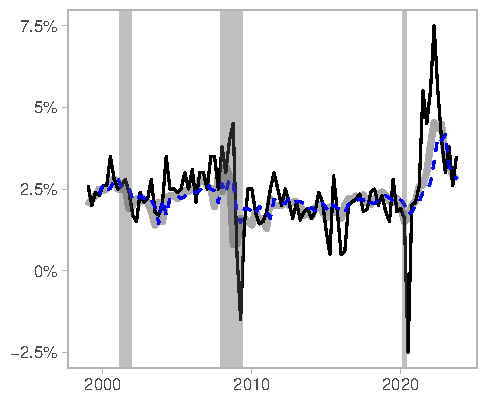
\includegraphics{figures/ts_median_with_ar1_CPI_1.pdf}}
    \subfloat[CPI inflation rate, four quarters ahead]{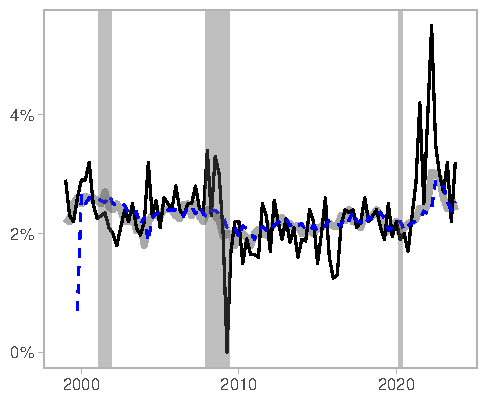
\includegraphics{figures/ts_median_with_ar1_CPI_4.pdf}}\\
    \subfloat[3-month Treasury bill rate, one quarter ahead]{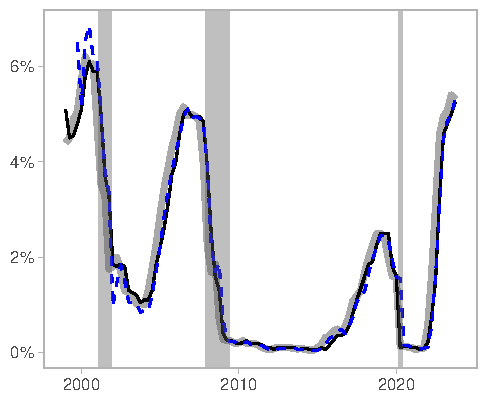
\includegraphics{figures/ts_median_with_ar1_TBILL_1.pdf}}
    \subfloat[3-month Treasury bill rate, four quarters ahead]{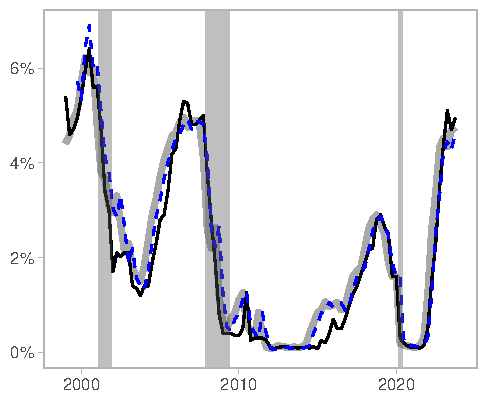
\includegraphics{figures/ts_median_with_ar1_TBILL_4.pdf}}\\
    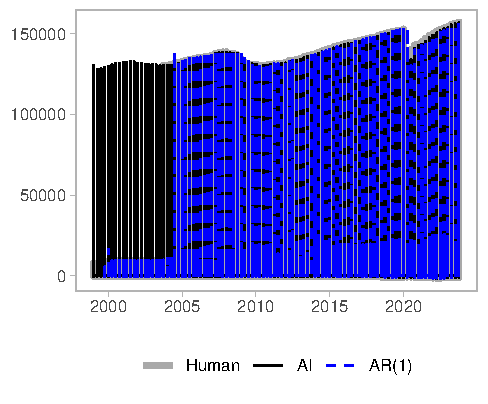
\includegraphics[trim={0 0 0 170pt},clip]{figures/human_ai_ar1_lgd.pdf}
    \\
    \emph{(Figure continues on next page)}
    \caption{\textbf{SPF, AI-generated, and AR(1) median forecasts}
    \vspace{5pt}\\
    {\footnotesize The figure shows the one- and four-quarter ahead median human, AI-generated, and AR(1)-generated SPF forecasts for the (a)-(b) CPI inflation rate, (c)-(d) 3-month Treasury bill rate, (e)-(f) unemployment rate, and (g)-(h) real GDP index. Shaded areas show NBER recession quarters.}
    \vspace{5pt}
    }
    \label{fig:median_forecasts_with_ar1}
\end{figure}
\clearpage
\begin{figure}[h!]\ContinuedFloat
    \centering
    \subfloat[Unemployment rate, one quarter ahead]{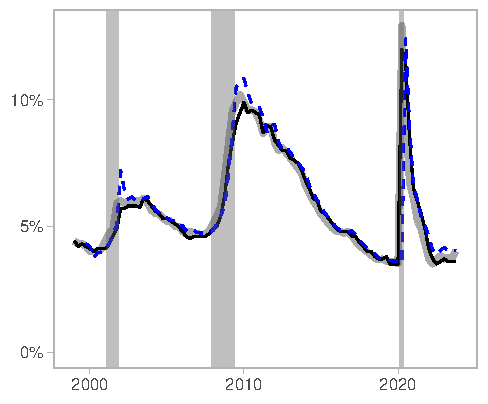
\includegraphics{figures/ts_median_with_ar1_UNEMP_1.pdf}}
    \subfloat[Unemployment rate, four quarters ahead]{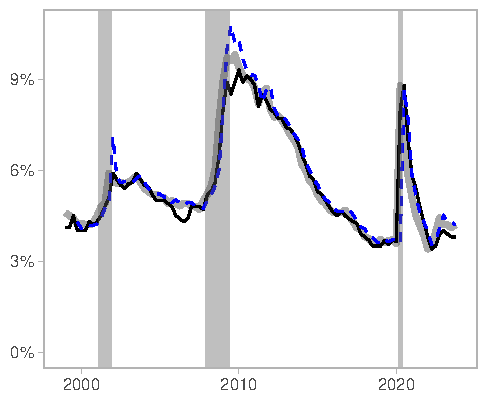
\includegraphics{figures/ts_median_with_ar1_UNEMP_4.pdf}}\\
    \subfloat[Real GDP index, one quarter ahead]{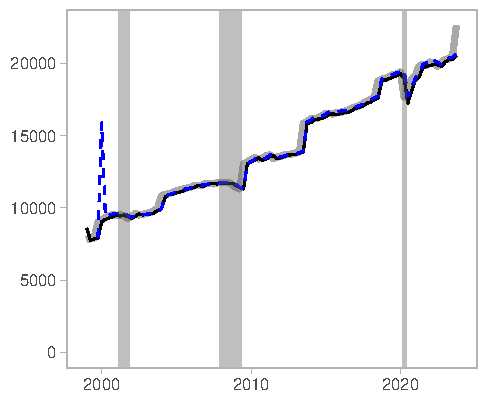
\includegraphics{figures/ts_median_with_ar1_RGDP_1.pdf}}
    \subfloat[Real GDP index, four quarters ahead]{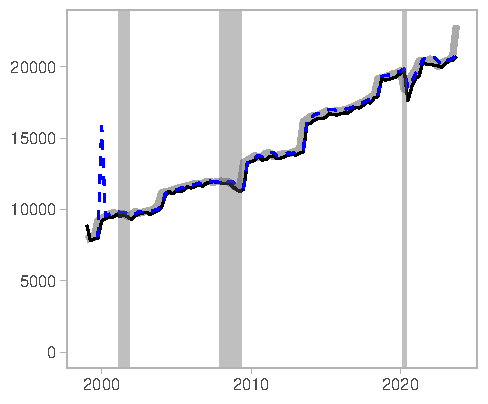
\includegraphics{figures/ts_median_with_ar1_RGDP_4.pdf}}\\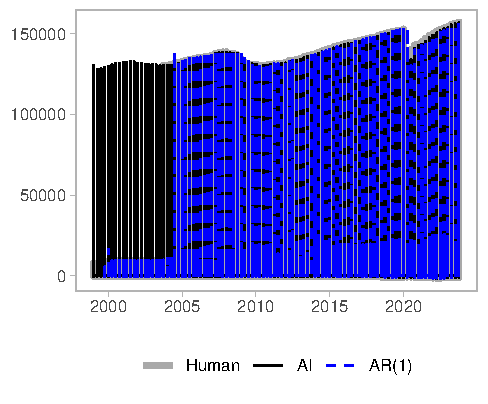
\includegraphics[trim={0 0 0 170pt},clip]{figures/human_ai_ar1_lgd.pdf}
    \caption{\textbf{SPF, AI-generated, and AR(1) median forecasts} \emph{(continued)}
    \vspace{5pt}
    }
    \label{fig:median_forecasts_with_ar1}
\end{figure}
\clearpage
\newpage
\end{comment}

\begin{comment}
\subsection{Out-of-sample results through 2026 Q1}\label{app:outofsample_new}

Tables~\ref{tab:MAE_RMSE_oos_median_h01} and~\ref{tab:MAE_RMSE_oos_best_h01} extend the out-of-sample validation exercise through 2026 Q1. The exercise uses the two model implementations and the four key variables emphasized in the main text: CPI inflation, the 3-month Treasury bill rate, the unemployment rate, and real GDP. We focus on the two short-horizon forecasts that are most relevant for real-time monitoring: the current-quarter nowcast (horizon~0) and the one-quarter-ahead forecast (horizon~1). The comparison is restricted to model-specific post-cutoff survey quarters and to forecast horizons for which a realized target-quarter value is available.

For each horizon $h$, forecasts made in survey quarter $t$ are compared with the realized value in quarter $t+h$. This ensures that nowcasts and one-quarter-ahead forecasts are evaluated against the corresponding target quarter rather than against the value available at the survey date.

Table~\ref{tab:MAE_RMSE_oos_median_h01} reports MAEs and RMSEs for the AI-generated median and the SPF median. Table~\ref{tab:MAE_RMSE_oos_best_h01} reports the corresponding best-forecaster comparison. In the latter table, the best human forecaster is selected ex post within each variable--horizon--survey-quarter cell as the individual SPF response with the lowest absolute error; the best AI forecaster is selected analogously within the synthetic panel. The best-forecaster exercise is therefore an upper-bound comparison rather than an implementable forecasting rule.

The results remain mixed across variables, horizons, and model implementations. The AI-generated medians often track the SPF medians closely, but the SPF median has lower errors in many cells, while the AI median remains competitive in selected short-horizon comparisons. The ex-post best-forecaster comparison is a demanding upper-bound benchmark: selecting the closest individual human response in each cell often yields very small errors. These results should be interpreted cautiously because the post-cutoff sample is short, especially for the Claude Haiku implementation, whose out-of-sample window begins later and therefore yields fewer paired survey quarters.

\begin{table}[h!]
\centering
\scriptsize
\caption{
\textbf{Out-of-sample forecast accuracy (MAE and RMSE) of SPF and AI-generated SPF median forecasts (nowcast and one quarter ahead)}
\vspace{10pt}\\
\footnotesize{The table reports out-of-sample forecast accuracy for model-specific post-cutoff survey quarters. Forecast accuracy is reported as mean absolute errors (MAEs) and root mean squared errors (RMSEs) of AI-generated and SPF median forecasts. For horizon $h$, forecasts made in survey quarter $t$ are evaluated against realizations in target quarter $t+h$. For each horizon, the table boldfaces the lower MAE and RMSE values between the AI and human SPF median. The P-val column reports paired randomized p-values for MAE differences based on 10,000 random sign draws. $N$ is the number of paired survey quarters. Significance: $^{\star}p<0.10$, $^{\star\star}p<0.05$, $^{\star\star\star}p<0.01$.}
}
\label{tab:MAE_RMSE_oos_median_h01}
\resizebox{\textwidth}{!}{%
\begin{tabular}{lcccccccccccc}
\toprule
\textbf{Horizon (quarters)} & \multicolumn{6}{c}{\textbf{0}} & \multicolumn{6}{c}{\textbf{1}} \\
\cmidrule(lr){2-7} \cmidrule(lr){8-13}
 & AI MAE & Human MAE & AI RMSE & Human RMSE & P-val & N & AI MAE & Human MAE & AI RMSE & Human RMSE & P-val & N \\
\midrule
\multicolumn{13}{l}{\textit{Panel A: GPT-4o-mini}} \\
\addlinespace[2pt]
CPI Inflation Rate & 1.27 & \textbf{0.83} & 1.37 & \textbf{0.92} & 0.03$^{\star\star}$ & 9 & \textbf{0.90} & 0.90 & 1.16 & \textbf{1.01} & 1.00 & 8 \\
Treasury Bill Rate (3M) & 0.18 & \textbf{0.09} & 0.26 & \textbf{0.10} & 0.16 & 9 & 0.24 & \textbf{0.11} & 0.36 & \textbf{0.15} & 0.22 & 8 \\
Unemployment Rate & 0.11 & \textbf{0.06} & 0.13 & \textbf{0.09} & 0.23 & 9 & 0.19 & \textbf{0.12} & 0.21 & \textbf{0.14} & 0.17 & 8 \\
Real GDP & 181 & \textbf{116} & 217 & \textbf{154} & 0.06$^{\star}$ & 9 & 273 & \textbf{218} & 320 & \textbf{252} & 0.13 & 8 \\
\midrule
\multicolumn{13}{l}{\textit{Panel B: Claude Haiku 3.5}} \\
\addlinespace[2pt]
CPI Inflation Rate & 1.07 & \textbf{0.84} & 1.23 & \textbf{0.95} & 0.03$^{\star\star}$ & 6 & \textbf{0.80} & 0.86 & \textbf{0.93} & 0.95 & 0.63 & 5 \\
Treasury Bill Rate (3M) & 0.26 & \textbf{0.09} & 0.33 & \textbf{0.10} & 0.03$^{\star\star}$ & 6 & 0.34 & \textbf{0.12} & 0.40 & \textbf{0.18} & 0.06$^{\star}$ & 5 \\
Unemployment Rate & 0.10 & \textbf{0.04} & 0.11 & \textbf{0.06} & 0.06$^{\star}$ & 6 & 0.10 & \textbf{0.10} & 0.12 & \textbf{0.11} & 0.81 & 5 \\
Real GDP & 188 & \textbf{148} & 236 & \textbf{183} & 0.38 & 6 & 279 & \textbf{232} & 323 & \textbf{259} & 0.44 & 5 \\
\bottomrule
\end{tabular}%
}
\end{table}

\clearpage

\begin{table}[h!]
\centering
\scriptsize
\caption{
\textbf{Out-of-sample forecast accuracy (MAE and RMSE) of best human and AI SPF forecasters (nowcast and one quarter ahead)}
\vspace{10pt}\\
\footnotesize{The table reports out-of-sample forecast accuracy for model-specific post-cutoff survey quarters. Forecast accuracy is reported as mean absolute errors (MAEs) and root mean squared errors (RMSEs) of the best AI-generated and best human SPF forecasts. The best forecast is selected ex post as the individual forecast with the lowest absolute error within each variable--horizon--survey-quarter--panel cell. For horizon $h$, forecasts made in survey quarter $t$ are evaluated against realizations in target quarter $t+h$. For each horizon, the table boldfaces the lower MAE and RMSE values between the AI and human SPF panels. The P-val column reports paired randomized p-values for MAE differences based on 10,000 random sign draws. $N$ is the number of paired survey quarters. Significance: $^{\star}p<0.10$, $^{\star\star}p<0.05$, $^{\star\star\star}p<0.01$.}
}
\label{tab:MAE_RMSE_oos_best_h01}
\resizebox{\textwidth}{!}{%
\begin{tabular}{lcccccccccccc}
\toprule
\textbf{Horizon (quarters)} & \multicolumn{6}{c}{\textbf{0}} & \multicolumn{6}{c}{\textbf{1}} \\
\cmidrule(lr){2-7} \cmidrule(lr){8-13}
 & AI MAE & Human MAE & AI RMSE & Human RMSE & P-val & N & AI MAE & Human MAE & AI RMSE & Human RMSE & P-val & N \\
\midrule
\multicolumn{13}{l}{\textit{Panel A: GPT-4o-mini}} \\
\addlinespace[2pt]
CPI Inflation Rate & 0.93 & \textbf{0.07} & 1.11 & \textbf{0.14} & 0.01$^{\star\star}$ & 9 & 0.57 & \textbf{0.18} & 0.82 & \textbf{0.25} & 0.03$^{\star\star}$ & 8 \\
Treasury Bill Rate (3M) & 0.15 & \textbf{0.00} & 0.21 & \textbf{0.01} & 0.00$^{\star\star\star}$ & 9 & 0.15 & \textbf{0.01} & 0.25 & \textbf{0.02} & 0.13 & 8 \\
Unemployment Rate & 0.10 & \textbf{0.00} & 0.13 & \textbf{0.00} & 0.03$^{\star\star}$ & 9 & 0.11 & \textbf{0.01} & 0.16 & \textbf{0.04} & 0.06$^{\star}$ & 8 \\
Real GDP & 180 & \textbf{45} & 216 & \textbf{80} & 0.01$^{\star\star\star}$ & 9 & 227 & \textbf{93} & 288 & \textbf{137} & 0.03$^{\star\star}$ & 8 \\
\midrule
\multicolumn{13}{l}{\textit{Panel B: Claude Haiku 3.5}} \\
\addlinespace[2pt]
CPI Inflation Rate & 0.81 & \textbf{0.04} & 1.02 & \textbf{0.06} & 0.03$^{\star\star}$ & 6 & 0.54 & \textbf{0.12} & 0.72 & \textbf{0.14} & 0.13 & 5 \\
Treasury Bill Rate (3M) & 0.19 & \textbf{0.00} & 0.24 & \textbf{0.01} & 0.03$^{\star\star}$ & 6 & 0.23 & \textbf{0.01} & 0.30 & \textbf{0.02} & 0.13 & 5 \\
Unemployment Rate & 0.08 & \textbf{0.00} & 0.10 & \textbf{0.00} & 0.06$^{\star}$ & 6 & 0.07 & \textbf{0.00} & 0.09 & \textbf{0.00} & 0.25 & 5 \\
Real GDP & 160 & \textbf{59} & 217 & \textbf{96} & 0.09$^{\star}$ & 6 & 196 & \textbf{84} & 273 & \textbf{113} & 0.25 & 5 \\
\bottomrule
\end{tabular}%
}
\end{table}

\clearpage

\begin{figure}[htpb!]
    \centering
    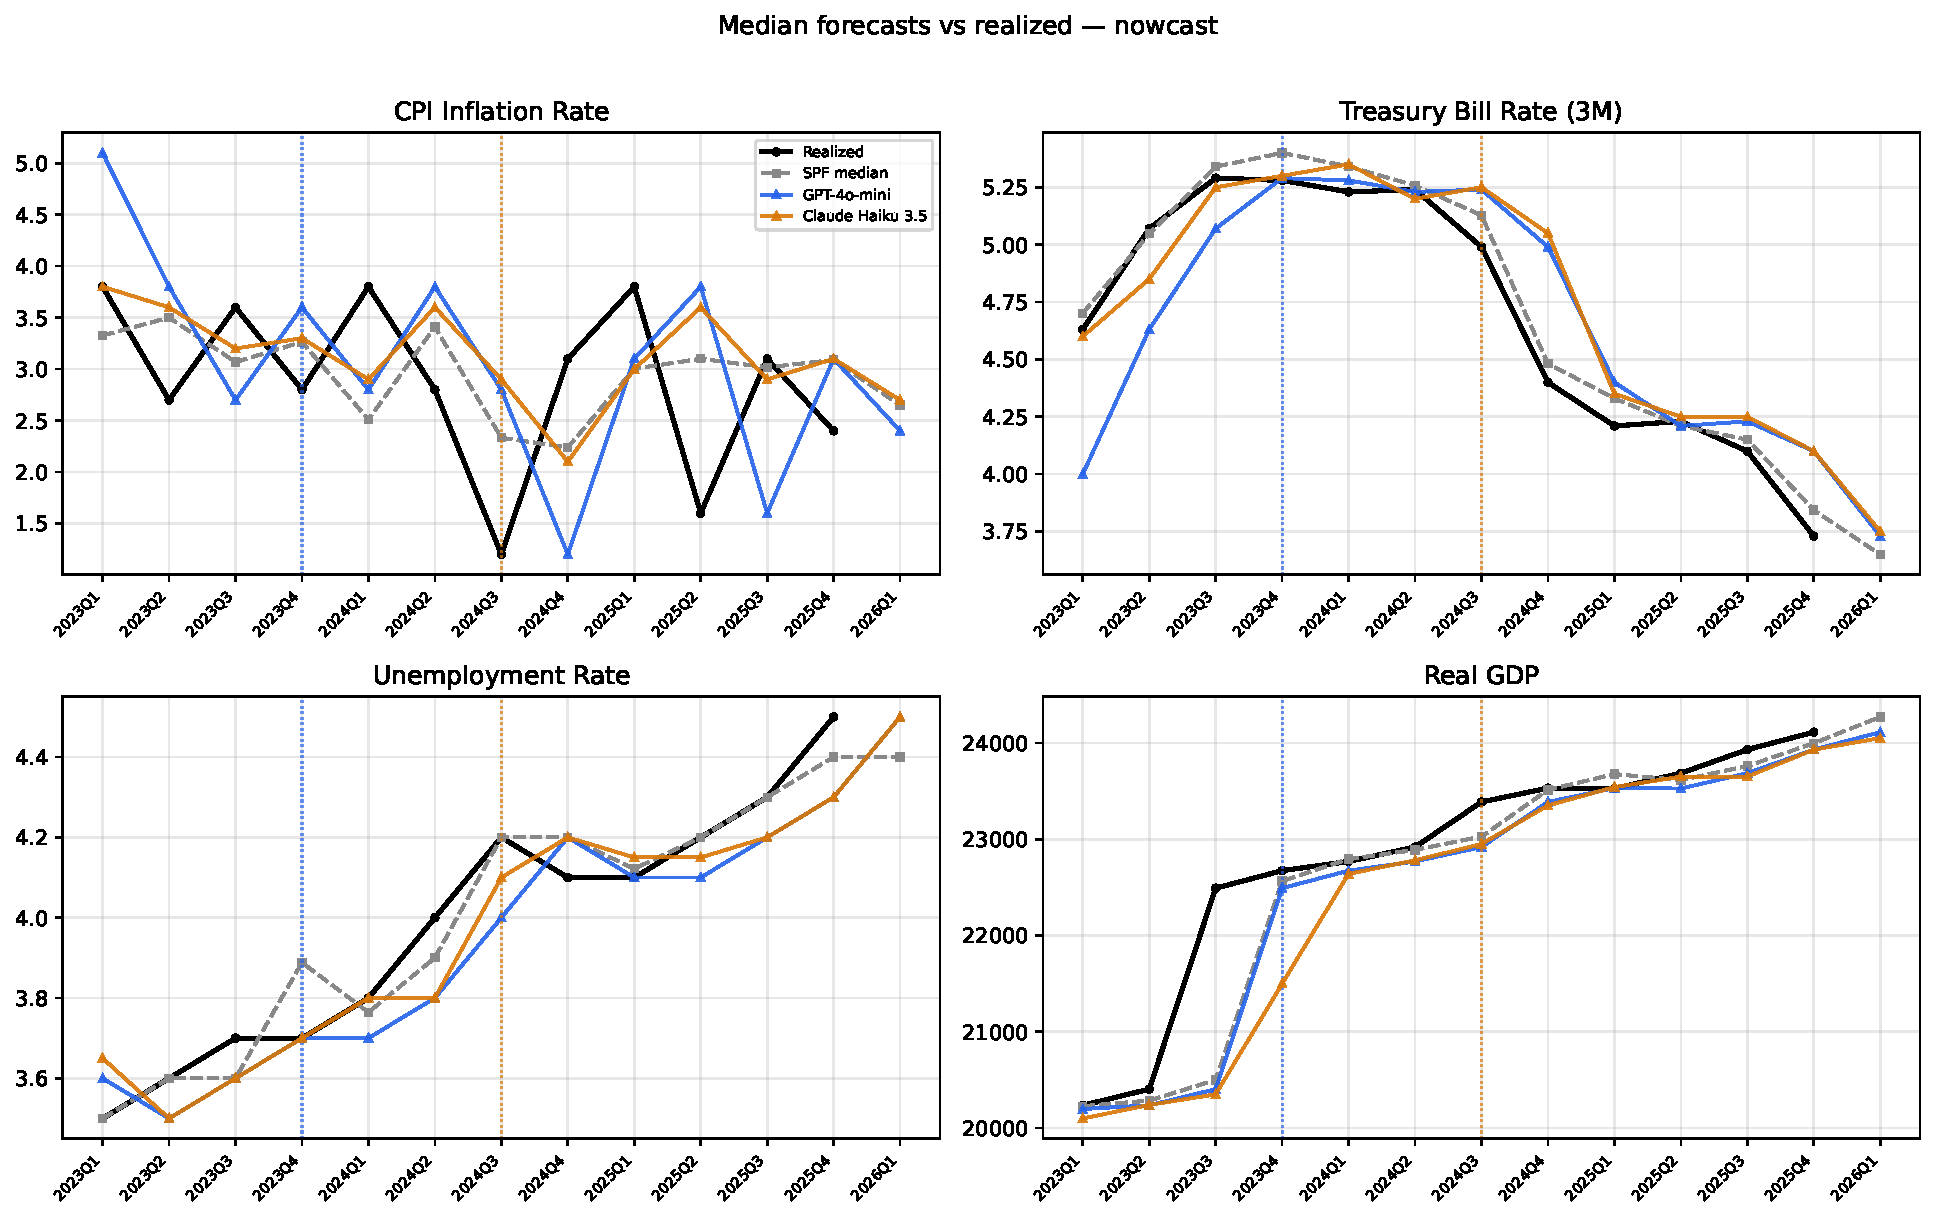
\includegraphics[width=\textwidth]{figures/oosnew/median_forecasts_vs_realized_t.pdf}
    \caption{\textbf{SPF, AI-generated, and realized outcomes: nowcast}
    \vspace{5pt}\\
    {\footnotesize The figure shows nowcast median SPF and AI-generated forecasts, together with realized target-quarter values, for the CPI inflation rate, real GDP index, 3-month Treasury bill rate, and unemployment rate. The black line denotes realized target values; the gray dashed line denotes the SPF median. The vertical dotted lines indicate model-specific out-of-sample starts.}
    \vspace{5pt}}
    \label{fig:oos_levels_t_two_models}
\end{figure}

\clearpage

\begin{figure}[htpb!]
    \centering
    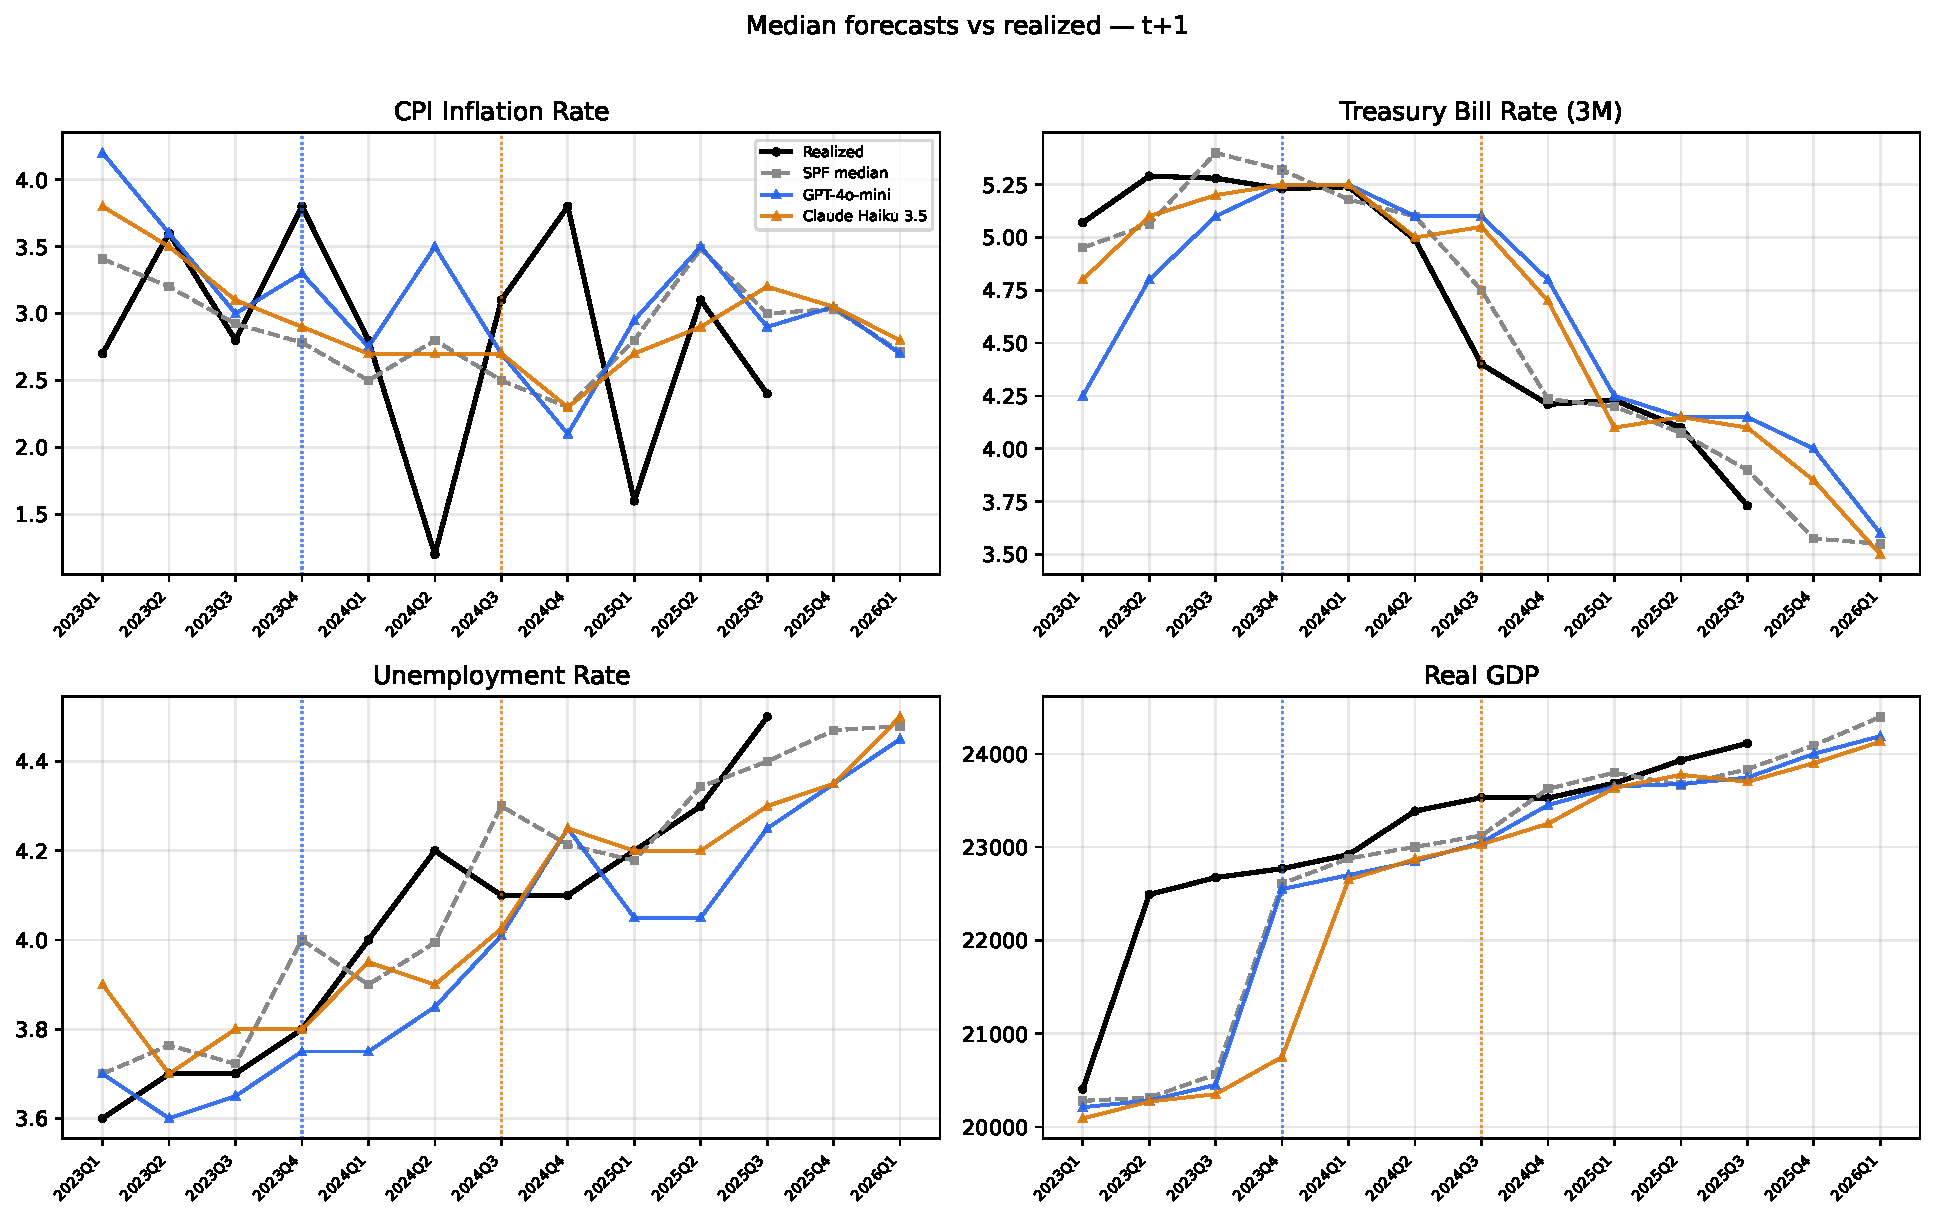
\includegraphics[width=\textwidth]{figures/oosnew/median_forecasts_vs_realized_tp1.pdf}
    \caption{\textbf{SPF, AI-generated, and realized outcomes: one quarter ahead}
    \vspace{5pt}\\
    {\footnotesize The figure shows one-quarter-ahead median SPF and AI-generated forecasts, together with realized target-quarter values, for the CPI inflation rate, real GDP index, 3-month Treasury bill rate, and unemployment rate. The black line denotes realized target values; the gray dashed line denotes the SPF median. The vertical dotted lines indicate model-specific out-of-sample starts.}
    \vspace{5pt}}
    \label{fig:oos_levels_tp1_two_models}
\end{figure}

\clearpage

\begin{figure}[htpb!]
    \centering
    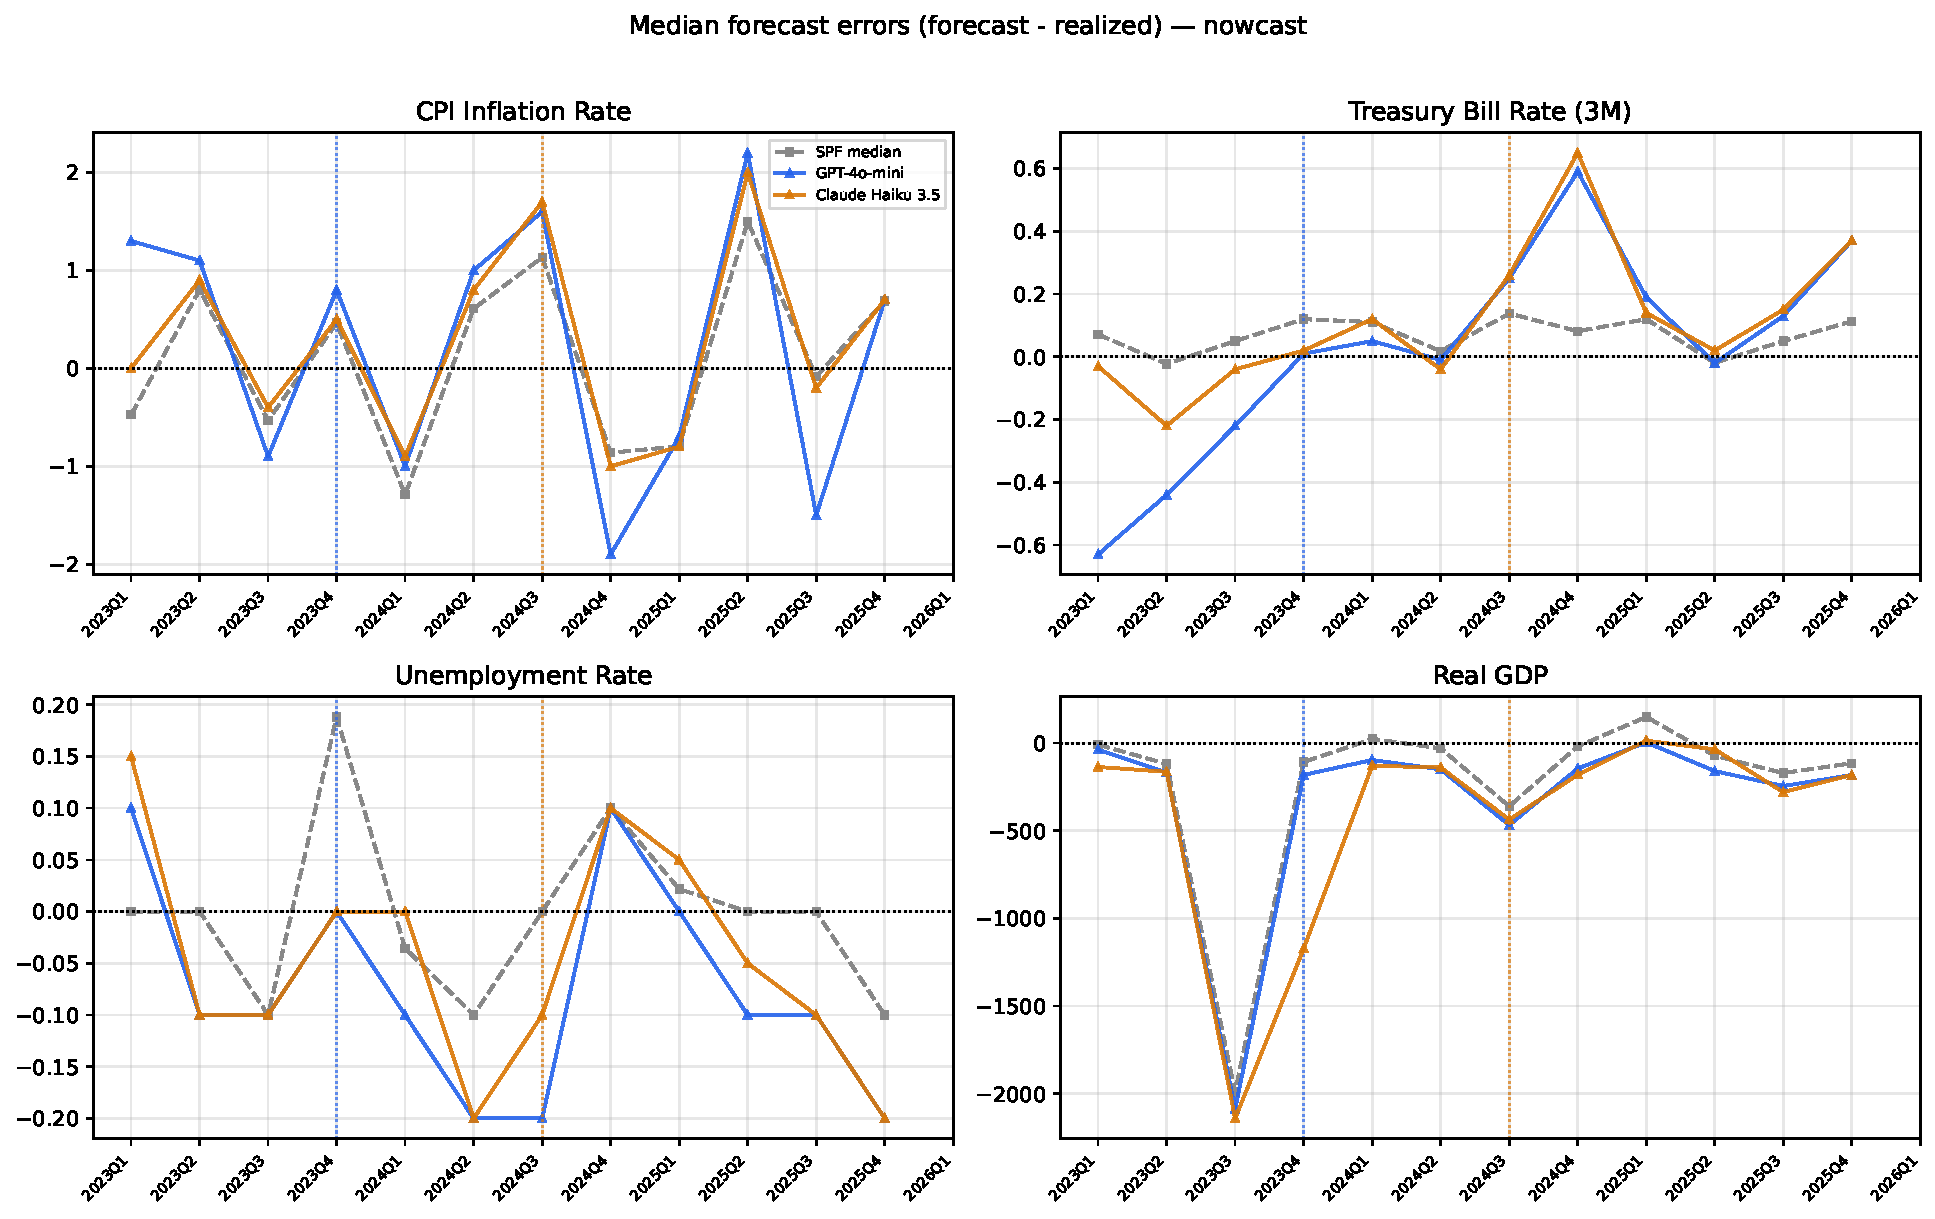
\includegraphics[width=\textwidth]{figures/oosnew/forecast_errors_oos_t.pdf}
    \caption{\textbf{SPF and AI-generated median forecast errors: nowcast}
    \vspace{5pt}\\
    {\footnotesize The figure shows nowcast forecast errors, defined as forecast minus realized target-quarter value, for median SPF and AI-generated forecasts for the CPI inflation rate, real GDP index, 3-month Treasury bill rate, and unemployment rate. The horizontal dotted line indicates zero forecast error. The vertical dotted lines indicate model-specific out-of-sample starts.}
    \vspace{5pt}}
    \label{fig:oos_errors_t_two_models}
\end{figure}

\clearpage

\begin{figure}[htpb!]
    \centering
    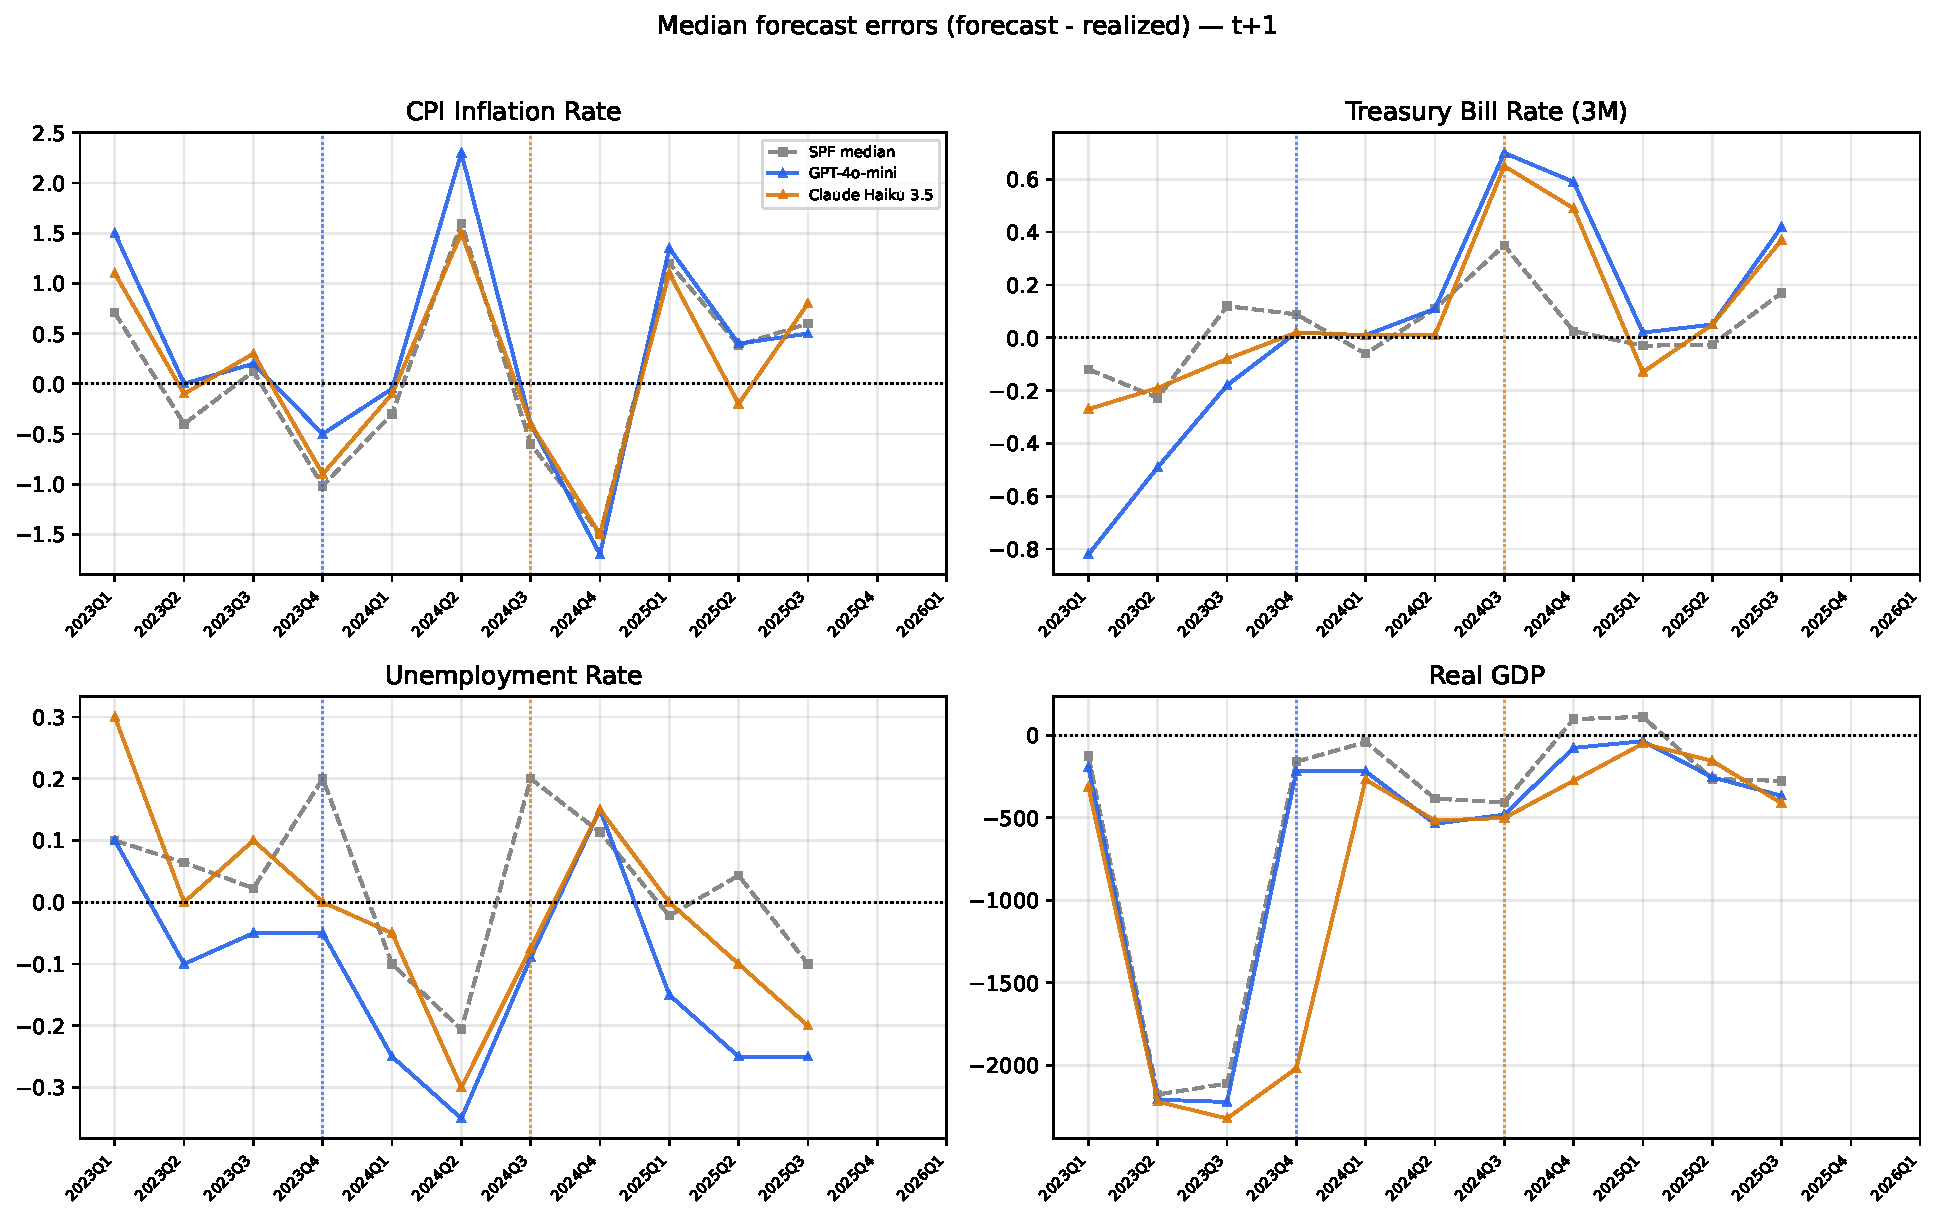
\includegraphics[width=\textwidth]{figures/oosnew/forecast_errors_oos_tp1.pdf}
    \caption{\textbf{SPF and AI-generated median forecast errors: one quarter ahead}
    \vspace{5pt}\\
    {\footnotesize The figure shows one-quarter-ahead forecast errors, defined as forecast minus realized target-quarter value, for median SPF and AI-generated forecasts for the CPI inflation rate, real GDP index, 3-month Treasury bill rate, and unemployment rate. The horizontal dotted line indicates zero forecast error. The vertical dotted lines indicate model-specific out-of-sample starts.}
    \vspace{5pt}}
    \label{fig:oos_errors_tp1_two_models}
\end{figure}
\end{comment}

\end{document}